\documentclass[a4paper,14pt]{extreport}


\usepackage{fontspec}
\setmainfont{Times New Roman}


\usepackage{setspace}
\onehalfspacing

\usepackage[backend = biber, bibencoding=utf8, sorting=nyvt, bibstyle=gost-numeric]{biblatex}

\usepackage[left=25mm, right=10mm, top=20mm, bottom=20mm]{geometry}

\addbibresource{bibliography.bib}

\usepackage{graphicx}
\usepackage[svgnames]{xcolor}

\usepackage{adjustbox}
\usepackage{caption}
\usepackage{amsmath}


\usepackage{cmap}					% поиск в PDF
\usepackage[T2A]{fontenc}
\usepackage[utf8]{inputenc}
\usepackage[english,russian]{babel}

\usepackage{csquotes}

\usepackage{color} 
\usepackage{hyperref}

\usepackage{listings}
\usepackage{protobuf/lang}
\usepackage{protobuf/style}

\lstset{
    backgroundcolor=\color{Gainsboro!60!Lavender},
    frame=tb, % draw a frame at the top and bottom of the code block
    tabsize=4, % tab space width
    showstringspaces=false, % don't mark spaces in strings
    numbers=left, % display line numbers on the left
    commentstyle=\color{green}, % comment color
    keywordstyle=\color{blue}, % keyword color
    stringstyle=\color{red} % string color
}

\usepackage[colorinlistoftodos]{todonotes}


\title{Разработка распределенной системы сбора данных и анализа формы импульса событий на установке \textquote{Троицк ню-масс}}
\author{Чернов Василий, ИЯИ РАН}
\date{\today}


\begin{document}

\thispagestyle{empty}
\begin{center}
\hfill \break
\normalsize{ФЕДЕРАЛЬНОЕ  ГОСУДАРСТВЕННОЕ БЮДЖЕТНОЕ УЧРЕЖДЕНИЕ НАУКИ}\\
\normalsize{ИНСТИТУТ ЯДЕРНЫХ ИССЛЕДОВАНИЙ РОССИЙСКОЙ АКАДЕМИИ НАУК} \\
\hfill \break
\hfill \break
\hfill \break
\normalsize{Чернов Василий Геннадьевич}\\
\hfill \break
\hfill \break
\normalsize{
    \textbf{Разработка распределенной системы сбора данных и \\анализа формы импульса событий на установке \\ \textquote{Троицк ню-масс}} \\
    }
\hfill \break
\normalsize{выпускная квалификационная работа} \\
\hfill \break
\hfill \break
Направление подготовки \\
\underline{03.06.01 Физика и астрономия} \\
\hfill \break
\hfill \break
Профиль подготовки \\
\underline{01.04.01 Приборы и методы экспериментальной физики} \\
\hfill \break
\hfill \break
Научный руководитель\\
\underline{Нозик Александр Аркадьевич, к. ф.-м. н.} \\
\hfill \break
\hfill \break
\hfill \break
\hfill \break
\hfill \break
\normalsize{ Москва-2019 }\\
\end{center}

\newpage

\setcounter{tocdepth}{3}
\tableofcontents
\newpage
\listoftodos
\todo[inline]{Часть глав в оглавлении без номера}

\chapter*{Введение}
\addcontentsline{toc}{chapter}{Введение}  

Одним из основных направлений в физике элементарных частиц является изучение свойств нейтрино. На данный момент экспериментально открыты три аромата частицы: электронные, мюонные и тау-нейтрино. Также экспериментально доказано наличие ненулевой массы нейтрино\todo{ссылка!}. Подобная конфигурация\todo{Конфигурация - странное слово, развернуть смысл} не может быть объяснена в рамках стандартной модели. Из-за этого изучение свойств (в нашем случае матрицу масс) нейтрино открывает возможность прямого исследования явлений новой физики.

На данный момент, полученные в ходе экспериментов ограничения на параметры нейтрино позволяют предположить существование еще одного нового вида частиц - стерильных (обладающих правой хиральностью). Теория не накладывает каких-либо непреодолимых ограничений на параметры массы и углов смешивания гипотетических стерильных нейтрино с <<активными>> нейтрино. Ограничения ставятся в основном экспериментально. Есть несколько аргументов в пользу существования таких частиц. Во-первых, т.к. для всех других видов фермионов были обнаружены как левосторонний, так и правосторонний варианты, существование нейтрино с обоими хиральностями выглядит адекватно. Также, существование стерильного нейтрино с определенными параметрами могло бы естественным образом объяснить наличие массы у активных нейтрино\todo{ссылка!}.

Эксперимент <<Троицк ню-масс>> некоторое время назад присоединился к поискам стерильного нейтрино \cite{1703.10779}. Не смотря на то, что установка была спроектирована для проведения прямых измерений массы активного электронного нейтрино, ее конструкция оказалась подходящей и для поиска стерильных нейтрино с массой в диапазоне до нескольких кэВ. Эта область значений масс недоступна в осцилляционных экспериментах, планирующихся в ряде мировых научных центров\todo{ссылки!}. 

Одной из целей данной работы является разработка программного комплекса для сбора данных на этой установке и первичному анализу этих данных. Этапы по достижению этой цели включают в себя разработку и реализацию новой архитектуры, с учетом современных методов разработки и подходов к построению систем. В основе новой системы был положен принцип максимальной модуляризации системы на отдельные, логически независимые и самостоятельные компоненты и создание высокоуровневого интерфейса взаимодействия между ними. Такой принцип значительно упрощает понимание и облегчает отладку и модернизацию системы. Третья глава содержит описание ахритектурного обновления системы сбора данных.

В четвертой главе представлены два примера расширения системы сбора данных с помощью встраивания и замены отдельных компонент. В первом примере описан случай прозрачной интеграции дополнительного модуля обработки сигнала, ведущего параллельный набор. Во втором примере описывается полная замена модуля системы сбора данных. Оба случая показывают преимущества модульности и наличия высокоуровнего командного интерфейса - упрощенная разработка, за счет небольшого функционала каждого из модулей и возможность простой замены или возврата к предыдущей конфигурации системы.

Основной целью данной работы является увеличение скорости набора данных до необходимого для поисков стерильного нейтрино уровня. Для этого было решено уменьшить мертвое время системы регистрации событий, перейдя на программную обработку непрерывного сигнала. В пятой главе представлены разработанные алгоритмы выделения параметров событий из непрерывного сигнала и разделения наложений.

\chapter{Эксперименты по поиску стерильных нейтрино}

Как уже упоминалось, параметры гипотетического стерильного нейтрино слабо ограничены с точки зрения теории, но максимальный интерес представляют три области масс:
\begin{itemize}
    \item Легкое стерильного нейтрино (масса порядка одного эВ). Такие легкие нейтрино могут объяснить ряд аномалий, наблюдаемых в экспериментальных данных. К примеру, результаты эксперимента LSND\cite{ссылка!}. В настоящее врямя, поиск таких нейтрино ведется в основном в осцилляционных экспериментах с короткой базой. Более подробный обзор экспериментов и соотвествующей теории представлен в \cite{light-sterile-neutrino-whitepaper}.
    
    \item <<Средние>> нейтрино с массами порядка нескольких кэВ представляют существенный интерес с точки зрения космологии, поскольку могут объяснить загадку темной материи. Именно в этом диапазоне ведет поиск эксперимент "Троицк ню-масс" и о нем пойдет речь в этой работе. \todo{ссылка на whitepaper по кэвным нейтрино}
    
    \item Тяжелые нейтрино с масcами свыше десятков МэВ интересны, поскольку могут позволить решить проблему генерации масс нейтрино в стандартной модели при помощи see-saw механизма и аналогичных теорий \todo{ссылку на see-saw, спросить у Ткачева}.
\end{itemize}

\section{Исследование спектра бета-распада трития}

Исторически, наиболее точным прямым методом поиска массы электронного нейтрино является исследование бета-спектра трития. Этот же процесс можно использовать и для поиска стерильных нейтрино средних масс. Небольшая примесь стерильного нейтрино с собственной массой, отличной от собственных масс активных компонент, при достаточном разрешении, проявится на форме спектра: на определенной энергии, соответствующей массе стерильного нейтрино, энергии кинематического процесса становится достаточно для испускания тяжелого стерильного нейтрино вместе с электронным \cite{new-tests-for-and-bounds-on-neutrino-masses-and-lepton-mixing}\cite{role-of-sterile-neutrino-warm-dark-matter-in-rhenium-and-tritium-beta-decays}\cite{signatures-of-extra-dimensional-sterile-neutrinos}\cite{sterile-neutrinos-and-right-handed-currents-in-katrin}.

Измеряемый спектр является взвешенной суперпозицией соответствующих собственной массе для каждого аромата нейтрино спектров с весом, равным амплитуде перехода из текущего аромата нейтрино в электронный (элемент $ U_{e i} $ в матрице смешиваний; здесь i - текущий аромат). Т.к. различие масс между электронным, мюонным и тау-нейтрино слишком мало, чтобы быть различимым в каком либо из действующих экспериментов, вместо суперпозиции состояний используется спектр, соответствующий одной эффективной легкой массе нейтрино, соответствующей формуле \ref{effective-light-neutrino-mass}.

\begin{equation}\label{effective-light-neutrino-mass}
   m(\nu_{e})^2 = \sum_{i=1}^{3} \mid U_{e i} \mid^2m(\nu_{i})^2  
\end{equation}

В случае, если электронный нейтрино имеет примесь собственной массы $ m_s $ порядка $O(1)$ кэВ, суммарный спектр будет состоять суммы спектра эффективной легкой массы нейтрино и спектра $ m_s $ и иметь дифференциальную форму, описывающуюся формулой \ref{beta-decay-summary-spectrum}.
\begin{equation}\label{beta-decay-summary-spectrum}
    \frac{d}{d\Gamma} = cos^2(\theta) \frac{d}{d\Gamma} (m(\nu_e)) + sin^2(\theta) \frac{d}{d\Gamma} (m_s)
\end{equation}
На графиках \ref{fig:beta-decay-kink} показаны качественные примеры идеальных формы спектра, на которых легко заметить сигнатуры стерильных нейтрино.
\todo[inline]{Мне эти картинки сильно не нравятся. Я в свое время на них сильно ругался. Не говоря уже о том, что надо писать, откуда берешь. Я думаю, что надо заменить. У меня где-то лежат}
\begin{figure}
  \centering
  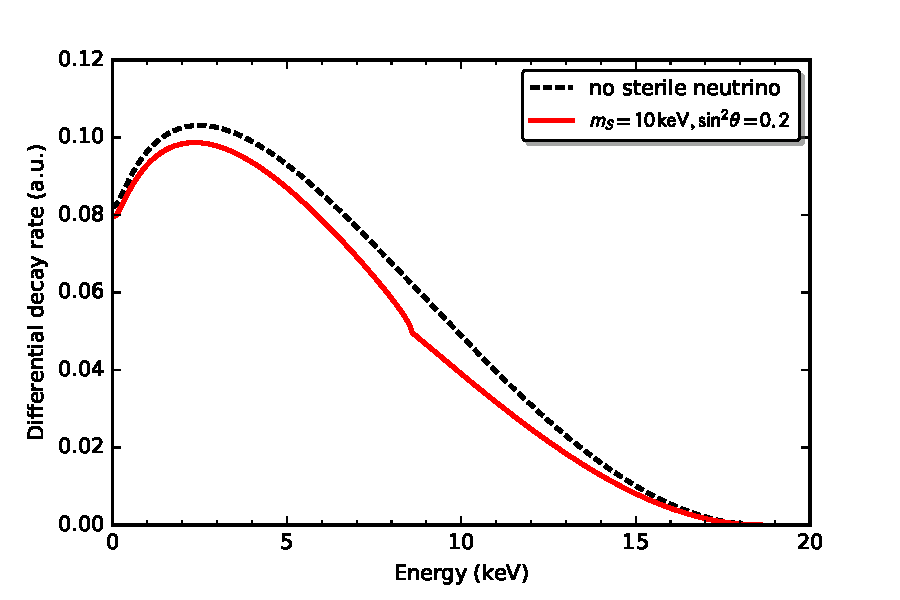
\includegraphics[width = 0.49\textwidth]{img/beta_decay/PlotKink.pdf}
  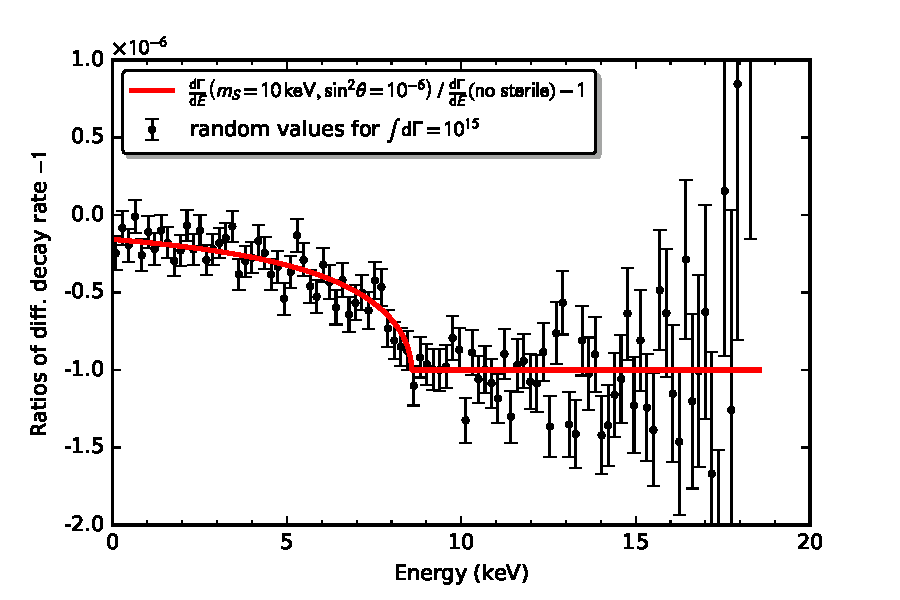
\includegraphics[width = 0.49\textwidth]{img/beta_decay/PlotRatio.pdf}
  \caption{a: Сравнение спектров $\beta$-распада трития без смешивания (черная пунктирная линия) со смешанным со стерильным нейтрино массой 10 кэВ и углом смешивания $\sin^{2}\theta=0.2$ (красная линия). На графике легко заметить сигнатуру в виде перегиба в точке $E = E_0 - m_{\mathrm{s}}$ искажение формы перед перегибом. b: Сравнение спектров $\beta$-распада трития без смешивания (черная пунктирная линия) со смешанным со стерильным нейтрино массой 10 кэВ и углом смешивания  $\sin^{2}\theta=10^{-7}$. Ошибки советуют симуляции $\sim 10^{18}$ электронов.}
 \label{fig:beta-decay-kink}
\end{figure}

Исследование бета распада трития для поиска стерильных нейтрино с массой порядка кэВ имеет очевидные преимущества: процесс распада имеет сверх-разрешенный тип, поэтому форма спектра описывается точной теоретической формулой. Также тритий имеет относительно небольшое время полураспада и может, при небольшом объеме источника, обеспечить высокую скорость счета (небольшой объем также минимизирует систематические эффекты, связанные с источником). Наконец, тритий имеет граничную энергию бета спектра $ E_0 = 18.575 $ кэВ, благодаря которой можно проводить поиски в интересном для астрофизиков диапазоне масс.

Анализ спектра бета-распада трития используется в экспериментах:
\begin{itemize}
	\item <<Троицк ню-масс>> - в качестве источника используется тритиевый газ; набор спектра осуществляется в интегральном режиме с помощью большого цилиндрического спектрометра, который останавливает частицы по порогу энергии;  установка будет подробно описана в работе.
	\item <<Katrin>>\cite{katrin-design-report-2004}\cite{current-direct-neutrino-mass-experiments} - установка по принципу работы и структуре схожа с <<Троицк ню-масс>>, однако имеет значительно больший масштаб. Увеличенные размеры позволяют достигнуть разрешающей способности в 200 мэВ.
	\item <<Project 8>>\cite{rel-cyclotron-tritium}\cite{single-electron-detection-and-spectroscopy-via-relativistic-cyclotron-radiation}, <<Ptolemny>>\cite{ptolemy} - эксперименты исследуют излучение бета электронов в циклотроне, используется источник атомного трития.
\end{itemize}

\section{Электронный захват}

Еще одним перспективным способом для поиска является исследование калориметрически измеренного спектра электронного захвата  $ ^{163}Ho $ . Выбор вещества обусловлен его низкой энергией, доступной для распада равной $Q_{E C} = 2.833 \pm 0.030_{stat} \pm 0.015_{syst} $ кэВ\cite{1604.04210}\cite{0911.3329}, благодаря которой на границах энергетического спектра сохраняется достаточная скорость счета и хорошая статистика. Как следствие, в задаче определении массы нейтрино, подход может добиться такой же точности, что и большой эксперимент Katrin.

На данный момент есть три больших коллаборации, использующие калориметрический спектр электронного захвата  $ ^{163}Ho $ и ориентированные на набор статистики большого размера и высокой точности: <<Electron Capture in  $ ^{163}Ho $ (ECHo)>>\cite{1309.5214}, <<Electron Capture Decay of  $ ^{163}Ho $ to Measure the Electron Neutrino Mass with sub-eV sensitivity (HOLMES)>>\cite{1412.5060}, <<Neutrino Mass via  $ ^{163}Ho $ Electron Capture Spectroscopy (NuMECS)>>\cite{numex-position-paper}. Сейчас коллаборации нацелены на измерения массы нейтрино, однако, т.к. при калориметрических измерениях каждое событие создает измеримый сигнал и может быть записано, установки способны набрать спектр во всем диапазоне и провести поиск стерильного нейтрино.

Сигнатура стерильных нейтрино, как и в тритиевом бета спектре, проявляется на спектре в виде небольшого перегиба. Подробнее про модель спектра можно прочитать в \cite{dm-kev-sterile-neutrino-whitepaper}. По спектру $ ^{163}Ho $ можно определить существование стерильных нейтрино в диапазоне до $ Q_{E C} = 2.5 $ кэВ. На графиках \ref{fig:ste-kink} показано сравнение модельных форм спектров.

\begin{figure}
  \centering
  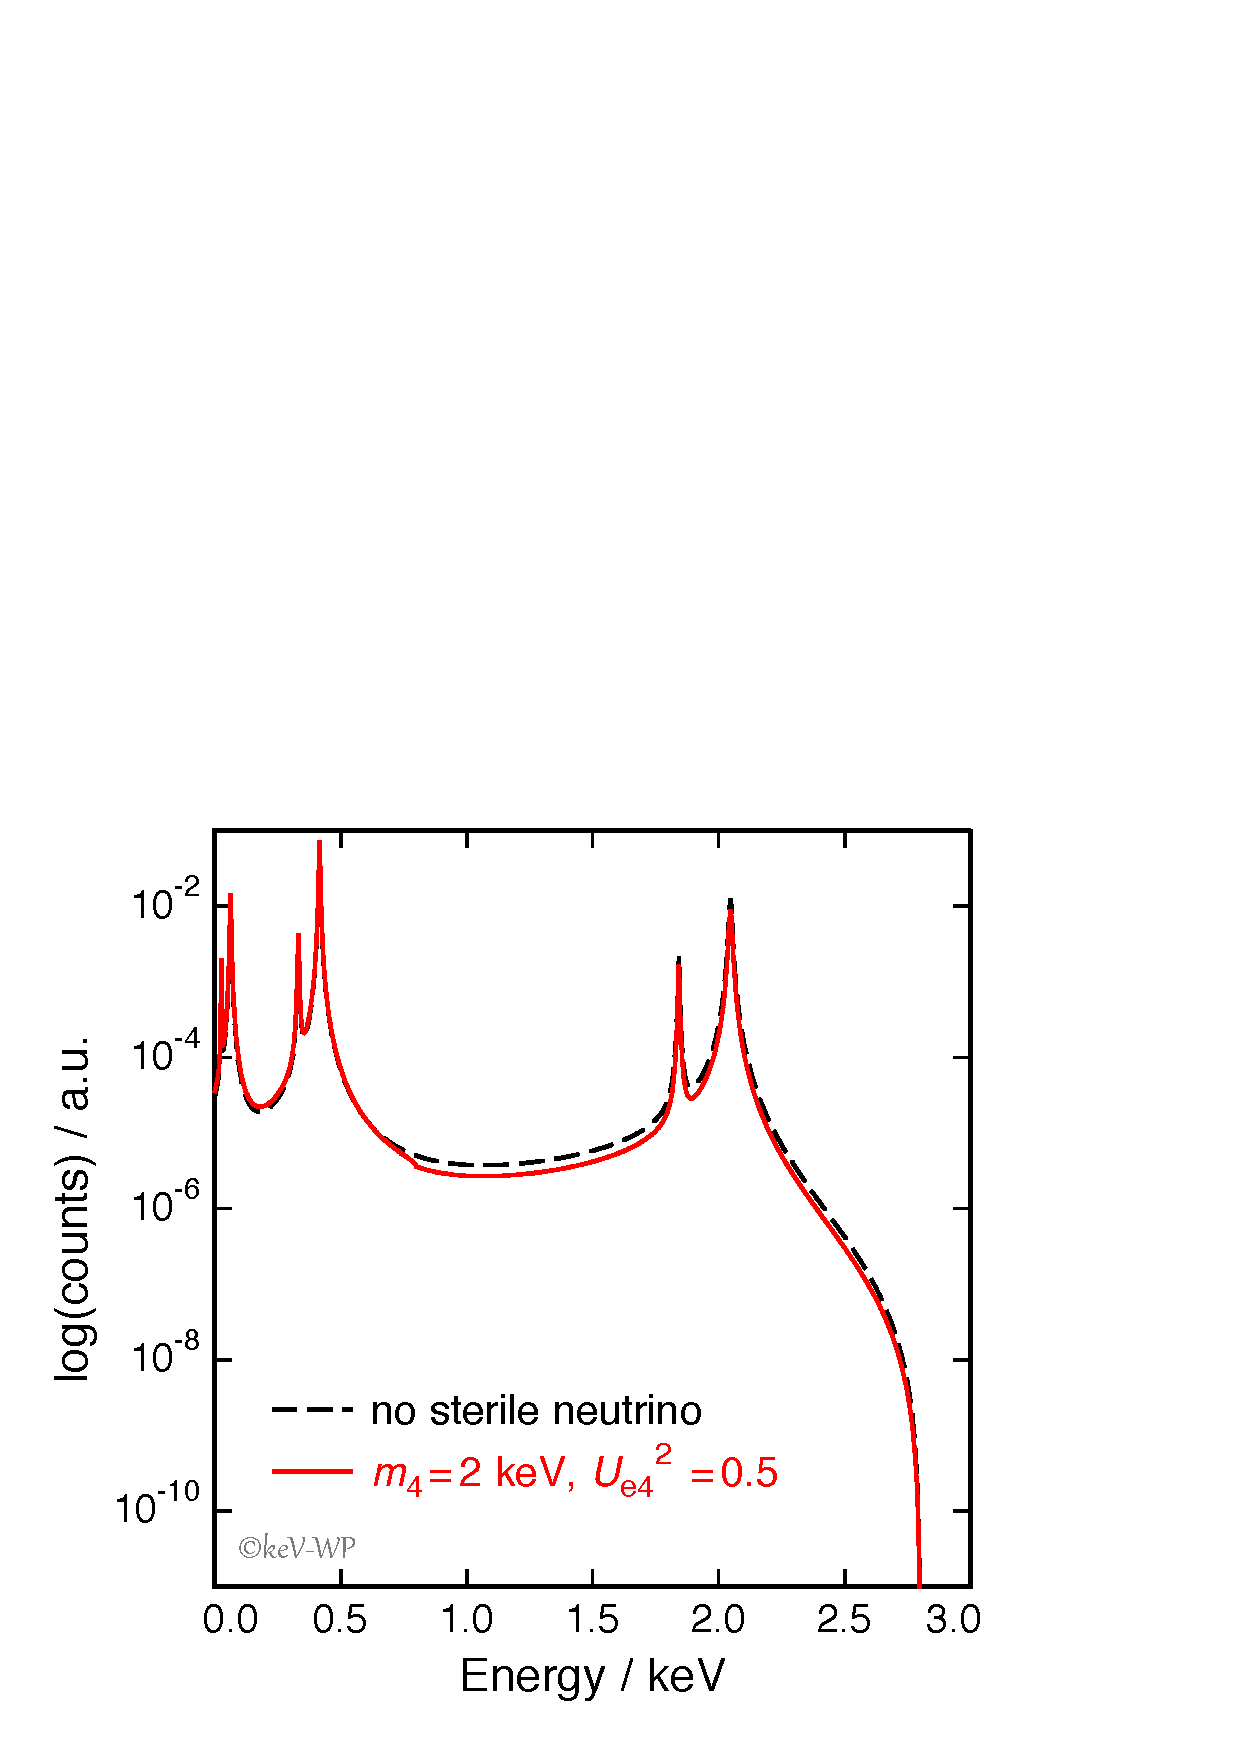
\includegraphics[width = 0.45\textwidth]{img/electron_capture/ste_full_spe.pdf}
  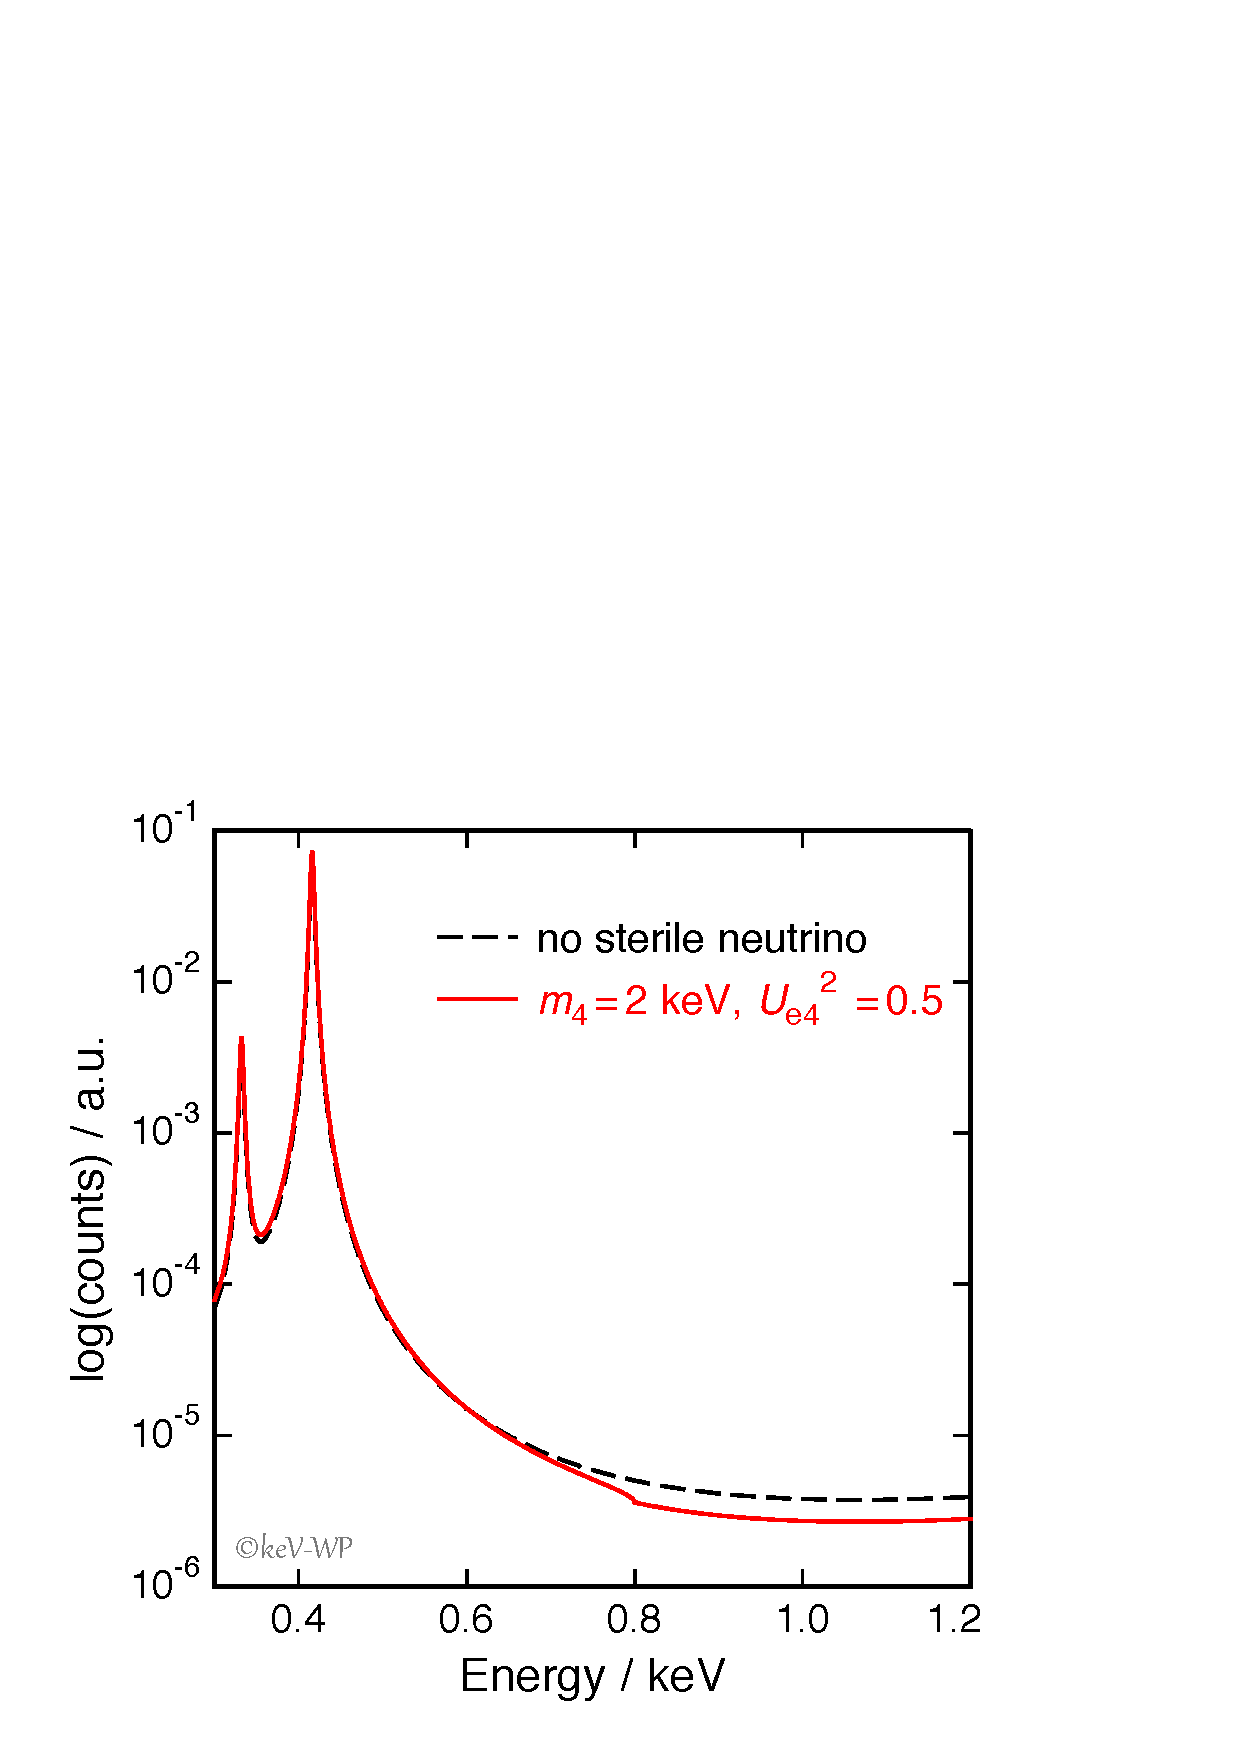
\includegraphics[width = 0.44\textwidth]{img/electron_capture/ste_det_spe.pdf}
    \caption{a) Сравнение калориметрических спектров $ ^{163}Ho $ без воздействия стерильных нейтрино (черная пунктирная линия) и с воздействием тяжелых стерильных нейтрино с массой $m_4=2$ кэВ и коэффициентом смешивания $U_{\mathrm{e4}}^2 = 0.5$. b) Приближение (a) в область перегиба.}
    \label{fig:ste-kink}
\end{figure}

\section{Прямое измерение нейтрино}

В данном способе измеряются свойства реликтовых стерильных нейтрино. Подход имеет свои особенности. Из положительных можно отметить, что такие измерения помимо поиска стерильных нейтрино также исследуют природу и свойства темной материи. Т.о. эксперимент, в случае соответствия модели, станет убедительным доказательством того, что темная материя состоит из стерильных нейтрино, а, в случае несоответствия - данные все равно могут быть использованы для проверки других гипотез о темной материи.

Прямые измерения могут быть реализованы через захват космических электронных нейтрино радиоактивными ядрами, испытывающими бета-распад\cite{1005.3351}\cite{1009.5870}. Посредством смешивания с активным электронным (анти) нейтрино $\nu_e (\bar{\nu}_{e})$, кандидат на темную материю $ {N}^{}_{1} $ массой порядка $O(1)$ может подвергаться реакции захвата $ {N}^{}_{1} + \mathcal{N}(A,Z) \to \mathcal{N}^\prime (A, Z\mp1) + e^{\pm} $, где A, Z - массовый и атомный номера исходного ядра соответственно. Сигнатуры реакций захвата измеряются через испускаемые в результате моноэнергетические электроны (позитроны), энергия которых находится за границей энергий соответствующего бета распада. Измерение расстояния между процессами распада и захвата напрямую определит наличие стерильных нейтрино с массой порядка кэВ в темной материи и определит соответствующие массу и коэффициенты смешивания.

\chapter{Установка <<Троицк ню-масс>>}

\begin{figure}
  \centering
  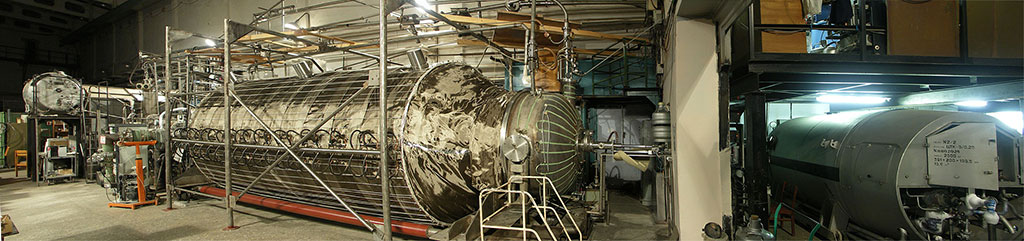
\includegraphics[width = 0.99\textwidth]{img/nu_mass_setup/setup.jpg}
    \caption{Установка <<Троицк ню-масс>>.}
    \label{fig:numass-photo}
\end{figure}

Установка предназначена для проведения прецизионных измерений бета спектров от трития в диапазоне энергий от 5 кэВ до порядка 35 кэВ. В основе ее работы лежит 
принцип так называемого адиабатического движения электронов в магнитном поле. Под адиабатичностью движения здесь подразумевается не отсутствие потерь энергии (магнитное поле не совершает работы над заряженной частицей, поэтому потерь быть и не может), а движение электрона вдоль одной силовой линии.

\todo[inline]{Рисунок старый, надо взять с новым спектрометром
}
На рисунке \ref{fig:numass-general} схематично изображены компоненты <<Троицк ню-масс>>. Установка состоит из: интегрального электростатического спектрометра с магнитной адиабатической коллимацией, безоконного источника электронов с молекулярным тритием в газообразном состоянии, вакуумной системы откачки, криогенной системы, обеспечивающей рабочую температуру сверхпроводящих соленоидов спектрометра и термостабилизацию источника, высоковольтную систему и систему сбора данных.

\begin{figure}
  \centering
  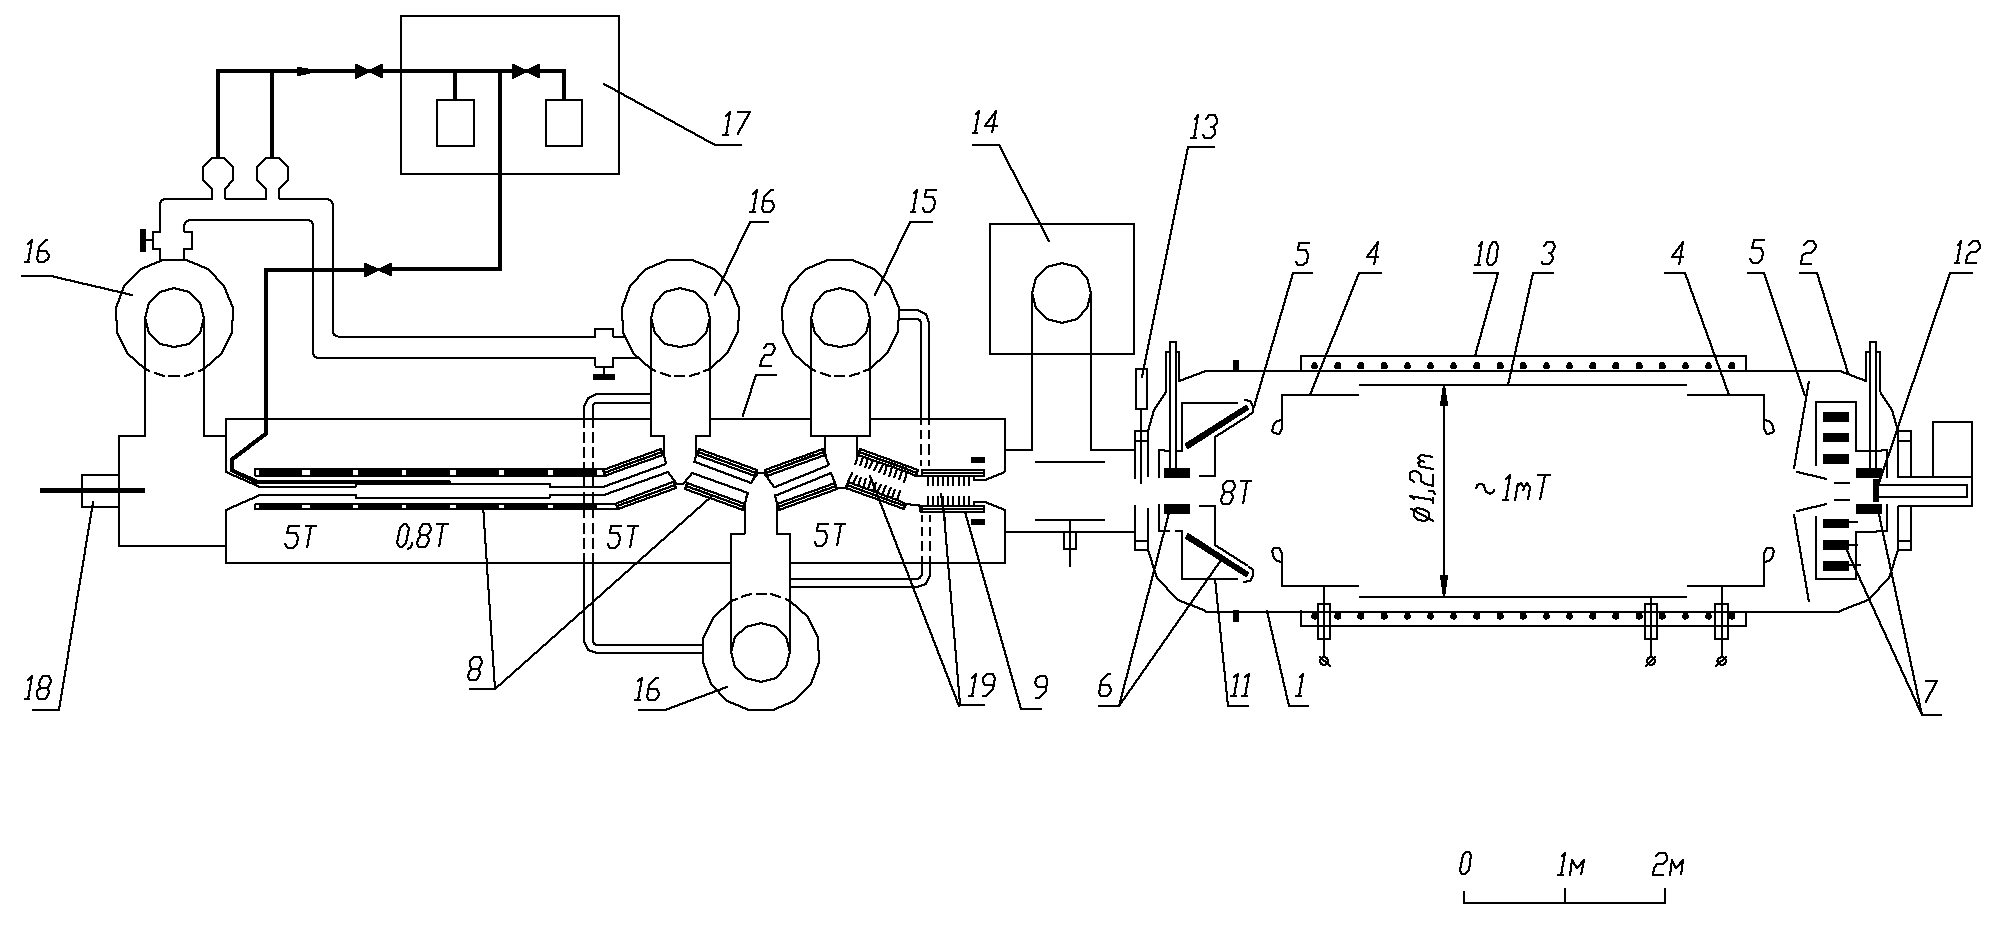
\includegraphics[width = 0.99\textwidth]{img/nu_mass_setup/general.png}
    \caption{Схема установки. Обозначения: 1, 2 – вакуумный объем; 3, 4 – электростатическая система; 5 – заземленный электрод; 6–9 – сверхпроводящие магниты; 10 – теплый соленоид; 11 – азотный экран; 12 – Si(Li) детектор; 13 – аварийный шибер; 14 – магниторазрядный насос; 15, 16 – ртутные диффузионные насосы; 17 – система очистки трития; 18 – электронная пушка; 19 – аргоновая ловушка.}
    \label{fig:numass-general}
\end{figure}

Безоконный тритиевый источник представляет собой трубу длиной 3 м и диаметром 5 см, помещенную внутрь криостата со сверхпроводящими магнитами, который генерирует внутри источника аксиальное поле с величиной потенциала до 0.8 Тл.

Торец источника со стороны спектрометра соединен с системой магнитной транспортировки, которая перемещает электроны бета-распада газообразного трития в объем спектрометра. Поле внутри системы достигает значений 5 Тл и ее коллимационные магниты расположены под углом друг к другу образуя путь в виде <<зигзага>>, не имеющий сквозного прямого пути. Такая конфигурация магнитов препятствует прохождению незаряженных частиц в спектрометр.

На рисунке \ref{fig:numass-spectrometer} изображен электростатический спектрометр, используемый на установке.

\begin{figure}
  \centering
  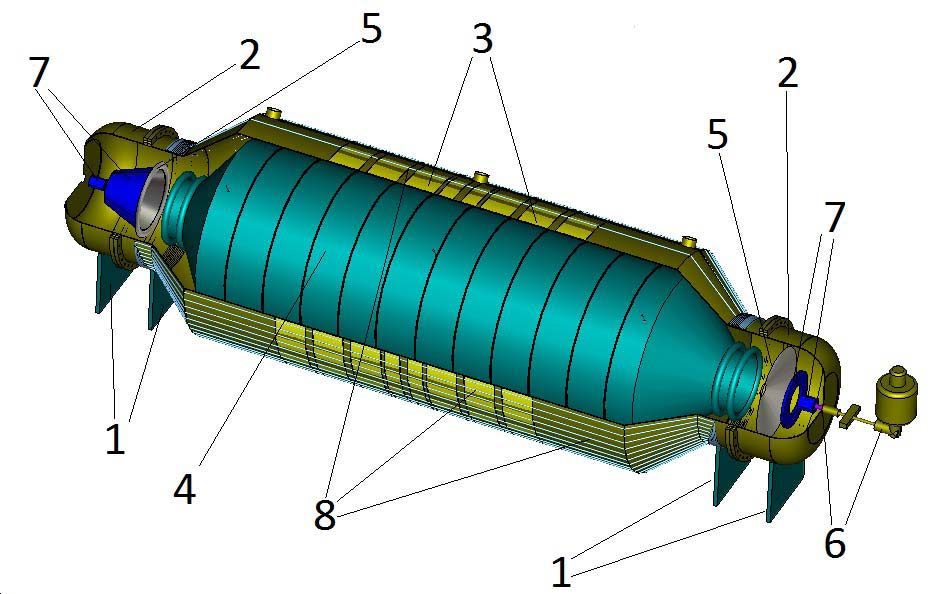
\includegraphics[width = 0.99\textwidth]{img/nu_mass_setup/spectrometer.jpg}
    \caption{Схема спектрометра. Обозначения: 1 - опоры спектрометра, 2 - входная и выходная чашки, 3 - теплые аксиальные обмотки, 4 - основной высоковольтный электрод, 5 - электроды под нулевым потенциалом, 6 - система детектора с охлаждением жидким азотом, 7 - набор сверхпроводящих магнитов.}
    \label{fig:numass-spectrometer}
\end{figure}

Спектрометр работает в интегральном режиме. С помощью высоковольтной системы на основной высоковольтный электрод подается запирающее напряжение. При прохождении электрона, в случае, если его энергия превышает выставленное запирающее напряжение - электрон проходит потенциальный барьер и попадает в установленный за ним детектор. Электроны с более низкими энергиями отражаются от потенциала и не доходят до детектора. Проведя серию наборов событий при разных значениях запирающего напряжения мы получим и интегральный спектр энергий рожденных во время бета-распада трития электронов. Разрешающая способность спектрометра определяется его геометрией и может потенциально достигать долей электронвольта\todo{до этого момента KATRIN не упомяналась. Надо сделать кусок описания в предыдущих главах и поставить туда ссылку} \cite{katrin-design-report-2004}. Использование спектрометра позволяет значительно снизить требования к разрешению детектора, т.к. оно перестает быть определяющим фактором. Амплитуды зарегистрированных событий используются в основном для контроля качества набора,  поиска и фильтрации аномальных событий, (в принципе можно использовать детектор и в счетном режиме). Адиабатичность переноса электронов в спектрометре обеспечивается конфигурацией магнитного поля спектрометра, которое формируется с помощью системы сверхпроводящих соленоидов, размещенных на поверхности.

Т.к. в работе будет рассматриваться в основном система управления набором - рассмотрим подробнее элементы системы, делая акцент на особенности управления и способы автоматизации контроля.

\section{Тритиевый молекулярный источник электронов}

На рисунке \ref{fig:numass-source} представлена схема тритиевого источника.

\begin{figure}
  \centering
  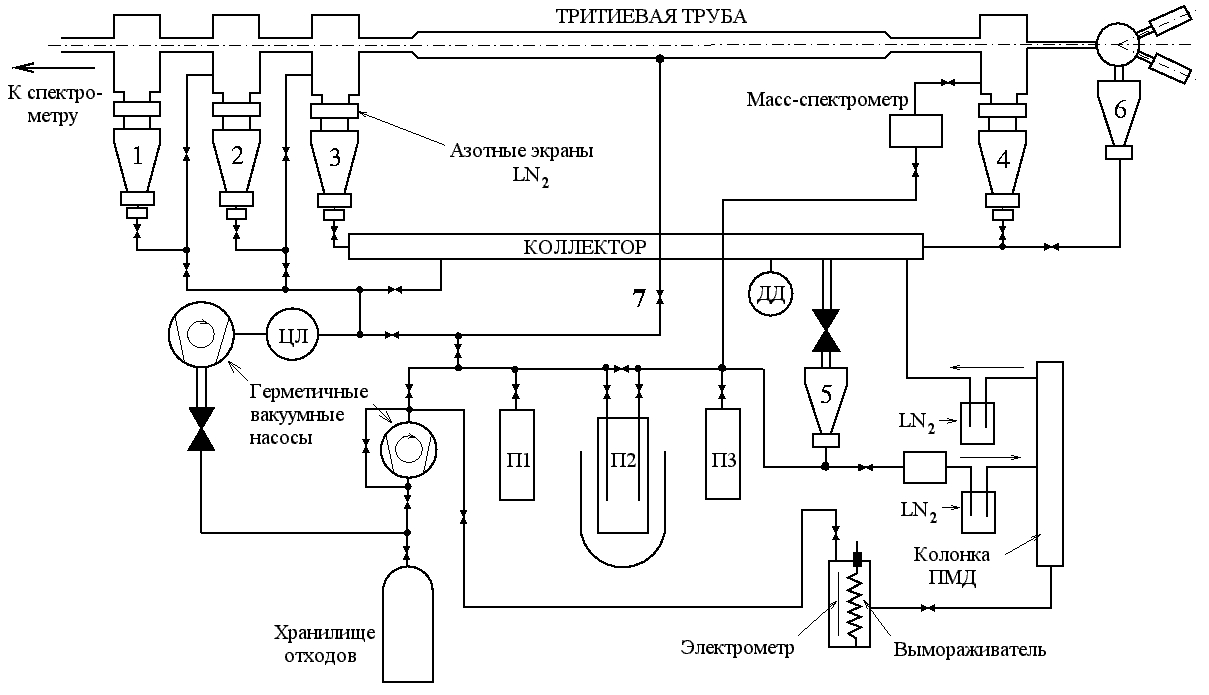
\includegraphics[width = 0.99\textwidth]{img/nu_mass_setup/source-control.png}
    \caption{Схема тритиевого источника. Обозначения: 1 – ртутный насос «P4»; 2 – ртутный насос «P3»; 3 – ртутный насос «P2»; 4 – ртутный насос «P1»; 5 – бустерный ртутный насос; 6 – ртутный насос откачки задней секции; 7 – натекатель; ЦЛ – цеолитовая ловушка; ДД – датчик давления; П1 – патрон-хранилище; П2 – очистной патрон; П3 – транспортный контейнер.}
    \label{fig:numass-source}
\end{figure}

\todo[inline]{Кажется, что я это уже где-то писал. Не забудь проверить, чтобы у тебя не было сильно много прямых текстуальных заимствований, поскольку дисеры могут проверять на антиплагиате}
Низкая граничная энергия бета-распада трития (18575 эВ) с одной стороны обеспечивает возможность установки достаточного напряжения на спектрометре. С другой стороны такие низкие энергии делают принципиально невозможным создание какого-либо барьера между объемами спектрометра и источника. Поэтому между источником и спектрометром должна находится мощная система перехвата и откачки газа, обеспечивающую снижение концентрации трития по пути от источника к спектрометру практически на 10 порядков - от $ 5 * 10^{14} \textbf{см}^{-3}$ в источнике до  $ 10^{5} \textbf{см}^{-3}$ в спектрометре.На практике выполнение таких требований реализуется системой из пяти ртутных насосов: 3 насоса (<<P1>>, <<P2>>, <<P3>>) расположены между тритиевой трубой источника и спектрометра, один - между тритиевой трубой и задней секцией (<<P4”) и один аргоновый насос прямо перед спектрометром. К откачному порту насоса <<P4>> подключен масс-спектрометр МХ-7340, используемый для анализа и мониторинга изотопного состава газа в источнике. Насосы <<P1>>, <<P2>>, <<P3>> объединены в цепь дифференциальной откачки (т.е. в последовательную цепь, где выхлоп насоса соединяется с откачным портом следующего насоса т.о. обеспечивая более высокий предельный вакуум). Откачанный насосами газ попадает в коллектор, где с помощью бустерных насосов прогоняется через систему изотопной очистки, а затем через тонкий натекатель возвращается обратно в тритиевую трубу. Таким образом, осуществляется замкнутый контур циркуляции трития в системе.

Помимо мощной системы откачки источник также требует термостабилизации трития: т.к. он находится при температурах порядка 30 К даже небольшие колебания температуры способны значительно изменить концентрацию газа и соответственно повлиять скорость счета набираемых данных (флуктуации в 1 К меняют концентрацию трития более чем на 3 \%).

Система источника управляется вручную. В процессе набора данных проводится автоматизированный мониторинг давлений в насосах, температуры и изотопного состава источника.

\section{Спектрометр}
Спектрометр представляет собой цилиндр диаметром 2.6 м и длиной 8 м, внутри которого на электроизолирующих подвесах установлен цилиндрический подключенный к высоковольтной стойке электростатический электрод, создающий основной запирающий потенциал. Внешний цилиндр с торцов закрывается полусферическими “чашками”, внутри которых располагаются сверхпроводящие магниты: пинч-магнит со стороны источника и магнит детектора. Эти магниты корректируют поле основного электрода делая из него магнитную “бутылку” в спектрометре (качественно форма изображена на рисунке \ref{fig:numass-spectrometer-fields}).

\begin{figure}
  \centering
  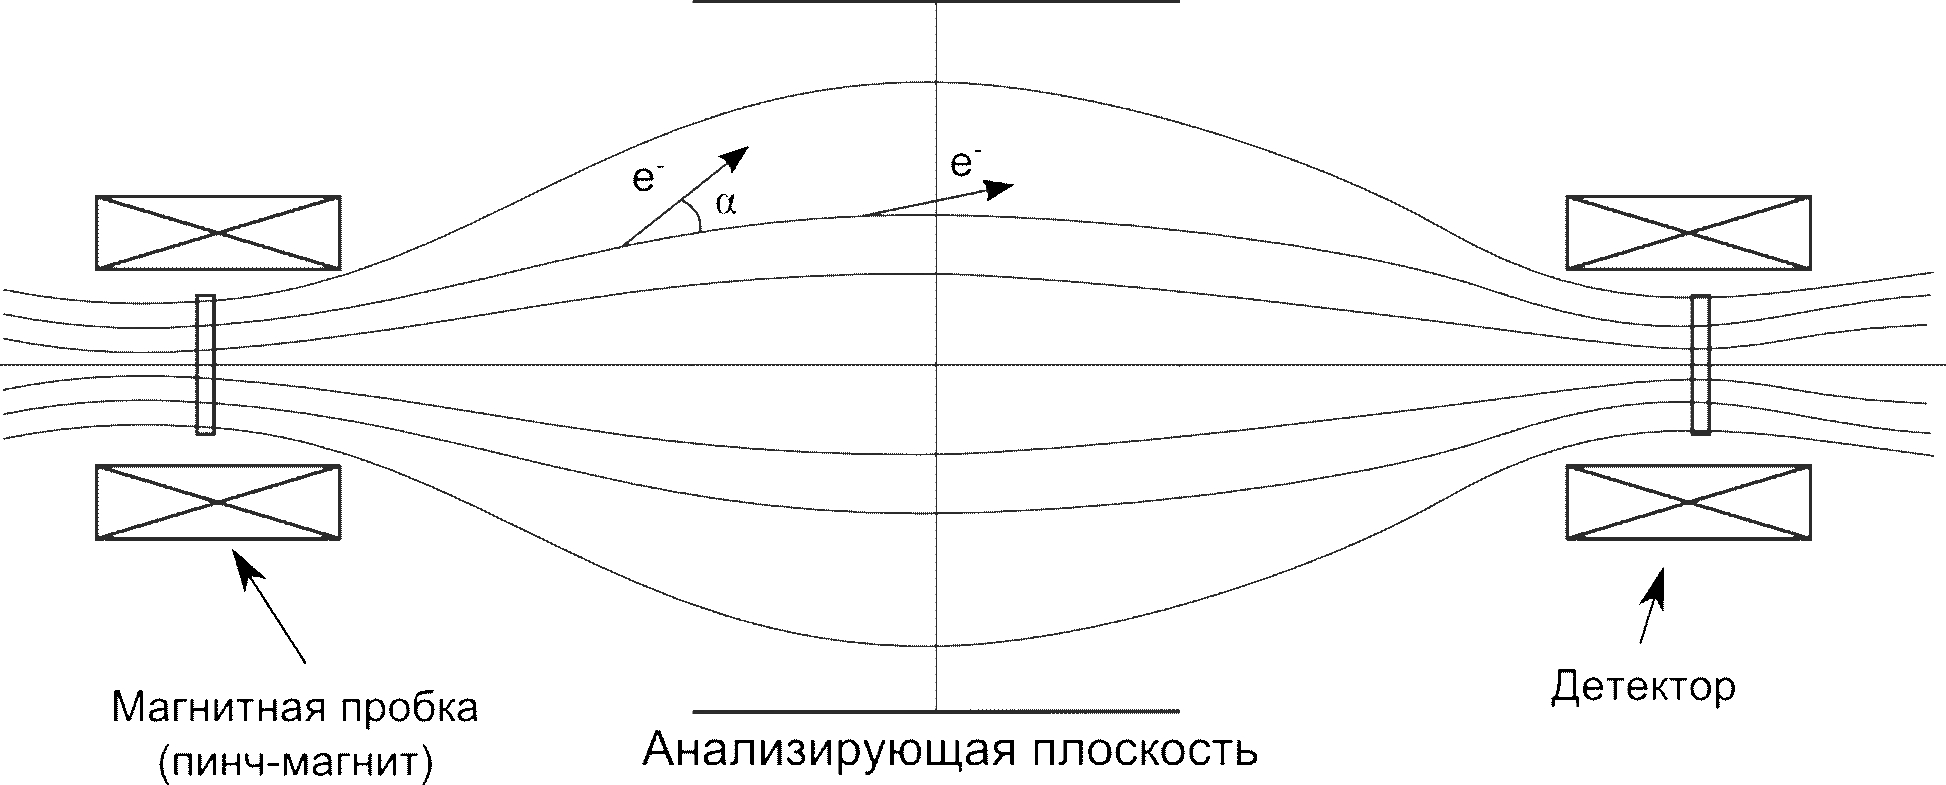
\includegraphics[width = 0.99\textwidth]{img/nu_mass_setup/spectrometer-fields.png}
    \caption{Конфигурация магнитного поля внутри спектрометра.}
    \label{fig:numass-spectrometer-fields}
\end{figure}

Для обеспечения плавности изменения диаметра трубки тока по мере прохождения спектрометра в чашках также находятся согласовывающие магниты. На поверхности спектрометра расположены еще три электромагнитные системы в виде продольных и аксиальной обмоток, образующих сетку. Они используются для дополнительной коррекции магнитного поля в центре спектрометра - две из них компенсируют магнитное поле земли и другие внешние поля,  третья аксиальная позволяет сужать трубку и держать силовые линии внутри объема электрода. 

Во время набора, спектрометр управляется автоматизировано через контроль\todo{управляется через контроль?} подающегося на электрод напряжения, выполняемый с помощью аппаратной части высоковольтной системы. Управление токами формирующих магнитов также автоматизированно.

\section{Криогенная система}

Криогенная система установки <<Троицк ню-масс>> осуществляет поддержание необходимой для обеспечения сверхпроводимости температуры на соленоидах спектрометра и термостабилизацию трубки источника. Схема криогенной системы показана на рисунке \ref{fig:numass-cryogenic}.

\begin{figure}
  \centering
  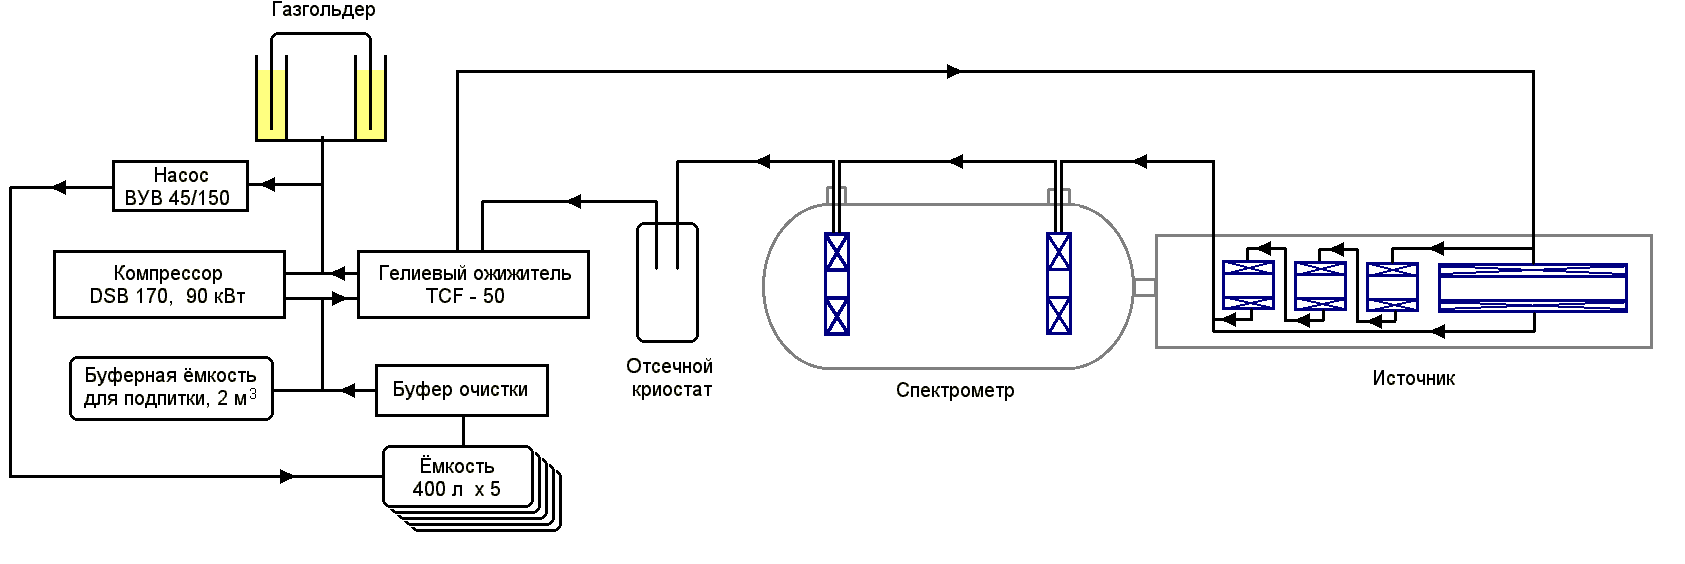
\includegraphics[width = 0.99\textwidth]{img/nu_mass_setup/cryogenic.png}
    \caption{Схема криогенной системы.}
    \label{fig:numass-cryogenic}
\end{figure}

Охлаждение криостатов осуществляется через циркуляцию по ним жидкого гелия, который проходит последовательно от криостатов трубки и соленоидов источника через криостаты спектрометра в ожижитель TCF-50. Для снижения теплопотерь и уменьшения нагрузки на рефрижератор, гелиопроводные трубы помещаются в экраны наполненные жидким азотом. Азотные экраны имеют свою, независимую от гелия, систему циркуляции. Помимо этого с помощью отдельных дьюаров на установке осуществляется охлаждение детектора, электронной пушки и откачивающих и бустерных насосов. Более подробная схема работы криогенной системы описана в \cite{cryogenic-1}\cite{cryogenic-2}.

\section{Электронная пушка}
Схема электронной пушки, использующейся на установке Троицк ню-масс изображена на рисунке \ref{fig:numass-gun}.

\begin{figure}
  \centering
  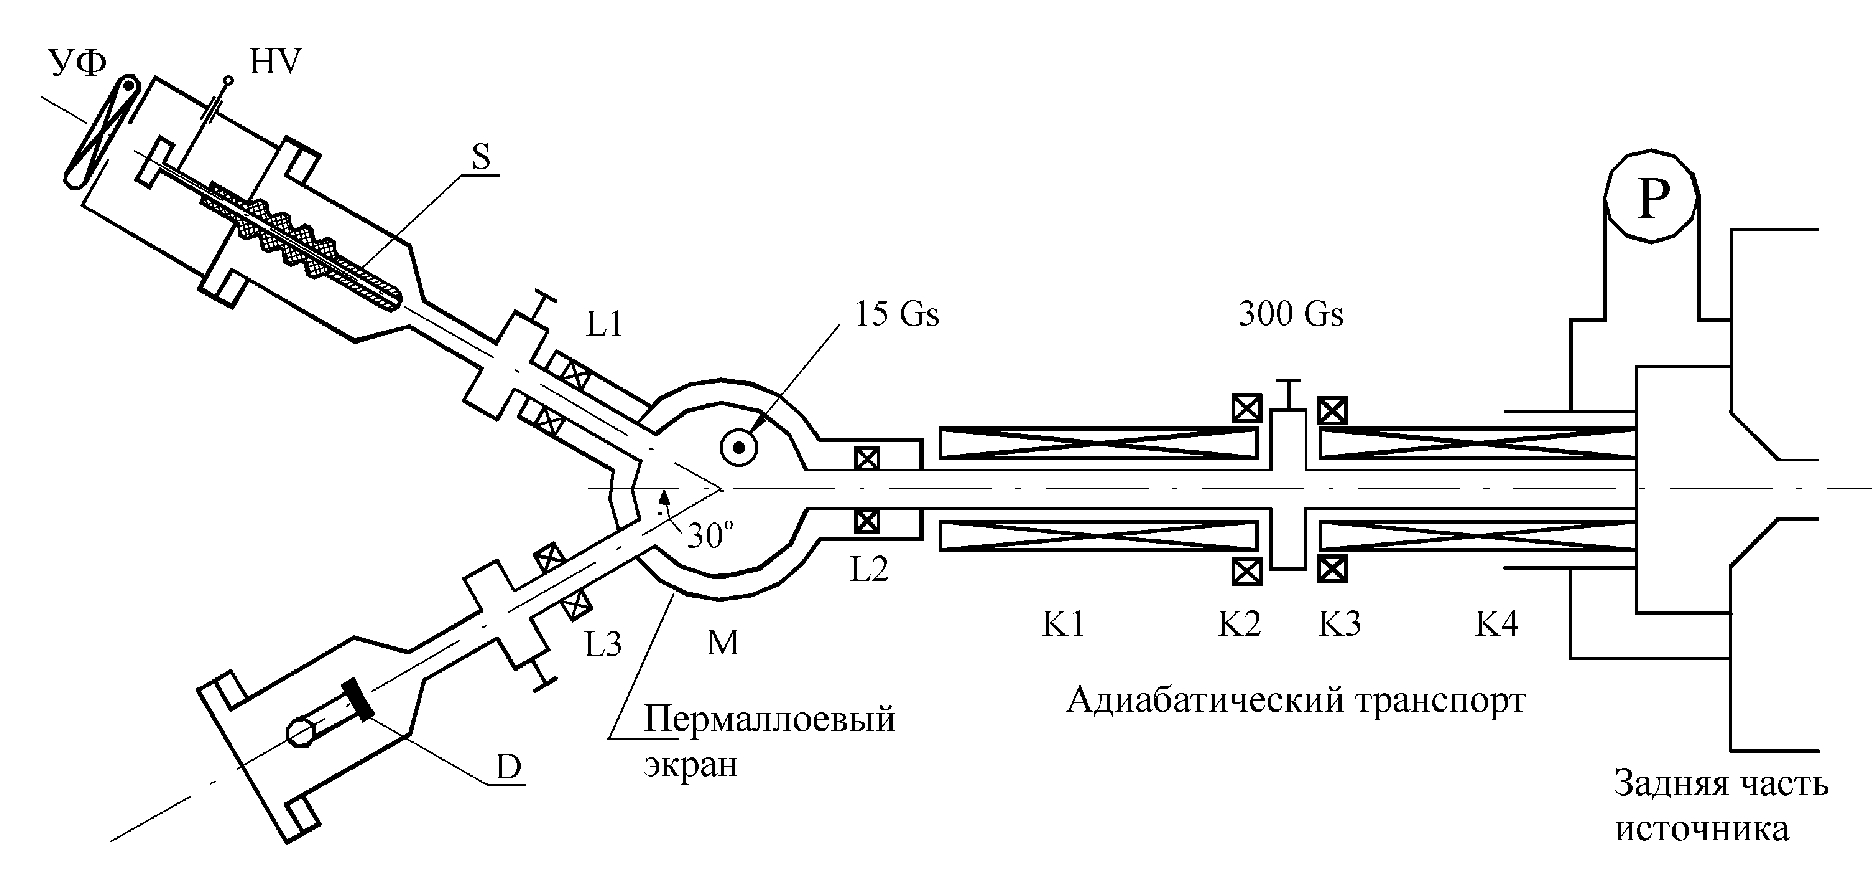
\includegraphics[width = 0.99\textwidth]{img/nu_mass_setup/gun.png}
    \caption{Схема электронной пушки.}
    \label{fig:numass-gun}
\end{figure}

Принцип работы основан на выбивании электронов с золотой поверхности с помощью ультрафиолета и последующего их ускорения в электростатическом поле до нужных энергий. В пушке предусмотрена фильтрация электронов от фотонов УФ лампы и ионов источника исполненная в виде поворотного магнита, расположенного после ускоряющего конденсатора. Ускоряемые в сторону поверхности с золотым напылением ионы при столкновении с ней производят дополнительные электроны тем самым увеличивая эффективность пушки.

После поворотного магнита по пути следования электронов расположены коллимационные магнитные линзы обеспечивающие сохранение углового распределения электронов. После настройки поворотного и коллимационных магнитов пушки выходное распределение электронов изотропно и имеет максимальный угол вылета = 0.0513 рад. Подробнее о строении и калибровке пушки написано в \cite{zadorogny}.

\section{Сбор данных}

На рисунке \ref{fig:numass-acquisition-old} показана схема исходной системы сбора данных установки Троицк ню-масс, использовавшаяся до 2010 года. Базовыми блоками являются группы аппаратных модулей, из которых каждая контролирует отдельную часть установки. Группы разделяются по крейтам, которые при помощи контроллера крейта <<КК>> (аналог <<POLON 106>>) и интерфейсной платы <<PC-UNIBUS>> подключаются к управляющему компьютеру. Управление набором производится программой, выполненной в монолитной архитектуре, которая с помощью подключенных контроллеров управляет модулями в крейтах. Система состоит из двух независимых компонент:
\begin{enumerate}
    \item Управление высоким напряжением и запись данных детектора.
    \item Система контроля температур криостатов и  считывание данных медленного контроля.
\end{enumerate}
Подробнее, про исходную архитектуру системы сбора можно прочитать в \cite{zadorogny}.

\begin{figure}
  \centering
  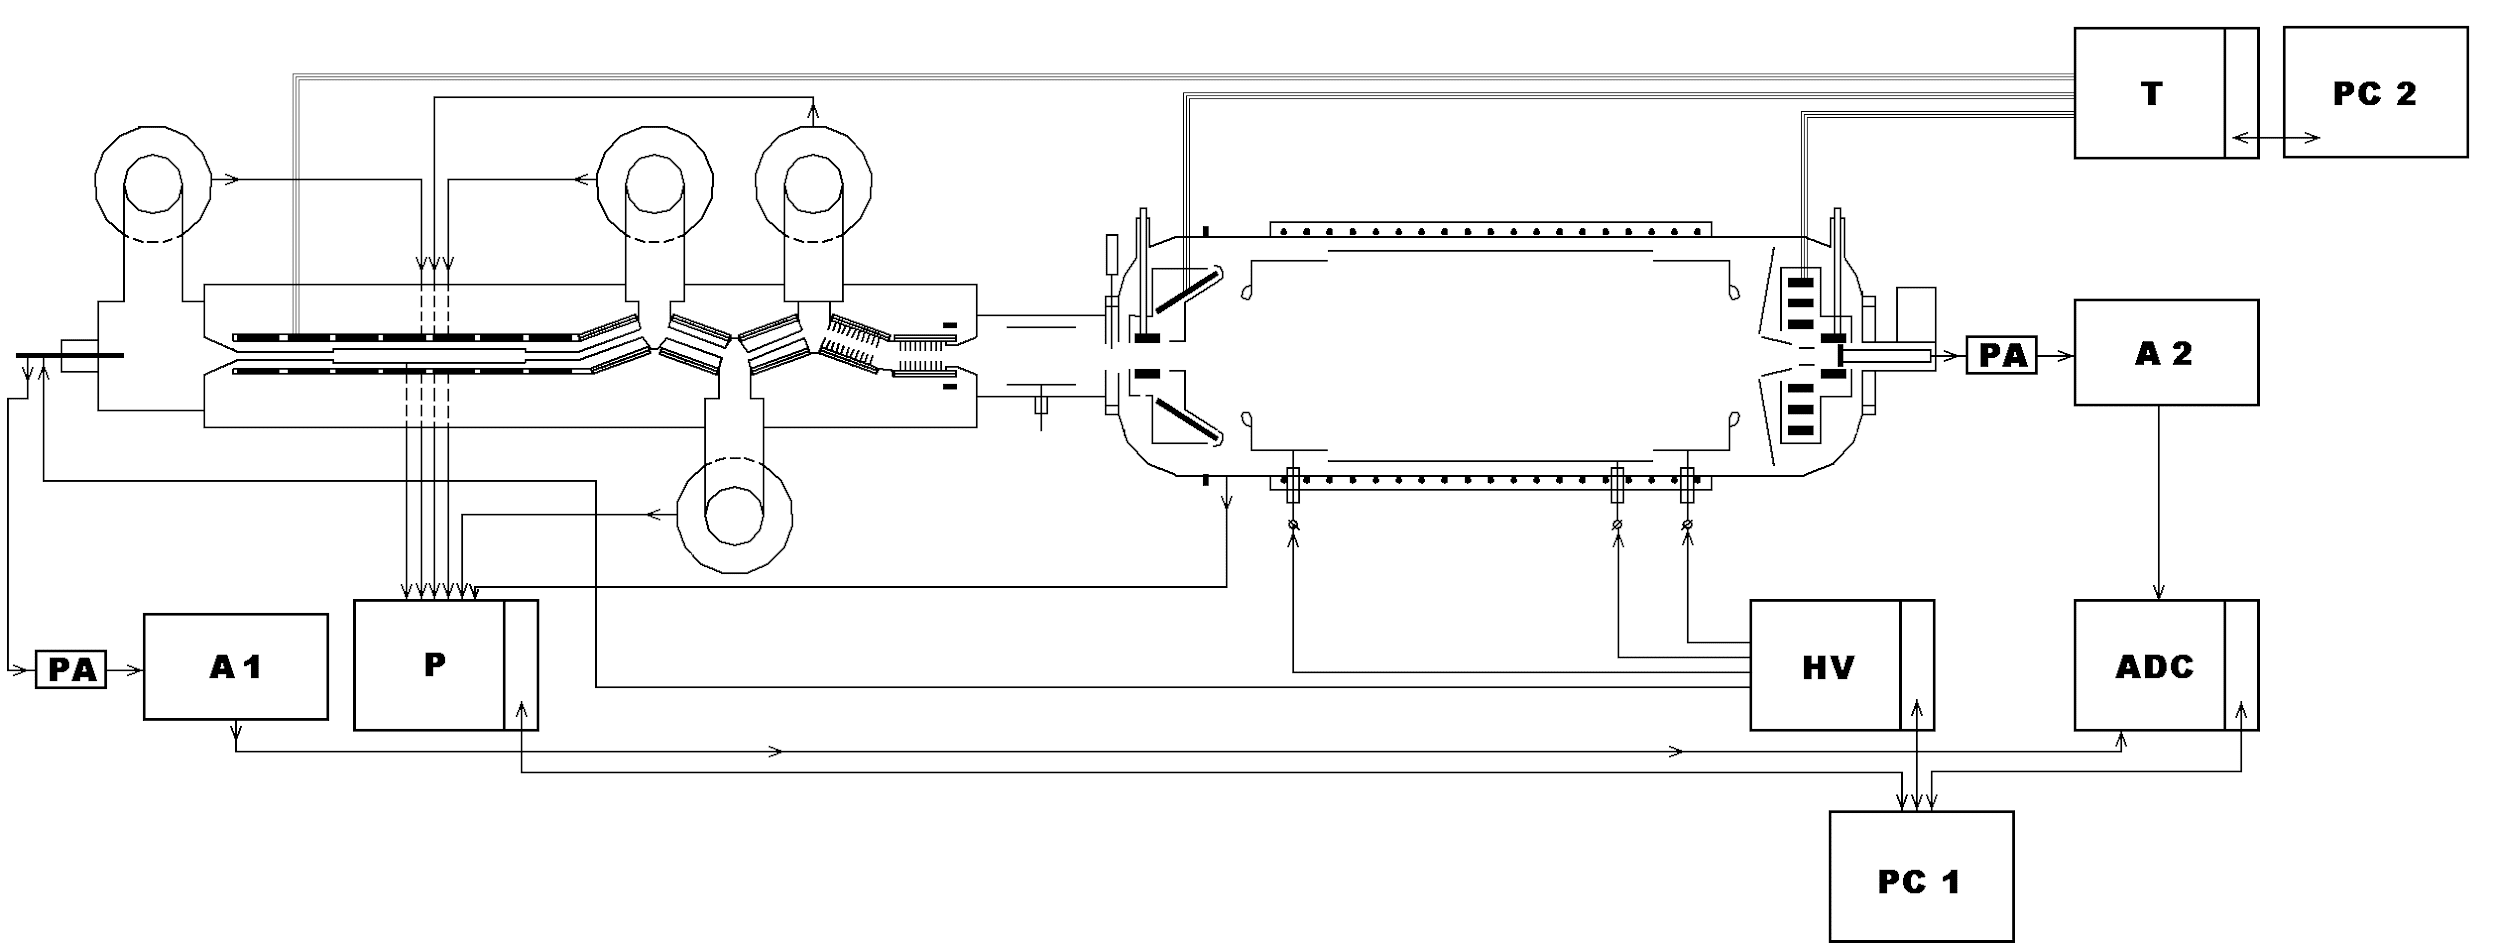
\includegraphics[width = 0.99\textwidth]{img/nu_mass_setup/acquisition-old.png}
    \caption{Схема исходной системы сбора данных. Обозначения: PA – предварительные усилители, A1, А2 – крейты аналоговой обработки сигнала (NIM), ADC – крейт оцифровки сигнала, HV – высоковольтная система, P – крейт оцифровки давлений, T – крейт измерения температур, PC 1, PC 2 – персональные компьютеры.}
    \label{fig:numass-acquisition-old}
\end{figure}

Далее в работе мы будем касаться только компоненты управления высоким напряжением (крейт HV и подключенная к нему аппаратная составляющая) и системы регистрации событий на детекторе (крейты A2, ADC). С точки зрения этих компонент, типичный сценарий набора данных на установке состоит из последовательных наборов событий с детектора за фиксированный отрезок времени при фиксированном напряжении спектрометра (точек). Точки отличаются друг от друга величиной запирающего напряжения и, в случае большой разницы в скоростях счета, временем набора. На рис \ref{fig:numass-acq-graph} показана блок схема цикла набора.

Помимо активного управления  во время набора измерений производится непрерывная запись и мониторинг данных медленного контроля, таких как давления ртутных насосов, температуры элементов криогенной части системы и значения магнитных полей.

\begin{figure}
  \centering
  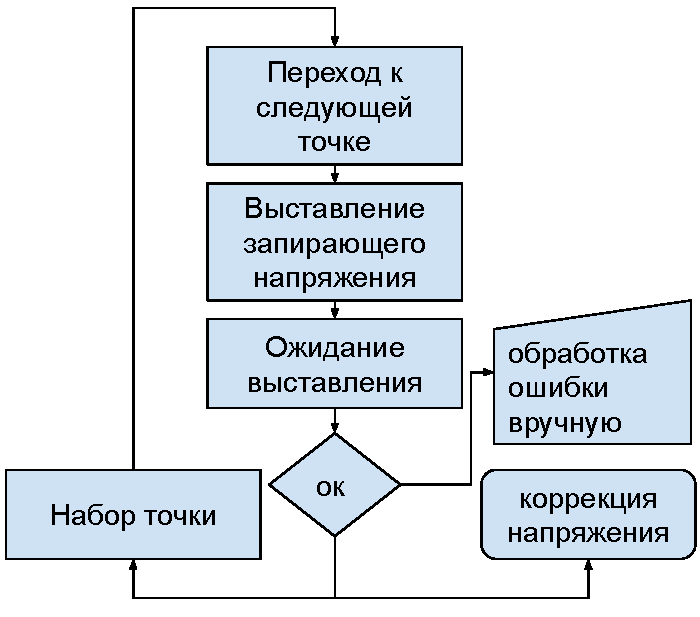
\includegraphics[height = 0.4\textwidth]{img/nu_mass_setup/acq_graph.pdf}
    \caption{Блок-схема набора по сценарию.}
    \label{fig:numass-acq-graph}
\end{figure}

\section{Аппаратная составляющая системы сбора данных}

Созданная в процессе работы система сбора данных установки Троицк ню-масс аппаратно опирается на готовые наработки, использующиеся на установке с 1993 года. Конкретно, система использует электронику установленную в детекторной части установки и электронику, отвечающую за работу высоковольтной стойки. Для упрощения понимания работы модернизированной системы сбора данных, которая будет изложена в последующих главах, опишем кратко устройство и принцип работы этих двух компонент установки.

\subsection{Система регистраций событий детектора}

При создании аппаратного комплекса, отвечающего за набор регистрируемых детектором событий, которая впоследствии стала использоваться в эксперименте <<Троицк ню-масс>> закладывалась необходимость регистрации событий в большом диапазоне скоростей счета, границы которого отличаются на шесть порядков - от нескольких килогерц до единиц милигерц. При этом, т.к. предполагалось измерять среднюю скорость счета регистрируемых событий - дополнительным требованием для создаваемой системы стала необходимость исключения пропусков импульсов при наборе.

Установка <<Троицк ню-масс>> использует в качестве основного регистрирующего детектора изготовленный в ПИЯФ по специальному заказу плоский Si(Li) детектор с диаметром чувствительной области 17 мм, ёмкостью порядка 15 пФ со слоем золота 20 мкг/см2, охлаждаемый до температуры жидкого азота \todo{в последних сеансах другой детектор, уточни у Влада или Сергея}. Приходящий на детектор сигнал импульса попадает в предварительный усилитель ПУМА-73, головной каскад которого расположен рядом с детектором и тоже охлаждается; остальная часть предусилителя, в целях упрощения эксплуатации без нарушения вакуума, вынесена на 1 м от детектора. Из предварительного усилителя сигнал попадает на основной усилитель ORTEC 572, обрабатывающий импульсы а методом однократного дифференцирования и интегрирования с одинаковыми постоянными и имеющим время формирования - 0.5 мкс. Далее идет оцифровка сигнала, которая осуществляется 12-разрядным спектрометрическим аналого-цифровым преобразователем типа ADC-4K производства ПИЯФ. АЦП работает по принципу поразрядного взвешивания с динамическим выравниванием и имеет постоянное время преобразования составляющее 3.91 мкс. Для сохранения параметров регистрируемых импульсов применяется специальный блок MADC (модуль буферной памяти с фиксацией времени прихода каждого события), разработанный и изготовленный по специальному заказу в ЛВЭ ОИЯИ (г. Дубна), и выполненный в стандарте КАМАК. MADC имеет шаг оцифровки времени от 50 до 200 нс в зависимости от длительности набора событий. Емкость модуля составляет 1.5 Мегабайта, которой хватает на запись 256К событий - при записи каждое событие занимает 48 байт: 12 на амплитуду, 28 на время прихода и 8 - на служебную информацию.
Взаимодействие между АЦП и MADC можно описать следующей последовательностью действий:
\begin{itemize}
    \item При превышении входным сигналом установленного порога срабатывает     формирователь, открывающий вход АЦП. Вход открывается на фиксированный отрезок времени соответствующий времени  формирования сигнала с небольшим запасом, при котором попадающий сигнал будет заведомо содержать пик импульса. В дополнение срабатывание формирователя также приводит к инкрементации показателя счетчика  4СчБ.
    \item После открытия входа АЦП начинается непрерывный поиск пика импульса, после нахождения которого начинается преобразование.
    \item В момент начала преобразования АЦП подаёт сигнал в MADC, который записывает в текущее событие метку времени и ожидает завершение преобразования. В процессе преобразования сигнала вход АЦП автоматически блокируется.
    \item После завершения преобразования, которое занимает 3.91 мкс, АЦП выставляет полученный код на внешнюю шину (4) и подает сигнал строба. MADC по стробу считывает выставленный код и записывает его ко времени, которое было установлено на предыдущем шаге. После, MADC выдает сигнал подтверждения для АЦП. Запись амплитуды события в память суммарно занимает 100 нс.
    \item Система готова к приему и обработке следующего события.
\end{itemize}
Описанная схема набора изображена на временной диаграмме на рисунке \ref{fig:numass-madc-timeline}; на рис \ref{fig:numass-madc-signal-processing} приведена полная схема аппаратной оцифровки.

\begin{figure}
  \centering
  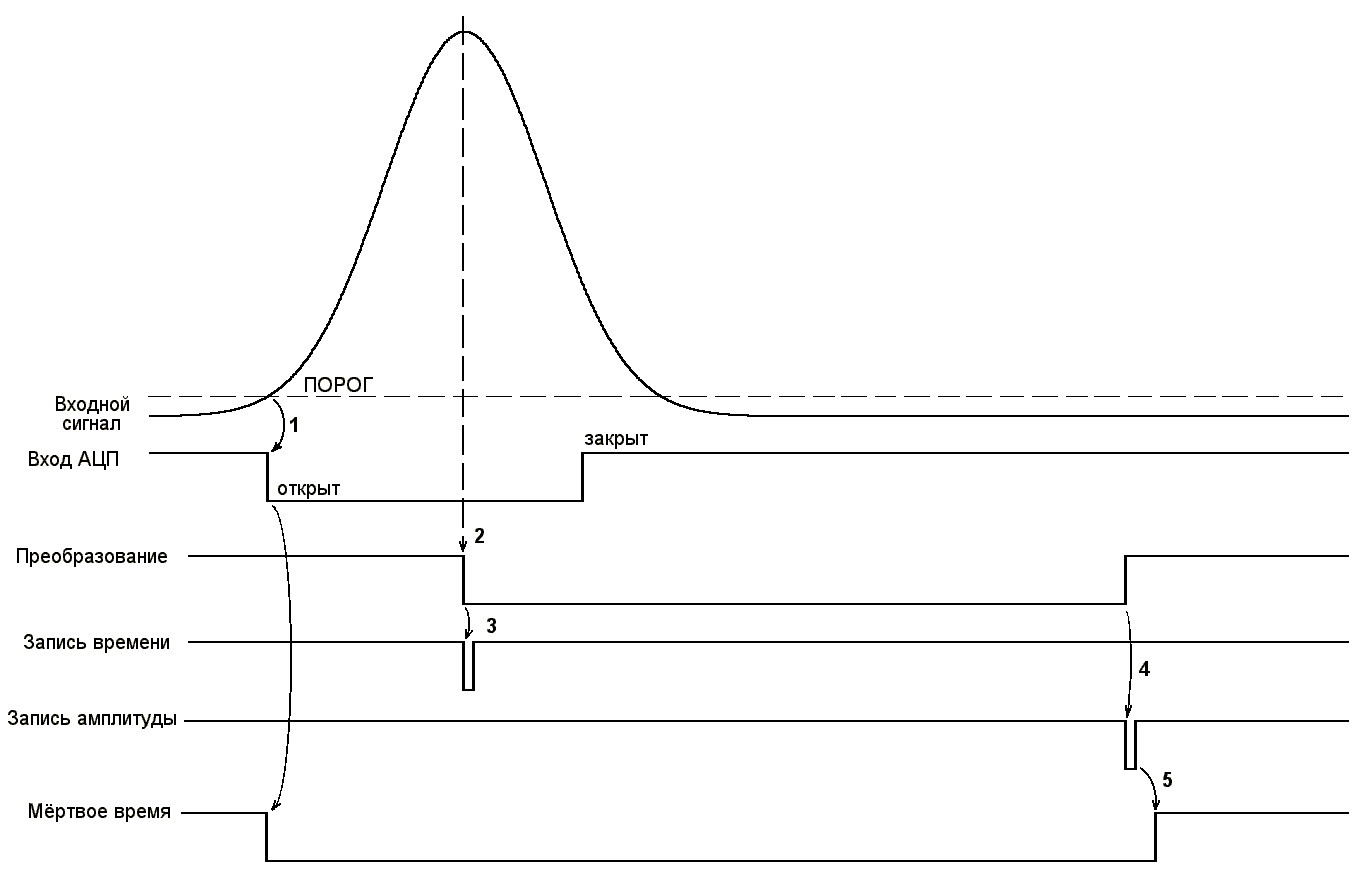
\includegraphics[width = 0.98\textwidth]{img/nu_mass_setup/madc_timeline.png}
    \caption{Оцифровка и запись события в MADC.}
    \label{fig:numass-madc-timeline}
\end{figure}

\begin{figure}
  \centering
  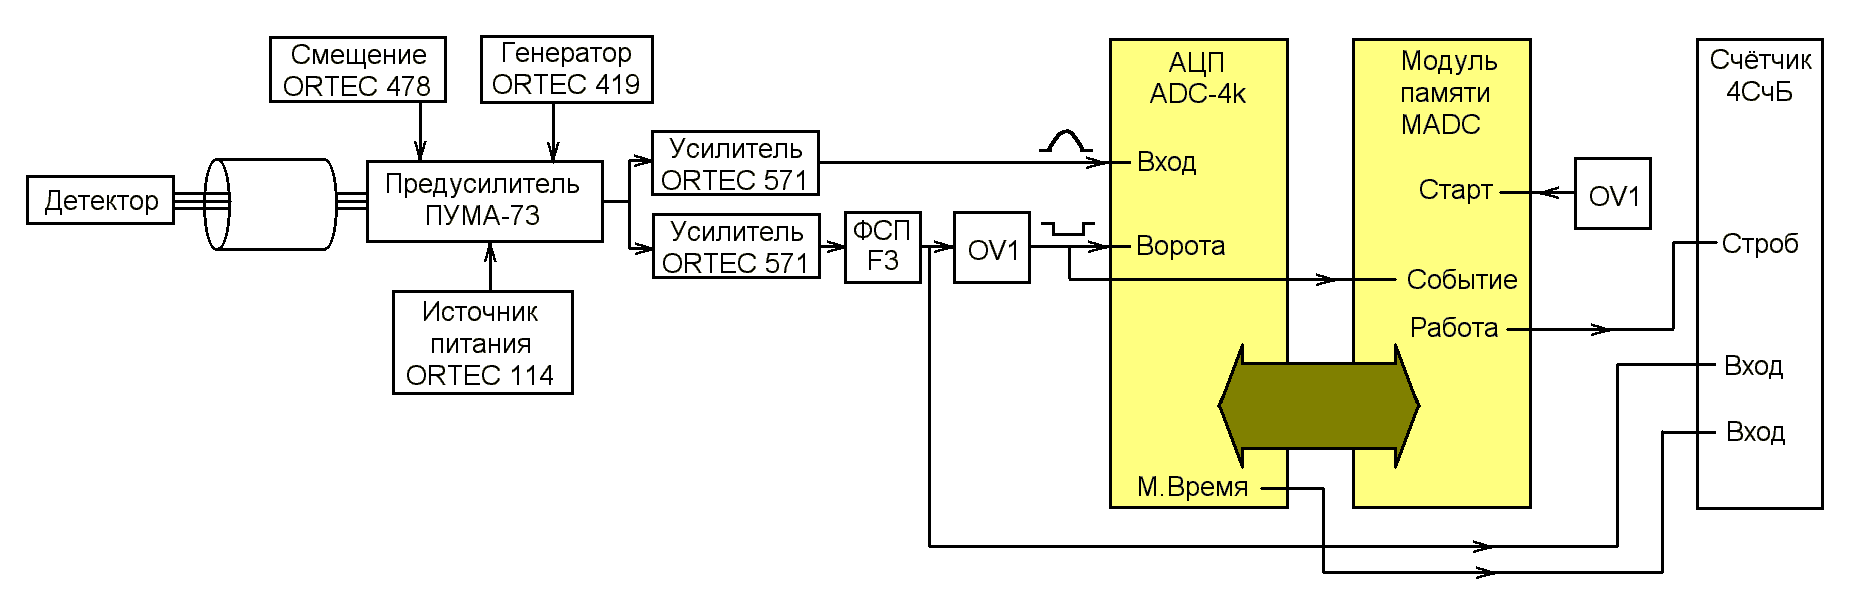
\includegraphics[width = 0.98\textwidth]{img/nu_mass_setup/madc_signal_processing.png}
    \caption{Аппаратная обработка сигнала детектора.}
    \label{fig:numass-madc-signal-processing}
\end{figure}

Мёртвое время системы сбора отсчитывается от момента открытия входа АЦП до конца     цикла записи в память MADC и составляет 6.0 мкс.

Для обхода аппаратных ограничений на пропускную способность транспортной шины КАМАК, АЦП и MADC соединены между собой внешней шиной. Такая конфигурация позволяет добиться быстродействия, недостижимого ни на одном из индустриальных стандартов, используемых во время проектирования системы.

\subsection{Система управления запирающим напряжением}

Аппаратный комплекс, осуществляющий управление и контроль напряжения спектрометра вынесен в отдельную стойку, находящуюся в основании спектрометра. Основными элементами высоковольтной системы являются:
\begin{itemize}
    \item Прецизионный цифроаналоговый преобразователь В1-13 (прибор для проверки вольтметров); в системе сбора данных этот прибор используется для установки опорного напряжения всей системы стабилизации. С помощью изменения опорного напряжения происходит задания величины задерживающего потенциала спектрометра. Управление устройством осуществляется через установленный в стойку КАМАК с помощью 24‑разрядного параллельного регистра типа POLON 350. Один канал модуля осуществляет запись в ЦАП управляющих команд, другой задает величину напряжения
    \item Управляемый линейный высоковольтный преобразователь HV-30, изготовленный по заказу в Обнинске. Преобразователь имеет коэффициент увеличения входного напряжения порядка 5500 раз. Помимо аналогового входа, через который с помощью ЦАП В1-13 задается опорное напряжения, устройство имеет дополнительный разъем с интерфейсом взаимодействия RS-485, с помощью которого можно проводить тонкую настройку напряжения в пределах 1 кВ.
    \item Делители напряжения с коэффициентом 1:2026. Применяются для считывания установленного преобразователем HV-30 напряжения с целью его контроля.
    \item Прецизионные вольтметры Solarton 7061, которые с помощью аналогового измерительного коммутатора 164 соединяются с делителями и считывают с них напряжение. Вольтметры имеют возможность программного управления через последовательный интерфейс RS-232.
    \item Стабилизирующий модуль, принцип действия которого будет описан ниже.
\end{itemize}

Схема работы высоковольтной стойке изображена на рисунке \ref{fig:numass-hv-scheme}. Источниками питания для системы являются магистраль крейта КАМАК и два дополнительных источника типа ТЕС‑14, которые управляются с помощью ЦАП В1-13 и встроенный в блоки интерфейс RS-232.

\begin{figure}
  \centering
  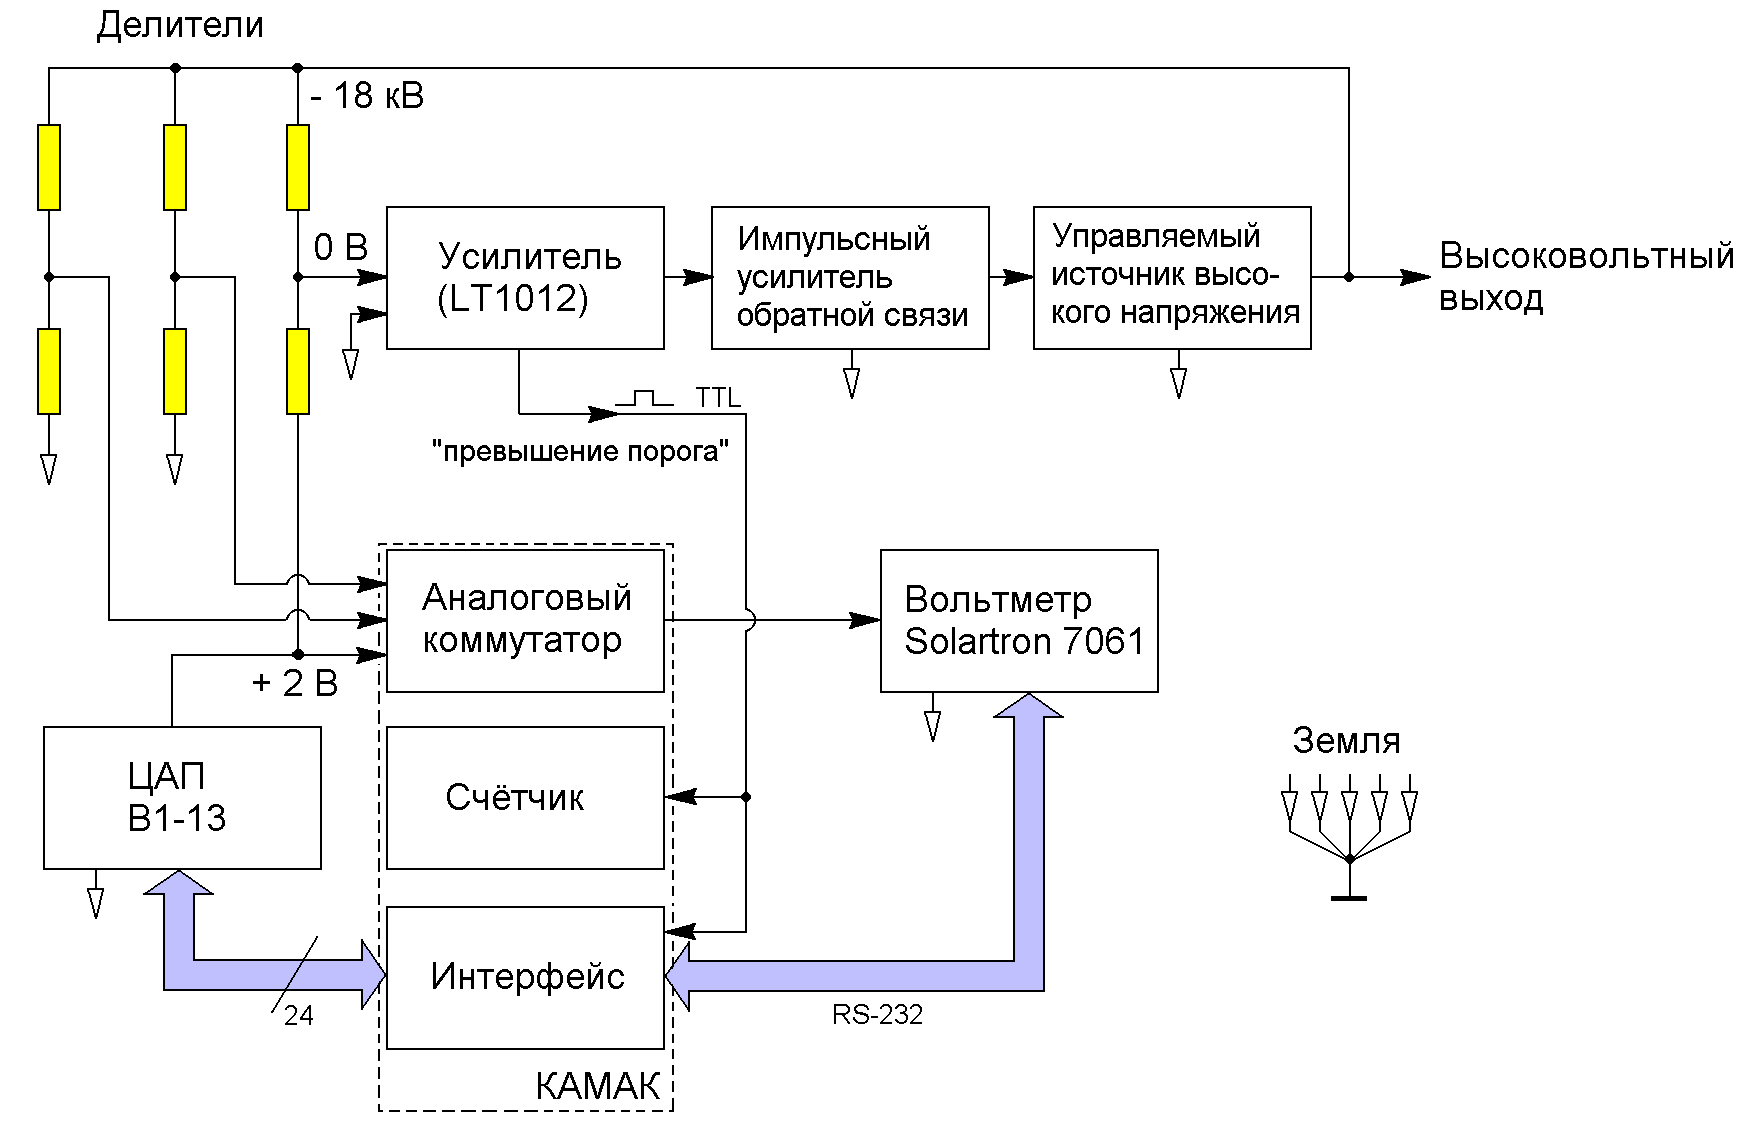
\includegraphics[width = 0.98\textwidth]{img/nu_mass_setup/hv_scheme.png}
    \caption{Схема работы высоковольтной стойки.}
    \label{fig:numass-hv-scheme}
\end{figure}

Схему кратковременной аппаратной стабилизации высоковольтного напряжения можно представить в виде следующей последовательности действий:
\begin{enumerate}
    \item Установленное высоковольтное напряжение (отрицательное) и опорное напряжение с ЦАПа (положительное) подаются на два плеча делителя. На средней точке делителя должен установиться нулевой потенциал, если эти два напряжения соответствуют друг другу.
    \item Потенциал средней точки делителя усиливается операционным усилителем с очень малым входным током (LT 1012). Тут же стоят и компараторы, следящие за отклонениями высоковольтного напряжения («быстрая» схема сравнения).
    \item Усиленный сигнал подаётся на вход интегрирующего импульсного усилителя обратной связи. Вход этого усилителя открывается на малое время и сигнал рассогласования попадает на интегратор, увеличивая либо уменьшая управляющее напряжение на небольшую величину. Таким образом удаётся избежать «раскачки» довольно инерционной системы управления высоковольтным напряжением и сделать ее нечувствительной к кратковременным помехам и пробоям (см. рис. \ref{fig:numass-hv-stabilizer-scheme}).
    \item Управляющий сигнал попадает на вход линейного высоковольтного преобразователя напряжения.
\end{enumerate}

\begin{figure}
  \centering
  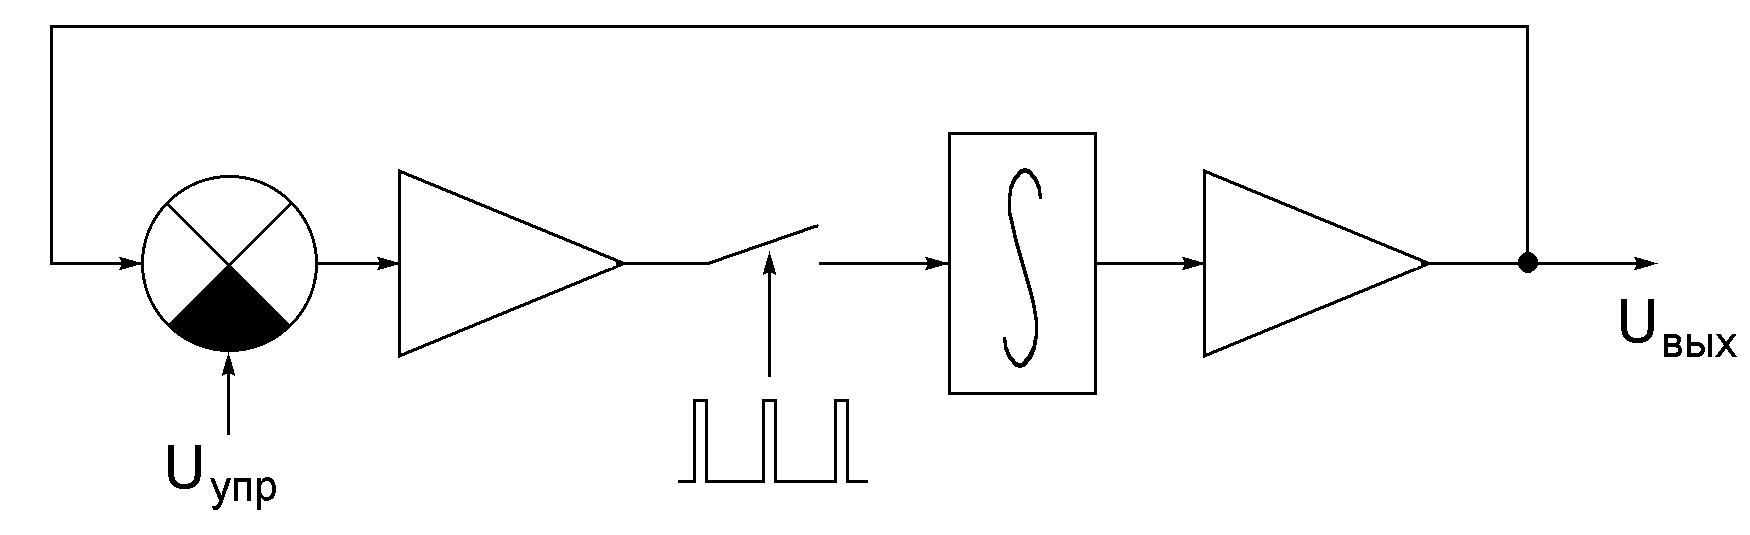
\includegraphics[width = 0.98\textwidth]{img/nu_mass_setup/hv_stabilizer_scheme.png}
    \caption{Схема стабилизатора высокого напряжения.}
    \label{fig:numass-hv-stabilizer-scheme}
\end{figure}

Описанная схема позволяет устранить кратковременные скачки в системе, однако при долгосрочных измерениях (для времен измерений порядка 10 часов и более) выставленное напряжение все равно будет “уплывать” от заданного. Устранение подобных отклонений в высоковольтной стойке ложится на алгоритмы управляющего компьютера. Аппаратно, стойка позволяет считывать напряжение с делителей с помощью вольтметров и задавать через ЦАП и  RS-232 интерфейс преобразователя напряжения. Это позволяет при постоянном мониторинге показаний вольтметров вычислять отклонения от желаемых значений и вносить их в устанавливаемое напряжение. Т.к. преобразователь имеет 2 входа для установки напряжения, один их них (аналоговый) используется для установки полного значения а другой (RS-232) для внесения коррекций, обеспечивающих долгосрочную стабильность.

\todo[inline]{Надо бы добавить небольшой кусок про то, почему вообще надо стабилизировать напряжение}

\chapter{Архитектура системы сбора}

\section{Формат хранения и передачи данных}

Во время продумывания новой архитектуры системы сбора установки <<Троицк ню-масс>> и с учетом предыдущего негативного опыта потери данных вследствие ненадежности или неудобности формата хранения (например разбиения на несколько файлов логически атомарной единицы данных, потеря описания формата данных, изменения формата в процессе набора и др) было решено выработать продуманный единый формат хранения и передачи данных и использовать его в новой системе.

Для формата были сформулированы следующие требования:
\begin{enumerate}
    \item Формат должен быть максимально гибким. Его использование потенциально не должно ограничиваться только установкой <<Троицк ню-масс>> - должна быть возможность имплементации на другие установки и фреймворки.
    \item Передаваемые и сохраняемые на жесткий диск пакеты данных должны иметь одинаковый формат. Различие форматов ведет к ненужному усложнению для понимания работы системы в то же время не создавая значительного преимущества в производительности.
    \item Пакет данных должен иметь возможность содержания текстовых полей (метаданных) и бинарных полей (набранные данные). Оба вида данных в пакете опциональны. Типичная логически цельная единица данных для экспериментальной физики частиц практически всегда представляет из себя метаданные, содержащие информацию о параметрах набора и собственно сами набранные данные, которые чаще всего целесообразно хранить в бинарном виде ввиду их объема. С учетом этого описанное требование выглядит естественным для специфики данных. Объединения двух видов данных в один неделимый пакет усложняет потерю части набранных данных при дальнейших манипуляциях с ними.
    \item Метаданные пакета должны читаться без необходимости прочтения всего пакета. Выполнение этого требования обеспечивает возможность быстрого предварительного анализа, фильтрации и индексации набранных данных.
    \item Содержание метаданных пакета должно иметь человекочитаемый формат. Содержание пакета должно быть понятно при работе с пакетом через текстовый редактор. В этом случае пакет можно будет открыть без дополнительного ПО и в дальнейшем понять, какое ПО необходимо для полноценной обработки. Также облегчается отладка и понимание работы системы.
    \item Протоколом передачи сообщений должен служить TCP/IP. Это обеспечит относительно простое встраивание в установку в силу доступности и дешевизны соответствующего оборудования и возможности протягивания кабелей на длинные дистанции. Современное оборудование позволяет построить сеть с пропускной способностью до 100 Гбит/с, что покрывает практически все потенциальные требования для экспериментов. С другой стороны наличие огромного числа имплементаций библиотек для работы с протоколом практически для всех языков обеспечивает простоту разработки модулей сбора данных.
    \item Хранение данных на жестком диске должно реализовываться средствами файловой системы и быть имплементировано в виде древовидной структуры, состоящей из папок и файлов. Для обеспечения чистоты и объективности результатов анализа, необходимо всегда опираться только на исходные данные, полученные напрямую с установки. Поэтому собранные и сохраненные в процессе эксперимента пакеты данных должны быть принципиально неизменяемыми. В случае, если для данных требуется коррекция (например перекалибровка для отдельных датасетов) она должна быть выполнена в виде отдельного файла, задающего мутацию данных. Такая специфика делает хранение данных в привычных форматах таких как реляционные базы данных не оптимальным ввиду усложнения работы с ними и неиспользования их сильных сторон из-за иммутабельности. Хранение в виде древовидной структуры в файловой системе достаточно и обеспечивает наглядность при работе с данными.
\end{enumerate}

На момент разработки из известных и реализованных форматов, под требования частично подходил только формат Http-multipart, однако от его использования было решено отказаться, т.к. сам формат не смотря на продолжительное существование не обрел популярности. В частности для него нет работающего парсера на Python, способного десериализовать пакеты, содержащие бинарные поля (однако есть временное решение в виде коммита\cite{multipart-fix}). Кроме того для хранения пакета используются несколько файлов, что затрудняет процесс обработки и хранения данных а передача пакетов требует использования http, который в общем случае не предназначен для передачи бинарных данных и для нашей задачи является излишней настройкой на протокол TCP/IP.

Ввиду отсутствия на момент разработки готовых форматов, удовлетворяющих всем сформулированным требованиям было принято решение о разработке собственного формата для системы хранения. При этом, для обеспечения долговечности и упрощения разработки, реализации все равно максимально использовали уже существующие форматы и их реализации.

\subsection{Формат DataForge Envelope}

В качестве формата хранения и передачи данных используется формат dataforge-envelope из фреймворка DataForge\cite{dataforge}. Фреймворк DataForge позволяет обрабатывать данные в области экспериментальной физики частиц. В основе архитектуры лежит data-driven принцип - любая обработка представляется как граф математических преобразований исходных данных. Каждый узел графа содержит правила обработки, в случае успешной обработки - кэш данных с результатом. Все данные фреймворка хранятся в формате dataforge-envelope. Рассмотрим подробнее этот формат.

\begin{figure}
  \centering
  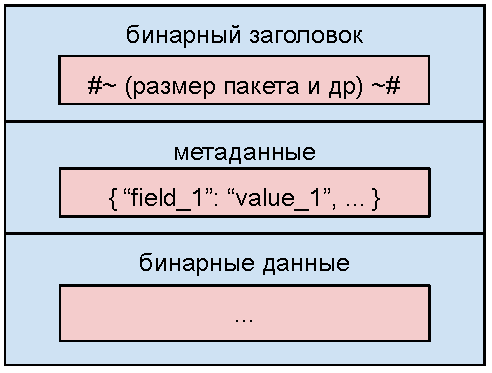
\includegraphics[width = 0.4\textwidth]{img/dataforge/message.pdf}
    \caption{Схема стабилизатора высокого напряжения.}
    \label{fig:datafoge-message}
\end{figure}

На рисунке \ref{fig:datafoge-message} схематично изображена структура пакета.
В использующемся протоколе TCP/IP передача данных происходит через бинарный поток. При этом фактически данные передаются фрагментированными пакетами. Фрагментация обуславливается не логической связностью передаваемых данных а передаваемым объемом и общим состоянием сети. TCP/IP не имеет в себе функционала логического объединения данных а обеспечивает только правильность последовательности прихода пакетов. Поэтому при передачи пакетов больших объемов на модуль обработки ложится задача выделения и склеивания данных из общего потока. Существует 2 способа объединения данных:
\begin{enumerate}
    \item Объединение с помощью открывающих и замыкающих специальных последовательностей символов. В этом случае перед началом пакета вписывается заголовок определяющий начало пакета далее записывается уникальная последовательность бинарных символов определяющая начало содержимого пакета. В конец пакета записывается та же последовательность. Эта последовательность не должна встречаться в самом пакете. Т.к. для каждого пакета может быть определена своя последовательность - это ограничение вполне выполнимо. Здесь последовательность для наглядности стоит рассматривать как бинарный аналог обычных скобок. Такой способ объединения реализован например в http-multipart. Из достоинств такого подхода стоит рассмотреть удобство использования при составлении пакетов вручную.
    \item Объединение с помощью заголовка фиксированной длины, содержащего размер содержимого пакета. В этом способе после чтения заголовка, в буфер считывается последующие байты в количестве, указанном в заголовке. Такой подход значительно проще в реализации, т.к. требует меньше шагов при парсинге, однако создание пакетов в ручном режиме сильно затрудняется, т.к. требует подсчета размера содержимого.
\end{enumerate}
Формат dataforge-envelope использует второй подход в силу его простоты. Для обеспечения возможности создания пакетов вручную в формате предусмотрено исключение, которое будет описано в последующих подразделах. Заголовком, содержащим размер пакета служит <<бинарный заголовок>>, изображенный на схеме. Т.к. пакет предусматривает содержание текстовых и бинарных данных, в заголовок записываются 2 числа, соответствующие размерам этих частей. Общая длина пакета получается суммированием этих чисел плюс константным размером разделителей, присутствующих в пакете.

После бинарного заголовка в пакете dataforge-envelope идет часть “метаданные”, содержащая текстовые метаданные пакета. В качестве формата метаданных потенциально может выступать любой язык разметки, реализующий древовидную структуру. Сам тип языка разметки указывается в бинарном заголовке. На момент написания были реализованы языки XML и JSON, при этом на установке Троицк ню-масс в основном используется JSON. Dataforge-envelope не накладывает ограничений на содержание метаданных, это оставляется на усмотрение разработчика системы сбора и анализа.

Замыкает пакет часть “бинарные данные”, содержащая бинарные данные. Формат пакета также не накладывает ограничений на формат бинарных данных в силу их разнообразия. Предполагается, что способ парсинга формата бинарных данных будет однозначно определяться метаданными пакета.

Все 3 части пакета dataforge-envelope разделяются спец последовательностью символов \colorbox{Gainsboro!60!Lavender}{\textbackslash r \textbackslash n}.

Из достоинств формата можно выделить:
\begin{itemize}
    \item Возможность передачи пакетов низкоуровневыми протоколами связи по типу TCP/IP. Также есть возможность хранения пакетов без изменений средствами файловой системы.
    \item Возможность создания вложенных пакетов.
    \item При использовании совместно с файловой системой формат позволяет использовать каскадные поля метаданных для вложенных подгрупп пакетов.
\end{itemize}
К недостаткам можно отнести:
\begin{itemize}
    \item Затрудненность создания пакета вручную. Однако, как уже было сказано ранее, формат предполагает некоторое исключение, облегчающие данный процесс.
    \item Вольность задания метаданных и формата бинарных данных. Параметры должны быть ограничены внешними правилами. Этот недостаток появляется вследствие большого потенциального разнообразия данных и принципиально не может быть исправлен.
\end{itemize}
Пример сообщения, содержащего информацию о напряжении на спектрометре во время набора, открытый через текстовый редактор nano:
\begin{lstlisting}[caption={Пример сообщения в формате Dataforge Envelope.}, captionpos=b]
#!^@^A@^@Z^UH'^@^A^@^@^@^@^@'^@^@^B^A^@^@''!#
{
    "format_description": "https://...$",
    "programm_revision": "1.1.1-75-gd67324e",
    "type": "voltage"
}

2017-11-22T11:15:01 1 15999.9
2017-11-22T11:15:05 1 16000
2017-11-22T11:15:09 1 16000
2017-11-22T11:15:13 1 16000
...
2017-11-22T12:51:41 1 14900
2017-11-22T12:51:45 1 14900
2017-11-22T12:51:49 1 14900
\end{lstlisting}

\subsubsection{Версии форматов}
В формат протокола dataforge-envelope в процессе разработки системы сбора данных вносились исправления, призванные улучшить его и убрать оказавшиеся ненужными элементы. На данный момент существует 3 версии протокола. Т.к. система сбора данных в силу инертности разработки использует все версии, опишем их. 

Версии отличаются друг от друга только бинарным заголовком пакета. Поэтому с помощью регулярных выражений или простого сравнения спецсимволов можно однозначно определить к какой версии пакет относится.

\paragraph{0x14000}
Для всех версий бинарный заголовок ограничивается открывающей и замыкающей последовательностью спецсимволов длиной 2. Тип сообщения (внутренняя версия) определяется 4 байтами, идущими после открывающей последовательности. В последних версиях это 4 текстовых символа. Однако в первых версиях эти символы были бинарными. Формат 0x14000 - первая версия протокола. Название соответствует 4 бинарным символам типа в hex кодировке.

Бинарный заголовок имеет размер 30 байт. Структура заголовка соответсвует таблице \ref{tab:01400-binary-structure}.
\begin{table}
    \centering
    \begin{tabular}{|l|l|l|}
    \hline
    Байты & Значение & Описание \\
    \hline
    0-2 & \#! & Открывающая последовательность символов \\
    \hline
    2-6 & unsigned int32 & Тип сообщения. Статичное значение 0x14000 \\
    \hline
    6-10 & unsigned int32 & Время создания сообщения (формат неопределен) \\
    \hline
    10-14 & unsigned int32 & Тип метаданных \\
    \hline
    14-18 & unsigned int32 & Длина метаданных в байтах \\
    \hline
    18-22 & unsigned int32 & Тип бинарных данных \\
    \hline
    22-26 & unsigned int32 & Размер бинарных данных в байтах \\
    \hline
    26-30 & !\#\textbackslash  r\textbackslash n & Закрывающая последовательность символов \\
    \hline
    \end{tabular}
    \caption{Структура бинарного заголовка версии 0x14000.}
    \label{tab:01400-binary-structure}
\end{table}

Типы метаданных:
\begin{itemize}
    \item "UNDEFINED\_METATYPE": 0x00000000 - неопределенный формат метаданных
    \item "JSON\_METATYPE": 0x00010000 - метаданные в формате JSON
    \item "QDATASTREAM\_METATYPE": 0x00010007 - метаданные в формате QDataStream (встроенный в Qt бинарный парсер)
\end{itemize}
Типы бинарных данных:
\begin{itemize}
    \item "UNDEFINED\_BINARY": 0x00000000 - неопределенный формат
    \item "POINT\_DIRECT\_BINARY": 0x00000100 - массив событий время-амплитуда
    \item "POINT\_QDATASTREAM\_BINARY": 0x00000107 - массив событий время-амплитуда, сериализованный QDataStream
    \item "HV\_BINARY": 0x00000200
    \item "HV\_TEXT\_BINARY": 0x00000201
\end{itemize}

\paragraph{DF02}
При работе с данными оказалось, что формат 0x14000 имеет излишние поля в бинарном заголовке: в частности оказались неиспользуемыми поля прихода пакета и формата бинарных данных - вся необходимая информация содержалась в метаданных пакета. В дополнение открывающая последовательность спецсимволов имела коллизии с форматом shebang\cite{wiki:Shebang_Unix}. К тому же при просмотре файлов через текстовый редактор возникали трудности с прочтением полей бинарного заголовка.

Впоследствии была разработана версия <<DF02>> с описанной в таблице \ref{tab:df02-binary-structure} структурой полей.

\begin{table}
    \centering
    \begin{tabular}{|l|l|l|}
        \hline
        Байты & Значение & Описание \\
        \hline
        0-2 & \#\textasciitilde & Открывающая последовательность символов \\
        \hline
        2-6 & unsigned int32 & Тип сообщения. DF02 == 0x44463032 \\
        \hline
        6-8 & unsigned int16 & Тип метаданных \\
        \hline
        8-12 & unsigned int32 & Длина метаданных в байтах \\
        \hline
        12-16 & unsigned int32 & Длина бинарных данных в байтах \\
        \hline
        16-20 & \textasciitilde\#\textbackslash r\textbackslash n” & Закрывающая последовательность символов \\
        \hline
    \end{tabular} 
    \caption{Структура бинарного заголовка версии DF02.}
    \label{tab:df02-binary-structure}
\end{table}

Типы метаданных:
\begin{itemize}
    \item "UNDEFINED\_METATYPE": 0x00000000 - неопределенный формат метаданных
    \item "JSON\_METATYPE": "JS" - метаданные в формате JSON
    \item "XML\_METATYPE": "XM" - метаданные в формате XML
\end{itemize}

\paragraph{DFTL}
Для отладки системы и манипулирования в ручном режиме формат dataforge-envelope предусматривает специальную версию только для файлов. В ней в бинарном заголовке не указываются размеры пакетов, а сами части разделяются последовательностями спецсимволов:
\begin{itemize}
    \item \#\textasciitilde DFTL\textasciitilde\# - для начала пакета
    \item \#\textasciitilde META\textasciitilde\# - для части, содержащей метаданные
    \item \#\textasciitilde DATA\textasciitilde\# - для части, содержащей бинарные данные
\end{itemize}
В данной версии флагом завершения пакета является конец файла. Таким образом версия DFTL позволяет простым образом создавать валидные пакеты с помощью текстового редактора.

\subsubsection{Типы бинарных данных}
В силу различия сохраняемых данных и по историческим причинам система сбора данных установки Троицк ню-масс использует 3 основных формата бинарных данных для формирования пакетов. Каждый формат имеет свои достоинства и недостатки и подходит для конкретных типов данных. Разберем каждый из этих форматов.

\paragraph{Формат данных MADC}
Данный самодельный бинарный формат, за исключением экономии памяти путем комбинирования чисел в одно поле полностью повторяет формат записи данных старой системы сбора, написанной Задорожным С.В. Структура данных, используемая в формате, в свою очередь повторяет структуру выходных данных, записанных в  MADC с электроники детектора. Бинарные данные формата MADC представляют собой последовательно записанные в бинарном виде события, считываемые с детектора. Формат отдельного события описан в таблице \ref{tab:madc-event-structure}.

\begin{table}
    \centering
    \begin{tabular}{|l|l|l|}
        \hline
        Байты & Значение & Описание \\
        \hline
        0-2 & unsigned int16 & Амплитуда \\
        \hline
        2-6 & unsigned int32 & Относительное время (в единицах MADC) \\
        \hline
        6-7 & bool & Флаг корректности \\
        \hline
    \end{tabular}
    \caption{Формат записи события в формате MADC.}
    \label{tab:madc-event-structure}
\end{table}

Данный формат довольно наивен, однако для своей цели он хорошо подходит и его использование упрощает процесс миграции старой логики набора при модернизации системы сбора.

\paragraph{Текстовый формат}
Для упрощения просмотра, для данных медленного контроля, характеризуется небольшим объемом было решено использовать для записи текстовый формат TSV. Т.к. текст может быть прочитан человеком, при анализе не возникнет трудностей с парсингом данных. Пример бинарных данных в текстовом виде (здесь сохранены показания вольтметра в зависимости от времени; формат хранения времени - ISO):

\begin{lstlisting}[caption={Пример данных, набираемых с вольтметра.}, captionpos=b]
2017-11-22T11:15:01 1 15999.9
2017-11-22T11:15:05 1 16000
2017-11-22T11:15:09 1 16000
2017-11-22T11:15:13 1 16000
\end{lstlisting}

\paragraph{Комбинированный формат}
В процессе обновления электроники детектора и перехода на сбор кадров появилась необходимость в создании единого формата хранения бинарных данных, позволяющего содержать в одном блоке как события в виде амплитуд, так и в виде кадров. Такая необходимость вызвана особенностями обработки кадров - в наборе могут присутствовать сложные кадры, которые затруднительно достоверно преобразовать в амплитуду. Такие кадры предполагается сохранять в том же блоке в необработанном виде.

В качестве основы для формата бинарных данных был выбран Protocol Buffers 3 версии\cite{protobuf}.

Protocol Buffers — протокол сериализации (передачи) структурированных данных, предложенный Google как эффективная бинарная альтернатива текстовому формату XML. Разработчики сообщают, что Protocol Buffers проще, компактнее ( от 3 до 10 раз )  и быстрее ( от 20 до 100 раз ), чем XML. Также для Protobuf существуют готовые библиотеки практически для всех популярных языков.

Комбинированный формат, использующийся на установке Троицк ню-масс на языке Proto может быть записан в форме:

\begin{lstlisting}[language=protobuf3,style=protobuf]
syntax = "proto3";
package Rsh;

message Point {
  message Channel {
    message Block {
        message Event {
              uint64 time = 1; 
              bytes data = 2;
        }
        message Peaks {
              repeated uint64 times = 1;
              repeated uint64 amplitudes = 2;
        }
        uint64 time = 1;
        repeated Event events = 2;
        Peaks peaks = 3;
    }
    uint64 num = 1;
    repeated Block blocks = 2;
  }
  repeated Channel channels = 1;
}
\end{lstlisting}
В данных поканально записаны выделенные из блоков события. События могут быть храниться в обработанном и необработанном видах. Для обработанных событий записываются время и амплитуда, для необработанных - время и кадр. 

Описанная структура дает порядка 24\% оверхеда для обработанных событий и 3\% для необработанных.

\subsubsection{Прозрачная архивация}
С целью уменьшения объема хранимых данных при сохранении возможности прочтения метаданных пакетов в формат dataforge-envelope встроена возможность проведения прозрачной архивации данных с помощью библиотеки zlib.

Соглашение о маркировке сжатых бинарных данных:
\begin{itemize}
    \item В корневой части метаданных должно присутствовать поле "compression" со значением "zlib"
    \item Бинарные данные должны быть сжаты с использованием библиотеки zlib
\end{itemize}

Данные условия автоматически выполняются при формировании пакета с помощью реализации протокола  dataforge-envelope на Python. В ридми репозитория python-df-parser\cite{python-df-parser} есть пример создания пакета с сжатой бинарной частью.

\subsubsection{Структура хранения данных на HDD}
Dataforge-envelope в связке с хранением посредством файловой системы предполагает хранение файлов с выполнением следующих правил:
\begin{enumerate}
    \item Минимальной единицей информации является пакет формата dataforge-envelope, записанный в отдельный файл.
    \item Группы файлов могут быть скомбинированы в одной папке. Для папки предусмотрен специальный файл с названием metadata также имеющий формат dataforge-envelope без бинарных данных и содержащий общие для группы параметры.
    \item Группы также могут быть сгруппированы по средствам объединения в одну папку.
    \item Поле в файле метаданных группы распространяются на все вложенные файлы, если в них нет соответствующего переписанного поля.
\end{enumerate}

Для датасетов, набираемых на установке Троицк ню-масс структура сохраняемых данных реализована по правилам:
\begin{enumerate}
    \item Все данные хранятся в одной корневой папке.
    \item Корневая папка содержит подгруппы с проводимыми экспериментальными сеансами. Названия сеансов совпадают с датой их проведения.
    \item Группа сеанса содержит подгруппы наборов, разделенных логически по параметрам (тестовые, разные стадии напуска трития в установку). Подгруппы называются филами. Название фила устанавливается пользователем.
    \item Группа фила содержит подгруппы, соответствующие набору данных при одинаковом сценарии набора. Эти подгруппы называются сетами. Название сета генерируется автоматически по его номеру.
    \item Сет содержит: \begin{enumerate}
        \item Файлы набора событий при заданном напряжении спектрометра. В названии файла присутствуют основные параметры - время набора и желаемое напряжение на спектрометре.
        \item Файл метаданных сета, содержащий описание, комментарии и возникающие при наборе ошибки.
    \end{enumerate}
\end{enumerate}

\subsubsection{Реализации протокола DataForge-envelope}
Созданные на момент написания реализации протокола указаны в таблице \ref{tab:dataforge-implementations}.

\begin{table}
    \centering
    \begin{tabular}{|l|l|l|l|l|}
    \hline
    Язык & 0x14000 & DF02 & DFTL & zlib \\
    \hline
    C++ (Qt) & + & & & \\
    \hline
    Python & + & + & & + \\
    \hline
    Java & + & + & + & + \\
    \hline
    \end{tabular} 
    \caption{Реализации формата Dataforge Envelope.}
    \label{tab:dataforge-implementations}
\end{table}


\section{Модернизированная система сбора}

При разработке новой системы сбора данных для установки Троицк ню-масс с целью увеличения продолжительности срока службы работы программного комплекса и упрощению поддержки и дальнейшей модернизации были сформулированы следующие паттерны разработки:

\begin{itemize}
    \item Использование микросервисной архитектуры. Каждый самостоятельный, логически полный модуль системы должен быть реализован в виде отдельной программы (сервиса), которая выполняет только свою задачу и взаимодействует с другими модулями системы по TCP/IP протоколу используя стандартизированный формат сообщений. Такой подход инкапсулирует всю работу, связанную со взаимодействием с аппаратной частью в отдельные блоки, которые возможно разрабатывать параллельно и независимо друг от друга. Стандартизированный интерфейс взаимодействия обеспечивает легкость модернизации или замены модулей.
    \item Все сервисы должны иметь режим виртуального устройства. В этом режиме сервис должен запускаться на любом ПК и симулировать реальные ответы при запросе. Выполнение этого требования обеспечивает возможность тестирования отдельных элементов системы без включения всех остальных. Кроме того появляется возможность удаленной разработки комплекса. В случае установки Троицк ню-масс, где в качестве ПК для сервисов используются довольно слабые CCPC7\cite{ccpc7}, возможность разработки не непосредственно на используемой в эксперименте аппаратной части сильно увеличивает скорость разработки.
    \item Каждый сервис должен использовать только необходимую для работы информацию и не требовать дополнительных данных. Это должно максимально изолировать сервисы друг от друга и обеспечить независимость их работы. В процессе эксперимента могут появляться проблемы, такие как например неполадки в сети. При таких проблемах монолитные комплексы не смогут работать. Описанное требование призвано обеспечить возможность работы комплекса в условиях сбоев.
    \item Взаимодействие между сервисами должно обеспечиваться одной главной программой. Эта же программа должна предоставлять пользовательский интерфейс и возможность управления набором. Также, для обеспечения стабильности работы в случае поломки компьютера, программа должна быть мультиплатформенной и \ запускаться на всех ПК. Сформулированное требование вытекает из предыдущего пункта. Описанная программа инкапсулирует в себе все взаимодействие между сервисами т.о. обеспечивая независимость их работы.
    \item В отладочных целях, все сервисы и подпрограммы комплекса должны вести логи работы и сохранять их на жесткий диск. Все ошибки и предупреждения при наборе, в случае их появления, должны быть выведены пользователю.
\end{itemize}

С учетом изложенных требований для новой системы сбора данных была выбрана архитектура, соответствующая схеме на рисунке \ref{fig:numass-new-system}, где:

\begin{itemize}
        \item API сервер модуля высокого напряжения - сервис, находящийся на \ CCPC7 стойки высокого напряжения. Отвечает за установку и коррекцию запирающего напряжения спектрометра.
        \item API сервер модуля детектора - сервис, находящийся на CCPC7 детекторной части установки. Отвечает за включение набора приходящих на детектор событий.
        \item GUI клиента - управляющая программа. Отвечает за запуск и управление сценариями набора данных, мониторингом системы набора и сохранением данных.
        \item Bash скрипты - \ набор скриптов, отвечающих за синхронизацию локальной БД с БД сервера данных.
        \end{itemize}

\begin{figure}
  \centering
  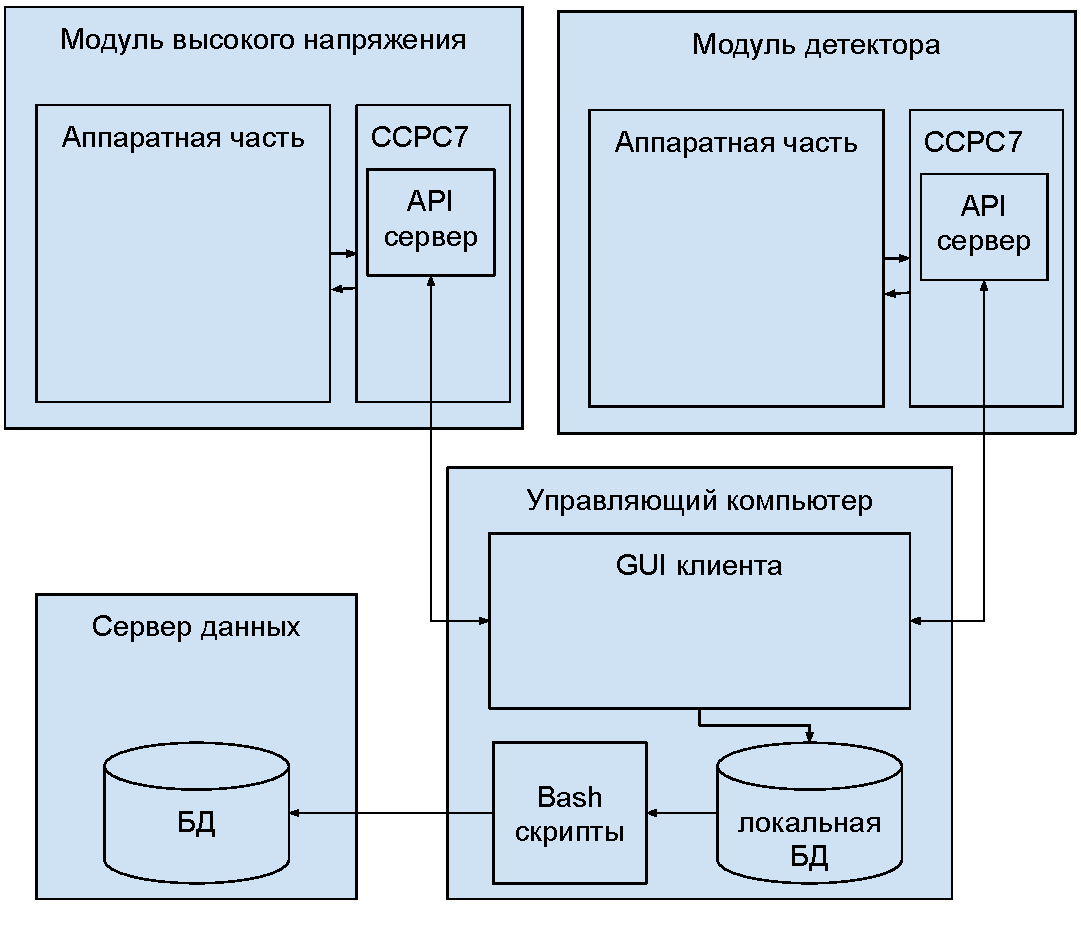
\includegraphics[width = 0.4\textwidth]{img/nu_mass_setup/new_system.pdf}
    \caption{Схема стабилизатора высокого напряжения.
    }
    \label{fig:numass-new-system}
\end{figure}

В качестве фреймворка разработки комплекса выбран Qt. Для устанавливаемых на CCPC7 серверов используется Qt 4.8. Для клиентской части используется версия Qt 5.4. Также используются дополнительные сторонние библиотеки QJson, QCustomPlot и easylogging++. Код хранится в репозитории bibucket единым проектом.


\subsection{Общее для подмодулей комплекса}

\subsubsection{Логирование}

Все модули используют в качестве логгера библиотеку easylogging++. Ее пресет находится в корне проекта в файле easylogging.pri. В конфигурационных файлах сервисов (.pro) логгер подключается командой:

\begin{lstlisting}[language=C++, caption={Подключение пресета common.}, captionpos=b]
include(../common.pri )
\end{lstlisting}

Также в main.cpp сервиса для корректной работы прописаны команды:

\begin{lstlisting}[language=C++, caption={Инициализация пресета common.}, captionpos=b]
#include <easylogging++.h>
#include <common.h>

#ifdef EL_CPP11
    INITIALIZE_EASYLOGGINGPP
#else
    _INITIALIZE_EASYLOGGINGPP
#endif

int main(int argc, char *argv[])
{
    setCodecs();
    initLogging(argc, argv);
    logModes();
\end{lstlisting}

В пресетах common.pri содержится код для:
\begin{itemize}
\item Инициализации логгера.
\item Инициализации временной папки. Создаваемая временная папка в процессе работы сервиса мониторит свой размер и, при превышении порога, удаляет файлы в порядке их создания.
\end{itemize}

\subsubsection{TCP}

В пресете tcp.pri, расположенном в папке tcp находится код для парсинга dataforge-envelope протокола а также коды TCP клиента и API сервера, работающего на этом протоколе. 

Обработка сообщений клиентом и сервером осуществляется с привязки сигналов

\begin{itemize}
    \item receiveMessage - получение сообщение. В привязанном к этому сигналу слоте выполняется код по работе сервиса в соответствии с содержимым входного пакета. 
    \item sendMessage или sendRawMessage - отправка ответа
    \item error - отправка ошибки
\end{itemize}

Такая абстракция позволяет инкапсулировать код по обработке транспортных протоколов в классе-предке и сосредоточиться только на обработке содержимого пакетов.


\subsubsection{Последовательность работы и подключения}
Все сервисы программного комплекса рассчитаны на длительное единоразовое подключение к сокету. После обработки команды сервисы не будут закрывать соединение с клиентом. 

Т.к. логика работы набора данных подразумевает последовательное выполнение команд, в целях упрощения системы все сервисы рассчитаны только на строго последовательное выполнение команд. В случае, если в процессе обработки сервисом очередной команды поступит пакет с новой командой - в ответ на него сервер передаст ошибку :

\begin{lstlisting}[caption={Пример сообщения об ошибке (сервис занят).}, captionpos=b]
{  "type": "reply",
   "reply_type": "error",
   "error_code": "8",
   "block" : "1",
   "stage": "check busy",
   "description": "1 busy" }
\end{lstlisting}

Здесь error\_code - код ошибки, stage - стадия, на которой ошибка произошла, description - описание ошибки.

\subsection{Модуль детектора}

Общая схема работы сервиса представлена на рисунке \ref{fig:numass-detector-workflow}.

\begin{figure}
  \centering
  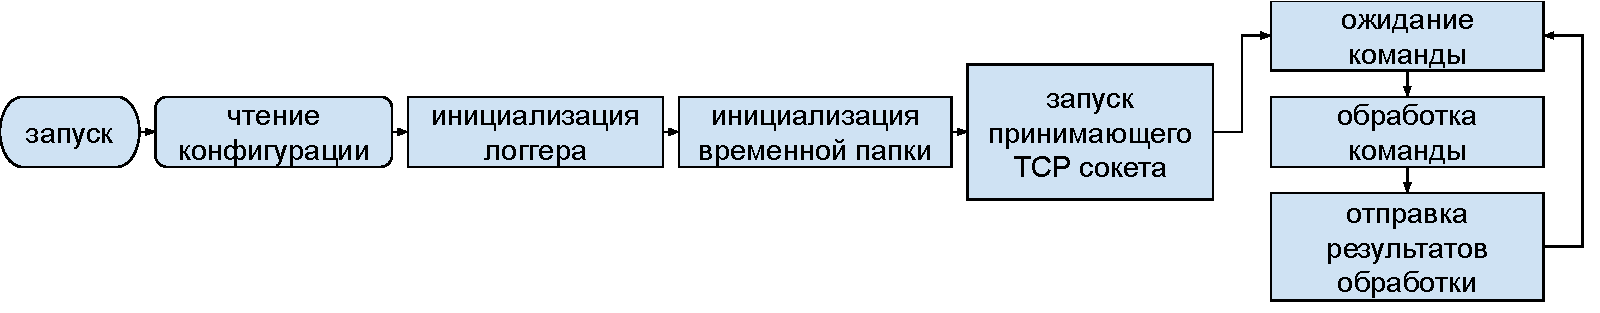
\includegraphics[width = 0.98\textwidth]{img/nu_mass_setup/detector_workflow.pdf}
    \caption{Схема работы сервиса детектора.}
    \label{fig:numass-detector-workflow}
\end{figure}

В целях достижения гибкости настройки адреса всех модулей КАМАК могут быть заданы через конфигурационный файл, который считывается на стадии “чтение конфигурации”. В случае некорректной конфигурации приложение выведет соответствующие предупреждения в консоль. Также, в целях дублирования во избежание потери данных при инициализации сервис создает временную папку, в которую будут записываться последние набранные файлы.

\subsubsection{Взаимодействие с КАМАК}\label{camac-interaction}
Сервис взаимодействует с модулями крейта по средствам API предустановленной в ОС CCPC7 библиотеки взаимодействия с КАМАК.

Основной задачей сервиса детекторного модуля является запуск записи событий на блоке КАМАК MADC и их считывание после набора. Полная последовательность команд КАМАК для набора событий за заданное время выглядит можно описать последовательностью:

\begin{enumerate}
    \item TTL\_NIM, команда 0, 17, 0xFFFF - отключение TTL на MADC
    \item MADC, команда 0, 12, none - отключение набора на MADC
    \item MADC 0, 17, time - запись времени набора в MADC
    \item COUNTER1, команда 0..6, none - обнуление значений с 0 по 6 на первом каунтере
    \item COUNTER2, команда 0..6, none - обнуление значений с 0 по 6 на втором каунтере
    \item MADC, команда 0, 11, none - включение набора на MADC
    \item OV1, команда 0, 16, 0x1F - включение всех выходов на OV1, верхний канал
    \item OV1, команда 0, 16, 0x0F - включение всех выходов на OV1, нижний канал
    \item OV1, команда 0, 25, none - запуск OV1 в импульсном режиме. После этой команды начинается аппаратный набор событий
    \item Цикл опроса MADC - завершается при выставлении флагов завершения или переполнения
    \begin{enumerate}
        \item Ожидание 1 с
        \item MADC, команда 1, 1 - считывание количества набранных событий, \ флагов завершение набора или переполнения буфера
        \end{enumerate}
        \item MADC, команда 0, 12, none - отключение набора на MADC
        \item MADC, команда 1, 1 - считывание полного количества набранных событий
        \item Цикл чтения событий
        
        \begin{enumerate}
        \item MADC, 0, 0, none - считывание младших 2 байт времени события
        \item MADC, 1, 0, none - считывание старших 2 байт времени события
        \item MADC, 2, 0, none - считывание амплитуды и флага корректности события события
    \end{enumerate}
\end{enumerate}

\bigskip

Также предоставляет метод API по инициализации крейта КАМАК, которая последовательно выполняет команды Z и C.

\subsubsection{Инициализация КАМАК}

Перед работой с сервисом необходимо проинициализировать крейт детектора. Для этого необходимо подключиться к серверному сокету сервиса и передать dataforge-envelope пакет с пустой бинарной частью и с следующими полями в корне метаданных:

\begin{lstlisting}[caption={Команда иниализации крейта КАМАК детектора.}, captionpos=b]
{ "command_type" : "init",
  "type" : "command" }
\end{lstlisting}

Здесь type - тип пакета. Для всех команд значение этого поля должно быть “command”; command\_type - тип команды. В данном случае это код команды инициализации - “init”.

При получении команды сервис последовательно выполнить команды крейта Z и C. После выполнения сервис передаст ответ:

\begin{lstlisting}[caption={Сообщение об успешной иниализации сервиса детектора.}, captionpos=b]
{ "type" : "reply",
  "reply_type" : "init",
  "reseted" : "1",
  "status" : "ok" }
\end{lstlisting}

Здесь type - тип ответа. В системе сбора данных Троицк ню-масс для ответов это поле может иметь только значение reply, reply\_type - тип ответа, status - статус команды (практически для всех команд значение равно ok), reseted - флаг перезагрузки сервера (0 - если сервер проинициализирован в первый раз, 1 - в противном случае).

\subsection{Набор событий с детектора}

После инициализации крейта детектора, с помощью сервиса можно начать проводить набор событий, регистрируемых детектором. Для этого на сервис необходимо передать пакет с метаданными:

\begin{lstlisting}[caption={Пример команды на набор событий.}, captionpos=b]
{  "acquisition_time" : "5",
     "command_type" : "acquire_point",
     "type" : "command",
     "split" : "true",
     "external_meta": {
       "HV1_value": "-1", 
       "HV2_value": "-1",
       "acquisition_time": "5",
       "point_index": "0" } }
\end{lstlisting}
Здесь:
\begin{itemize}
    \item acquisition\_time - Время набора в секундах.
    \item split - флаг разделения набора на поднаборы по 5 с. 
    \item external\_meta - Опциональный контейнер для внешних метаданных. Предназначен для сохранения информации о точке, полученной извне (например напряжение на спектрометре при наборе). Поле будет полностью скопировано в такой же тег в ответе.
\end{itemize}

При обработке такой команды сервис выполнит, описанную в параграфе \ref{camac-interaction} последовательность действий для набора событий в течение фиксированного времени. В случае, если в команде указывается флаг разделения набора, описанная последовательность будет выполнена несколько раз для времени 5 с и общим временным покрытием равным заданному времени набора. Производить набор с разделением следует в случае высокой скорости счета и больших желаемых времен набора, т.к. разделение позволяет избежать переполнение памяти MADC при наборе.

В случае набора без разделения сервис выдаст ответ по типу:
\begin{lstlisting}[caption={Сообщение с набранными событиями (набор без разделения).}, captionpos=b]
{   "binary_size": "2345",
     "end_time": "15:56:27.109",
     "external_meta": { "HV1_value": "-1",
                        "HV2_value": "-1",
                        "acquisition_time": "5",
                        "point_index": "0" },
     "format_description": "https://...",
     "programm_revision": "1.59aa102",
     "reply_type": "aquired_point",
     "start_time": "15:56:22.065",
     "status": "ok",
     "time_coeff": 50,
     "total_events": "335",
     "type": "reply" }
\end{lstlisting}
Здесь: binary\_size - размер полученных бинарных данных в байтах, start\_time - приблизительное время начала набора точки, end\_time - Приблизительное время окончания набора точки, time\_coeff - коэффициент преобразования из внутреннего времени в наносекунды, total\_events - количество сосчитанных событий в точке, external\_meta - контейнер для внешних метаданных, format\_description - ссылка на описание формата бинарных данных, programm\_revision - версия программы, с помощью которой набрана точка.

Бинарные данные в ответном пакете будут содержать параметры событий в бинарном формате MADC.
Для набора с разделением ответное сообщение будет немного отличаться:
\begin{lstlisting}[caption={Сообщение с набранными событиями (набор с разделением).}, captionpos=b]
{  "acquisition_time": 10,
   "binary_size": "455300",
   "end_time": [
     "2017-11-22T11:15:09", 
     "2017-11-22T11:15:15"],
   "events": [ 32359, 32483 ],
    "external_meta": { "HV1_value": "-1",
                        "HV2_value": "-1",
                        "acquisition_time": "10",
                        "point_index": "0" },
    "format_description": "https://...",
    "programm_revision": "1.1.1-70-gd158942",
    "reply_type": "aquired_point",
    "split": true,
    "start_time": [ 
      "2017-11-22T11:15:04", 
      "2017-11-22T11:15:09" ],
    "status": "ok",
    "time_coeff": 50,
    "total_events": "64842",
    "type": "reply" }
\end{lstlisting}
Из различий здесь start\_time и end\_time теперь имеют векторное значение соответствующее временам набора 5 секундных блоков и добавлено поле events соответствующее количеству событий в каждом блоке. Бинарная часть имеет такой же формат, что и в ответе на набор без разделения. По количеству событий в каждом из блоков можно восстановить отступы в бинарных данных.

\subsection{Модуль стойки высокого напряжения}
На рисунке \ref{fig:numass-hv-workflow} изображена схема работы сервиса.
\begin{figure}
  \centering
  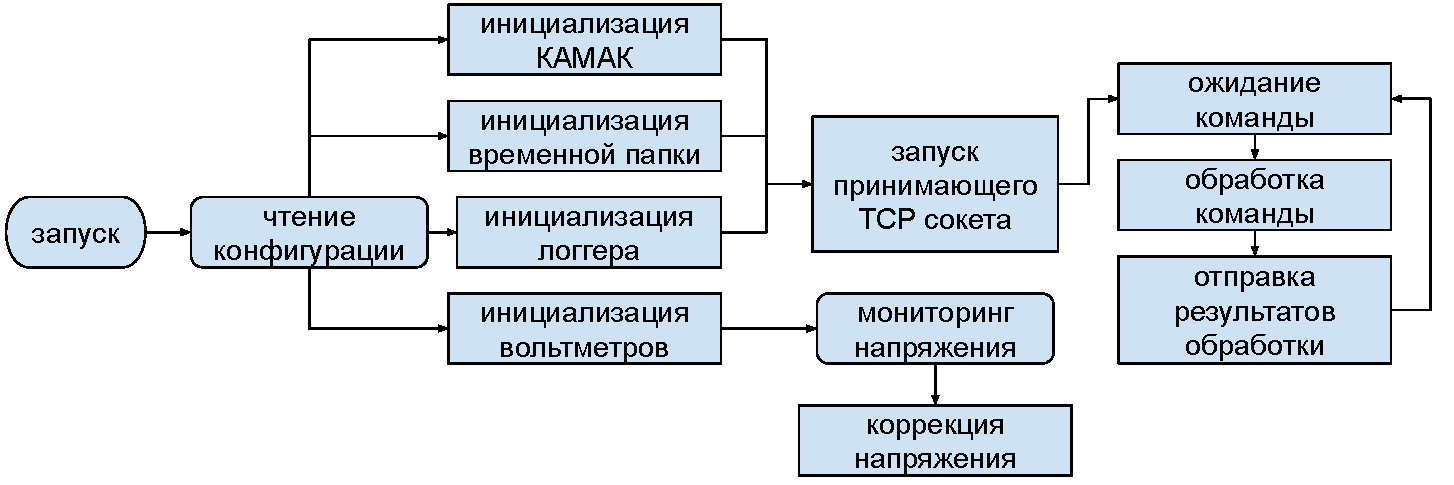
\includegraphics[width = 0.98\textwidth]{img/nu_mass_setup/hv_workflow.pdf}
    \caption{Схема работы сервиса высоковольтной стойки.}
    \label{fig:numass-hv-workflow}
\end{figure}
Аппаратно, сервис соединяется с блоками питания с помощью:
\begin{enumerate}
    \item ЦАП, управляемого через КАМАК и порта RS-232 самого БП для основного блока питания. Необходимость использования КАМАК для взаимодействия с ЦАП отсутвием другой аппаратной части, обеспечивающей задание значений необходимой битности. По сути КАМАК в этом сервисе используется только для программного управления ЦАП.
    \item Порта RS-232 для блока питания смещения.
\end{enumerate}
Порты RS-232 подключаются к CCPC7 через по USB через конвертеры. Аналогично к CCPC7 через RS-232 подключаются вольтметры.

Сервис может работать в 2-х режимах выставления напряжения:

\begin{enumerate}
    \item Выставление напряжения через 2 блока питания. В таком режиме сначала выставляется базовое напряжение и затем с помощью первого блока питания через ЦАП и com порт БП. Затем от базового напряжения вычитается напряжение на втором блоке питания. Т.к. второй блок питания может изменять напряжения в пределах 1 кВ, такой режим подходит для проведения прецизионных измерений в небольшом диапазоне энергий.
    \item Выставление напряжения с помощью одного блока питания. Этот режим аналогичен предыдущему за исключением отсутствия второго шага и подходит для набора данных в широком диапазоне энергий.
\end{enumerate}
Необходимый режим работы сервиса можно задать через конфигурационный файл.

При запуске приложения, после чтения конфигурации сервис также как и в модуле детектора проводит инициализацию логгера и временной папки. Далее автоматически проводится инициализация КАМАК, при которой на вход ЦАП выставляется значение 0. Инициализация здесь происходит автоматически для минимизации рисков нежелательного выставления напряжения на блок питания, т.к. начальные значения при старте КАМАК отличны от нуля. Параллельно происходит инициализация вольтметров. В режиме работы с одним блоком питания инициализируется только один вольтметр - второй может быть использован вручную для сторонних измерений; в режиме с двумя БП- инициализируются оба вольтметра. После успешной инициализации вольтметров запускается отдельный программный поток, осуществляющий мониторинг и коррекцию выставленного напряжения.

\subsubsection{Коррекция напряжения}

В процессе эксплуатации системы выяснилось, что выставляемое через вольтметры напряжение в действительности задается с плавающей ошибкой порядка 7 В. Для устранения этой ошибки в работу сервиса был встроен алгоритм коррекции. Описать его можно следующей последовательностью.

\begin{enumerate}
\item При установке напряжения через ЦАП устанавливается основная часть напряжения - 100 В. Оставшиеся 100 В устанавливаются через RS-232 и обеспечивают запас для коррекции. 
\item При измерении напряжений на вольтметре сервис записывает во внутренний буфер последние 3 измерения. 
\item При каждом новом измерении напряжения на вольтметре, если разница между текущим и предыдущим измерениями оказывается меньше заданного порога (т.е. напряжение стабилизировано) и при этом измеренное напряжение отличается от желаемого - к 100 В, устанавливаемым через RS-232 добавляется или вычитается значение, равное разнице между измеренным и желаемым напряжениями.
\end{enumerate}
Описанный метод коррекции напряжения позволяет добиться стабильной точности при выставлении порядка десятых долей Вольта.

\subsubsection{Инициализация вольтметров}

Инициализация и управление вольтметрами происходит через RS-232 порт и описывается последовательностью действий:

\begin{enumerate}
\item Перевод вольтметра в режим программного контроля.
\item Выставление необходимой точности.
\item Выставление мода медленного изменения напряжения.
\item Выставление сопротивления 10 ГОм.
\item Выставление конфигурации для медленных измерений.
\end{enumerate}
После сервис в цикле проводит последовательное чтение напряжения. Считанные данные отправляются клиенту, если он подключен, автоматически без запроса на измерение.

\subsubsection{Выставление напряжения}

После подключения, через сервис можно задать напряжение на блоке питания. Для этого по сокету необходимо отправить пакет, содержащий метаданные:

\begin{lstlisting}[caption={Команда на выставление напряжения спектрометра.}, captionpos=b]
{  "block": "1",
   "command_type" : "set_voltage",
   "type" : "command",
   "voltage": "16.1818" }
\end{lstlisting}
Здесь block - номер блока питания (1 - основной, 2 - блок смещения), voltage - желаемое напряжение в Вольтах.

После получения команды, сервис выставит через ЦАП и RS-232 необходимое напряжение и начнет проводить непрерывную коррекцию к заданному уровню. После выставления по каналу сокета будет передан ответ:

\begin{lstlisting}[caption={Сообщение об успешном выставлении напряжения на спектрометра.}, captionpos=b]
{  "type": "answer",
   "block" : "1",
   "answer_type" : "set_voltage",
   "status": "ok" }
\end{lstlisting}

Сервис также имеет возможность задания напряжения с ожиданием его выставления. Запрос такой команды немного отличается:

\begin{lstlisting}[caption={Команда на выставление напряжения спектрометра с последующей проверкой.}, captionpos=b]
 {  "block": "1",
    "command_type" : "set_voltage_and_check",
    "type" : "command",
    "voltage": "16.1818",
    "max_error": 5,
    "timeout" : 20 }
\end{lstlisting}
Здесь max\_error - допустимая ошибка в Вольтах, timeout - максимальное время ожидания в секундах.

Ответ на команду придет только после того как измерения вольтметра будут совпадать с желаемым значениям в пределах погрешности.

\subsection{Управляющий модуль}

На клиентском компьютере, с которого осуществляется управление набором данных должен быть установлен управляющий программный комплекс системы сбора данных. Он состоит из GUI управления и GUI визуализации данных. Т.к. используемая при разработке библиотека QCustomPlot имеет утечку памяти, программу управления было решено разделить на 2 подпрограммы во избежания вылетов во время набора.

Управляющая программа позволяет:

\begin{enumerate}
    \item Подключаться к сервису детектора и проводить набор событий за \ фиксированное время вручную.
    \item Подключаться к сервису высоковольтной стойки задавать и измерять напряжение на блоках питания вручную.
    \item Проводить серии наборов событий, регистрируемых детектором по сценарию. Шагами сценария могут быть:
    \begin{enumerate}
        \item Выставление напряжения на блоке питания спектрометра,
        \item Выставление напряжения на блоке питания спектрометра с последующей проверкой показаний вольтметра,
        \item Запись событий, регистрируемых детектором за фиксированное количество времени,
        \item Второй и третий подпункты одновременно (набор точки).
    \end{enumerate}
    \item Для сценариев, содержащих только команды по набору точек возможен набор обратным проходом.
    \item Сценарий может быть выполнен несколько раз, в т.ч. с чередованием проходов.
\end{enumerate}

\chapter{Расширения системы сбора}
За время эксплуатации новой системы сбора данных периодически появлялась необходимость в изменении ее конфигурации, добавлению и замене элементов. Благодаря выбранным в начале разработки паттернам проектирования, все необходимые модификации проводились относительно просто. В этой главе будут описаны два основных расширения системы, на примере которых можно посмотреть архитектуру в действии и оценить ее эффективность.

\section{Интеграция Лан10-12PCI}\label{lan10-integration}
Переход установки <<Троицк ню-масс>> на поиск стерильных нейтрино требует повышения скорости счета в системе регистрации событий. Для этого было сделано расширение системы, которое добавило новый модуль обработки сигнала детектора, основанный на АЦП Лан10-12PCI.

В целях тестирования, оба модуля были подключены к сигналу детектора и настроены на синхронный набор данных.
На время отладки нового модуля Лан10-12PCI, дублирующие данные MADC использовались для контроля качества и оценки корректности обработки. Схема подключения представлена на рисунке \ref{fig:numass-lan10-integration}.
\begin{figure}
  \centering
  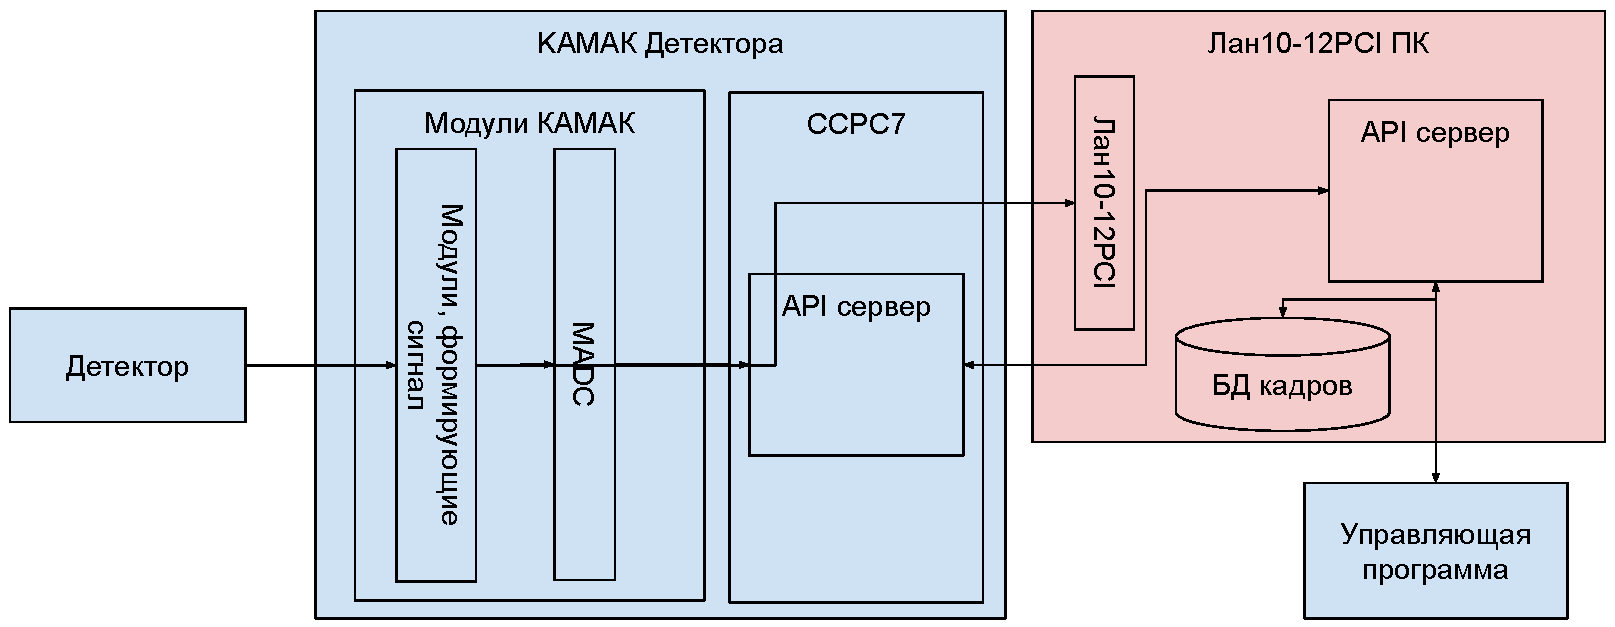
\includegraphics[width = 0.98\textwidth]{img/nu_mass_setup/lan10-integration.pdf}
    \caption{Подключение платы Лан10-12PCI. Розовым цветом обозначены новые модули системы.}
    \label{fig:numass-lan10-integration}
\end{figure}

Поступающий с детектора сигнал после формирования модулями КАМАК детектора делится и теперь кроме входа в MADC также входит в плату АЦП Лан10-12PCI, которая установлена в отдельном компьютере. На этом же компьютере запущен API сервис протокол сообщений которого полностью совпадает с протоколом API сервера, установленного на CCPC7. Для набора с обоих модулей управляющей нужно переподключиться к новому API серверу, если же не делать этого - то при наборе будет работать только старая система.

Новый API сервер работает как <<сниффер>> между стандартным детекторным блоком и управляющей программой.
При получении команды от управляющей программы, сервер передает ее в CCPC7 без изменений. Ответы на команды, приходящие от КАМАК также прозрачно транслируются обратно в управляющую программу. В случае, если через сервер проходит команда на набор событий - помимо передачи команды на CCPC7 программа также запустит набор кадров через плату Лан10-12PCI с таким же временем набора. После завершения набора обеими системами на управляющую программу программу будет передан ответное сообщение аналогичное ответу на набор точки API сервера CCPC7. Т.к. набираемые новой системой кадры получаются значительно больше данных MADC в целях экономии передаваемого трафика и минимизации проблем, создаваемых высокими нагрузками на сеть, данные  Лан10-12PCI после набора сохраняются локально на жесткий диск ПК. Синхронизация с общей БД проводится один раз после завершения сеанса сбора данных.

Архитектура системы сбора разделяет работу по самостоятельным компонентам и инкапсулирует всю специфичную обработку внутри, выводя во вне только программно-независимый API. Благодаря этому описанное расширение системы потребовало создать всего один новый сервис. Существующие компоненты при этом остались без  каких-либо изменений. Для работы в дублирующем режиме в управляющей программе необходимо только изменить ip адрес и порт сервиса детектора. Также просто можно отключить новую систему, что может быть полезно в случае появления неполадок в ее работе.

\subsection{Python-df-tcp}
Для ускорения разработки сервиса, было решено реализовать программу на языке Python. Исходники можно найти в репозитории \cite{counter-redirecter}. Сам сервер создан на базе подпроекта python-df-tcp\cite{python-df-tcp}, реализующего виртуальные классы сервисов использующих в качестве протокола обмена сообщениями формат dataforge-envelope. Проект python-df-tcp использует библиотеку Python 3, asyncio и предоставляет базовые классы для сервера и клиента. В теле базового класса реализован функционал по приему, склейке и отправки сообщений обратно по TCP/IP подключению.

Пример реализации эхо-сервера на базе df-tcp будет выглядеть:
\begin{lstlisting}[language=Python,style=protobuf]
import asyncio

from dftcp import DataforgeEnvelopeProtocol


class EchoServerProtocol(DataforgeEnvelopeProtocol):
    """Echo server protocol."""

    def process_message(self, message):
        """Send original message back to receiver."""
            print("receive {}, {}".format(
                message['meta'], message["data"]))
            self.send_message(
                message['meta'], message["data"], 0)


if __name__ == "__main__":
    loop = asyncio.get_event_loop()
    coro = loop.create_server(EchoServerProtocol, "0.0.0.0", 5555)
    server = loop.run_until_complete(coro)

    print('Serving on {}'.format(server.sockets[0].getsockname()))

    try:
            loop.run_forever()
    except KeyboardInterrupt:
            print("Programm stoped by user input")

    server.close()
    loop.run_until_complete(server.wait_closed())
\end{lstlisting}

Как видно по приведенному скрипту весь процесс обработки сообщений упакован в переопределенный метод process\_message, который, с помощью метода send\_message базового класса DataforgeEnvelopeProtocol отправляет приходящее сообщение обратно отправителю. В условии \_\_main\_\_ приведен код для стандартно запуска сервера на asyncio.

Пример реализации скрипта эхо-клиента на базе df-tcp выглядит:
\begin{lstlisting}[language=Python,style=protobuf]
import asyncio

from dftcp import DataforgeEnvelopeEchoClient as DFClient


def callback(message, client_obj):
    """Print received message."""
    print("receive {}, {}".format(message["meta"], message["data"]))
    client_obj.transport.close()


if __name__ == "__main__":
    loop = asyncio.get_event_loop()
    coro = loop.create_connection(lambda: DFClient(
        loop=loop, meta=dict(field="value"), data=b"binary",
        callback=callback, timeout_sec=30), "localhost", 5555)
    loop.run_until_complete(coro)
    loop.run_forever()
\end{lstlisting}

Здесь задание передаваемых данных и параметров подключения устанавливается методом create\_connection в условии \_\_main\_\_. Функция callback определяет обработку ответа от сервера. В примере это вывод содержимого пакета в консоль и последующее закрывание канала сокета.

Описанный примером функционал позволяет создавать на базе модуля df-tcp сервисы, использующие протокол dataforge-envelope, в частности сервер осуществляющий прозрачную передачу пакетов на API сервис КАМАК детектора, который будет описан далее.

\subsection{Набор кадров с помощью Лан10-12PCI}
Для работы с платой Лан10-12PCI ранее на C++ было написано консольное приложение lan10-12pci\_base, реализующее cli для работы с платой. Следуя DRY принципу, было решено использовать lan10-12pci\_base без изменений в качестве средства взаимодействия с платой. Т.к. формат управления приложением отличается от используемого в системе сбора данных Троицк ню-масс, для работы был написан конвертер, преобразующий выходные данные в формат dataforge-envelope. 

Схема работы сервиса Лан10-12PCI в режиме набора событий с детектора изображена на рисунке \ref{fig:numass-lan10-workflow}.

\begin{figure}
  \centering
  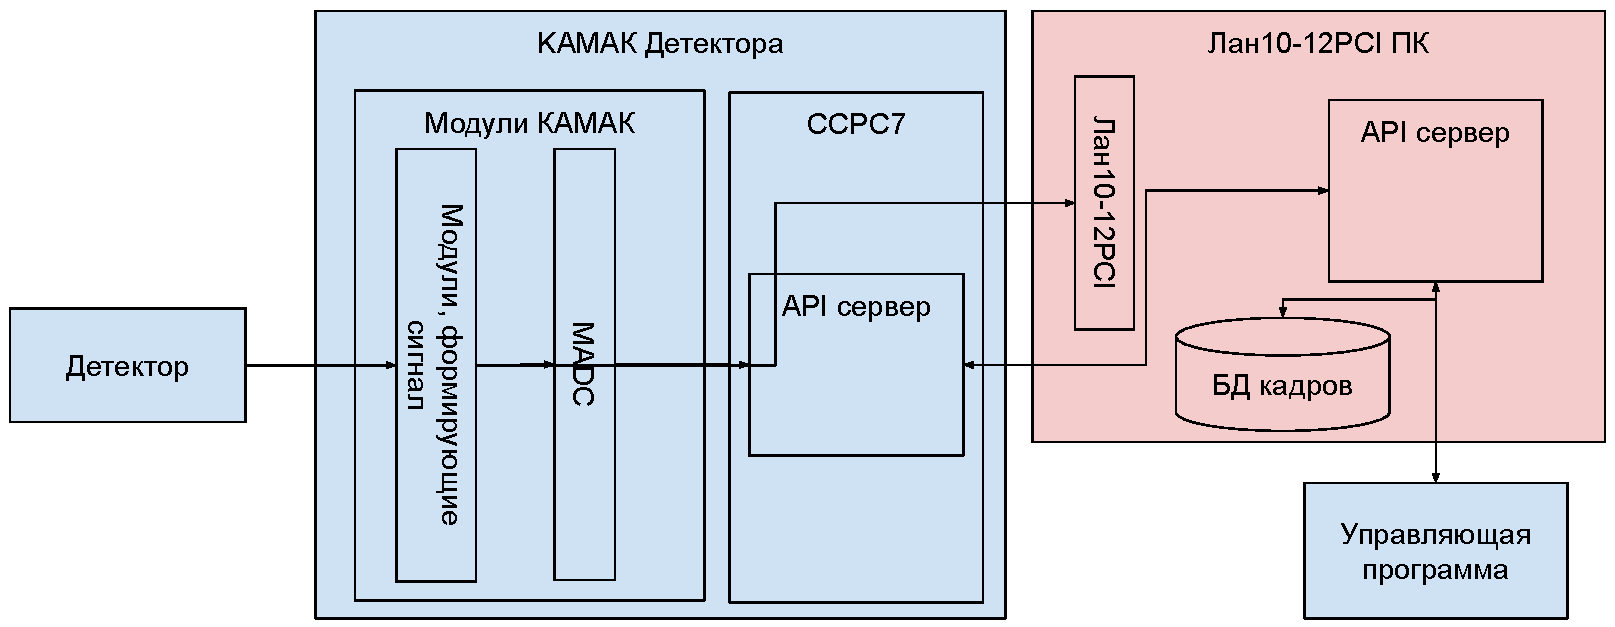
\includegraphics[width = 0.98\textwidth]{img/nu_mass_setup/lan10-integration.pdf}
    \caption{Подключение платы Лан10-12PCI. Розовым цветом обозначены новые модули системы.}
    \label{fig:numass-lan10-workflow}
\end{figure}
При получении команды на набор, пакет содержащий ее сразу транслируется в сервис КАМАК детектора. Одновременно с этим во временной директории Лан10-12PCI ПК создается конфигурационный файл имеющий совместимый с lan10-12pci\_base формат и содержащий аналогичные с КАМАК параметры набора. После создания конфигурации сервер запускает программу lan10-12pci\_base в тихом режиме и передает ей созданный файл. К завершению создаваемого процесса привязан колбэк, который запускает предварительную обработку в виде алгоритма zero-suppression и последующее конвертацию полученных кадров событий в пакет dataforge-envelope и сохранение на диск. После сохранения программа ожидает ответа от сервиса MADC. При получении ответа MADC происходит транслирование его в управляющую программу. Т.к. для создание конфигурационного файла для программы ~lan10-12pci\_base происходит мгновенно, обе системы имеют практически полное пересечение наборов по времени. Конвертация выходных данных программы lan10-12pci\_base тоже происходит практически сразу и не вносит дополнительного ожидания по сравнению с обычным набором. Описанный алгоритм дожидается окончания набора обеих систем, что исключает наложение команд и создание очереди набора, которая может привести к несооветвию результатов работы систем при обработке одной и той же команды.

Файлы, набираемые сервисом Лан10-12PCI отличаются по формату от файлов MADC:
\begin{lstlisting}[caption={Сообщение с набранными платой Лан10-12PCI событиями.}, captionpos=b]
{  "bin_offset": 0,
   "bin_size": 83483520,
   "external_meta": {
        // ...
    "process_params": { "area_l": 100,
                            "area_r": 200,
                            "threshold": 750 },
    "params": { /* ...  */ },
"compression": "zlib" } }
\end{lstlisting}

Отличие в отсутвии в корне метаданных полей, относящиеся к событиям, такие как: полное количество зарегистрированных событий, коэффициенты перевода времени. В корне остаются только 2 поля: bin\_offset - отсуп в байтах в бинарной части пакета, bin\_size - размер бинарной части пакета в байтах. Также в словарь external\_meta записываются дополнительные поля: process\_params - параметры обработки zero-suppression и params - конфигурация Лан10-12PCI, используемая при наборе и сконвертированная из конфигурационного файла в JSON.

\subsection{Настройка Лан10-12PCI ПК}
Т.к. в течение экспериментального сеанса данные, набранные платой Лан10-12PCI находятся только в одном месте - на Лан10-12PCI ПК - для просмотра и анализа данных в реальном времени была создана программа, реализующая web-интерфейс с возможностью просмотра набираемых файлов. Дизайн интерфейса подобен дизайну DataVisualizer. Бэкенд сервера написан на Python с использованием фреймворка Flask. Бэкенд реализует методы API по выводу дерева файлов в локальной БД, считыванию метаданных файла набора, построение в реальном времени гистограммы для файла с последующим кэшированием результатов. При генерации гистограммы для преобразования кадров в события используется простой поиск максимума в кадре, что достаточно для визуального представления данных и оптимально по скорости обработки. Фронтенд web интерфейса написан на JavaScript с использованием TypeScript в качестве метаязыка. Для визуализации графических данных используется библиотека Plotly.js. Для остальных элементов интерфейса использовалась библиотека Bootstrap. Интерактивность страницы обеспечивается библиотекой JQuery. Исходный код сервера web интерфейса выложен в репозиторий \cite{lan10-viewer}.

На Лан10-12PCI ПК в качестве ОС установлена Ubuntu 16.04. Для удобства использования комплекса сервис Лан10-12PCI и web-интерфейс запускаются автоматически при включении компьютера. Автозапуск реализован с помощью встроенного в Ubuntu сервиса systemd. Для инкапсулирования Python зависимостей в каждом проекте использовался модуль Pipenv. Чтобы обеспечить совместимость генерируемой Pipenv среды и systemd, в конфигурацию сервиса в поле исполняемой команды в качестве интерпретатора Python задается путь к ссылке python, находящейся непосредственно в создаваемой Pipenv папке среды.

В ходе эксплуатации Лан10-12PCI на Linux, выяснилось, что поставляемые компанией Руднев-Шиляев драйвера для Linux ведут себя нестабильно при обновлениях системы - часто при перезапуске Лан10-12PCI ПК и последующем запуске набора оказывалось, что драйвер не видит установленной в компьютер платы АЦП. Скорее всего причиной этой проблемы является несовместимость ранее установленной версии драйвера и новой версии ядра Linux, устанавливаемого при обновлении пакетов. Найденное решение проблемы заключается в полной переустановке всех драйверов RudShel и последующем перезапуске компьютера.

\subsection{Тестирование набора кадров с помощью платы Лан10-12PCI}
Переход на набор непрерывных кадров помимо модернизации аппаратной части системы набора событий требует также проведения тестирования и валидации качества набора новой системы. Для этого на всех сеансах с участием новой платы Лан10-12PCI, набор проводился одновременно двумя системами: с помощью MADC и с помощью непосредственно Лан10-12PCI. Помимо этого, вместе с сигналом детектора к обоим системам был подключен также тестовый генератор, обеспечивающий стабильные периодические импульсы с постоянными частотой равной 50 Гц и амплитудой, величина которой заведомо выше амплитуд набираемых с детектора событий. Эти два условия позволяют проводить сравнение набираемых данных и обеспечивают возможность качественной оценки корректности работы новой системы набора. При сравнении, для выделения параметров событий из набираемых платой Лан10-12PCI кадров был использован второй метод, описанный в главе “Обработка кадров непрерывного сигнала”. В описанном далее сравнении будут рассматриваться данные, набранные на сеансе 2017\_05.

\subsubsection{Поиск функции перехода между MADC и Лан10-12PCI}
Для сравнения данных двух систем прежде всего необходимо перевести их в одни единицы измерения. Данные платы Лан10-12PCI имеют особенность - из-за записи реальных 12-битных амплитуд в 16-битные значения, все набранные значения имеют дискретное распределение амплитуд кратное 16. Это накладывает сильные ограничения на возможность преобразований - т.к. при гистограммировании необработанных данных во избежания появления артефактов необходимо выбирать биннинг также кратный 16; если же с данными проводились преобразования, то для подбора правильного биннинга (не создающего артефактов) необходимо сначала определить исходный, кратный 16 биннинг и затем применить к нему то же преобразование что и к данным. В реальной обработке это довольно накладная процедура, т.к. требует дополнительных расчетов. Зная эту особенность и учитывая тот факт, что на данных MADC такого не происходит, было решено использовать единицы измерения Лан10-12PCI как основные и искать функцию перехода от единиц измерения MADC к  Лан10-12PCI, а не наоборот. Т.о. при преобразованиях данные Лан10-12PCI не будут изменяться, что облегчит дальнейший подбор правильного биннинга.

Посмотрим на данные: на графиках \ref{fig:testing-shapes} изображены типичные спектры для мониторных точек набираемые системами MADC и Лан10-12PCI.

\begin{figure}
  \centering
  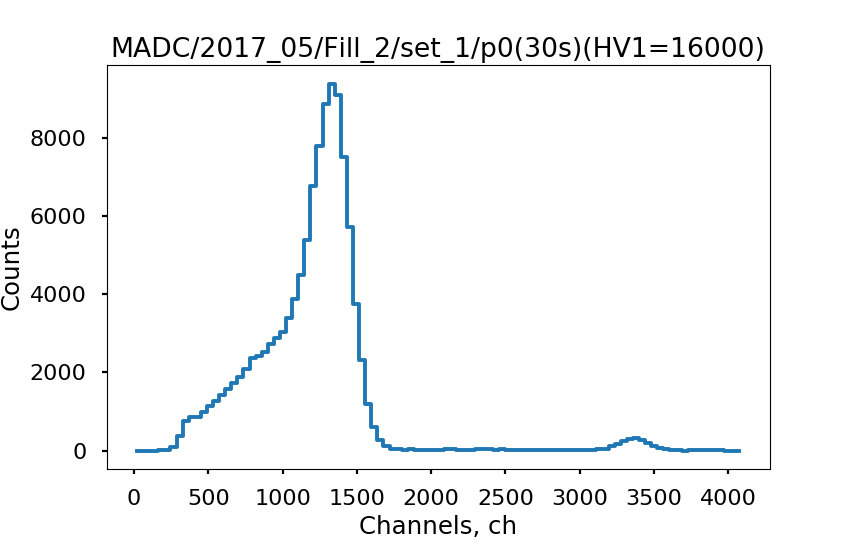
\includegraphics[width = 0.45\textwidth]{img/testing/madc_point_shape.png}
  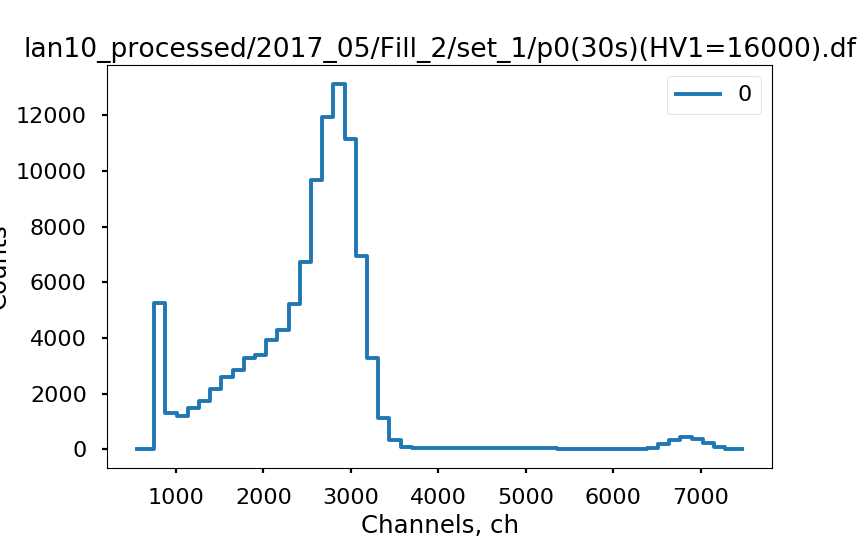
\includegraphics[width = 0.44\textwidth]{img/testing/lan_point_shape.png}
    \caption{Формы спектра одинаковой точки для модуля MADC (слева) и Лан10-12PCI (справа)}
    \label{fig:testing-shapes}
\end{figure}

Как из них видно набранные спектры для обеих систем визуально совпадают совпадают. Справа от амплитудных спектров реальных событий, поступающих с детектора, можно увидеть небольшой пик - это гистограмма созданных тестовым генератором событий событий. Также можно заметить, что форма амплитудных спектров генератора напоминает функцию Гаусса, а положение максимума которой приходится примерно на 3400 канал для данных MADC и примерно 6800 канал для платы Лан10-12PCI. Предварительно можно сказать, что масштабы шкал будут различаться примерно в два раза. Однако помимо отличий в масштабе единиц изменения данные могут иметь также отличающиеся нули координат. Учитывая вид данных: их визуальное сходство, явную линейность шкал и возможное потенциальное отличие нулей для обеих систем в качестве функции перехода было решено взять полином первой степени со свободным членом. Т.к. в набранных системами файлах самым стабильным и известным объектом является амплитудный спектр событий, создаваемых тестовым генератором, коэффициенты выбранной функции перехода будут рассчитываться именно по нему. Расчет обоих коэффициентов возможен в силу наличия у спектра аналитической функции обладающей максимумом и шириной.

\subsubsection{Алгоритм подбора коэффициентов}

Алгоритм поиска коэффициентов между системами можно описать следующей последовательностью операций:
\begin{enumerate}
    \item Объединение данных сета. Отдельный файл, время набора которого составляет 30 с) вследствие малой скорости счета тестового генератора в 50 Гц содержит примерно 1.5к событий, чего недостаточно для точного расчета коэффициентов. Сет в свою очередь содержит 107 точек которые суммарно содержат порядка 160к событий генератора - этого количества становиться уже достаточно. Объединение генераторных событий из всех точек сета позволяет построить амплитудный спектр с достаточной точностью.
    \item Гистограммирование событий объединенных файлов всего сета. 
    \item Вырезание из полученных гистограмм для MADC и Лан10-12PCI амплитудных спектров создаваемых генератором событий, т.к. из всего спектра для расчета коэффициентов мы будем пользоваться только ими. При вырезании для обоих спектров в целях сохранения правильности отступов используются абсолютные значения амплитуд относительно нуля.
    \item Фитирование обоих пиков функцией Гаусса. Получение значений положений максимума и ширины гауссиана для данных MADC и Лан10-12PCI. Переход от численных спектров к аналитическим функциям с подобранными фитированием коэффициентами обеспечивает большую стабильность алгоритма поиска функции перехода между двумя системами.
    \item Вычисление коэффициентов перехода между двумя полученными гауссианами. Полученные коэффициенты будут являться также и коэффициентами перехода между спектрами реальных событий детектора.
\end{enumerate}

Как было сказано ранее, в качестве функции перехода была выбрана линейная функция со свободным членом. Формула перехода данных MADC к Лан10-12PCI может быть выражена формулой $ x_m= a x_l + b $, где $ x_l $- амплитуда набранного с помощью  Лан10-12PCI события, $ x_m $- амплитуда события MADC, $ a $ - коэффициент масштабирования между шкалами MADC и Лан10-12PCI, $ b $ - отступ нуля Лан10-12PCI от нуля MADC в единицах измерения MADC.

Для расчета отступа нуля a используется формула $ a= \frac{\delta_l}{\delta_m} $, где $ \delta_l, \delta_m $ - среднеквадратичные отклонения построенных фитированием функций Гаусса для Лан10-12PCI и MADC соответственно. Коэффициент масштабирования $ b $ вычисляется по формуле $ b= \mu_l - \mu_m a $,  где $ \mu_l, \mu_m $ - математические ожидания построенных гауссианов Лан10-12PCI и MADC соответственно, $ a $ - рассчитанная ранее разница между отступами.

\subsubsection{Подбор коэффициентов}
При вычислении коэффициентов функции перехода, на этапе гистограммирования для данных MADC использовался размер бина равный 80 каналам и размер бина равный 32  - для платы Лан10-12PCI. На графике \ref{fig:testing-coeff-matching} показан пример амплитудных спектров генераторных событий двух систем, наложенных друг на друга с использованием описанной выше формулы перехода.

\begin{figure}
  \centering
  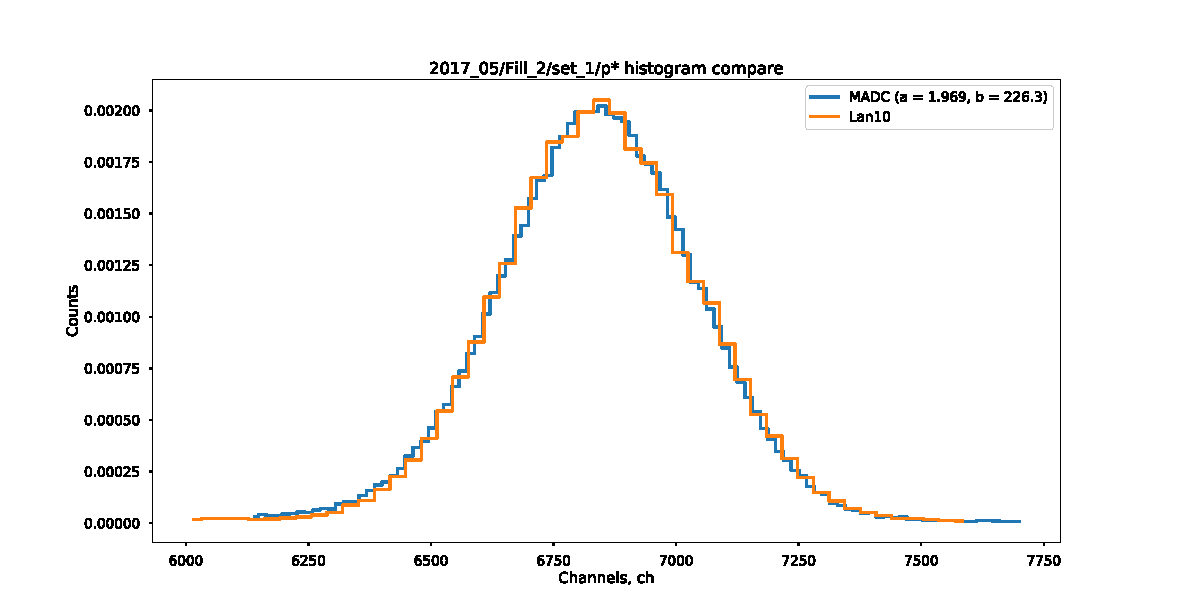
\includegraphics[width = 0.7\textwidth]{img/testing/coeff_matching.pdf}
    \caption{Поиск коэффициентов перехода по генераторным пикам.}
    \label{fig:testing-coeff-matching}
\end{figure}

Для обеспечения соответствия между разными размерами бинов, на этапе поиска коэффициентов фитированием использовались нормализованные на единицу амплитудные спектры. Как видно из графика форма спектров действительно может быть описана функцией Гаусса, а подобранная функция перехода правильно отображает один спектр на другой. В данном примере единицы измерений различаются в 1.969 раза, а разница между нулями систем составляет примерно 226 каналов MADC.

Расчет общих коэффициентов перехода между двумя системами предполагалось получить усреднением коэффициентов по всем физическим сетам сеанса, имеющим генераторные события. Однако в процессе нахождения коэффициентов для сетов выяснилось что их значения существенно отличаются друг от друга. С целью выяснения природы различия значений была построена временная зависимость коэффициентов. 

\begin{figure}
  \centering
  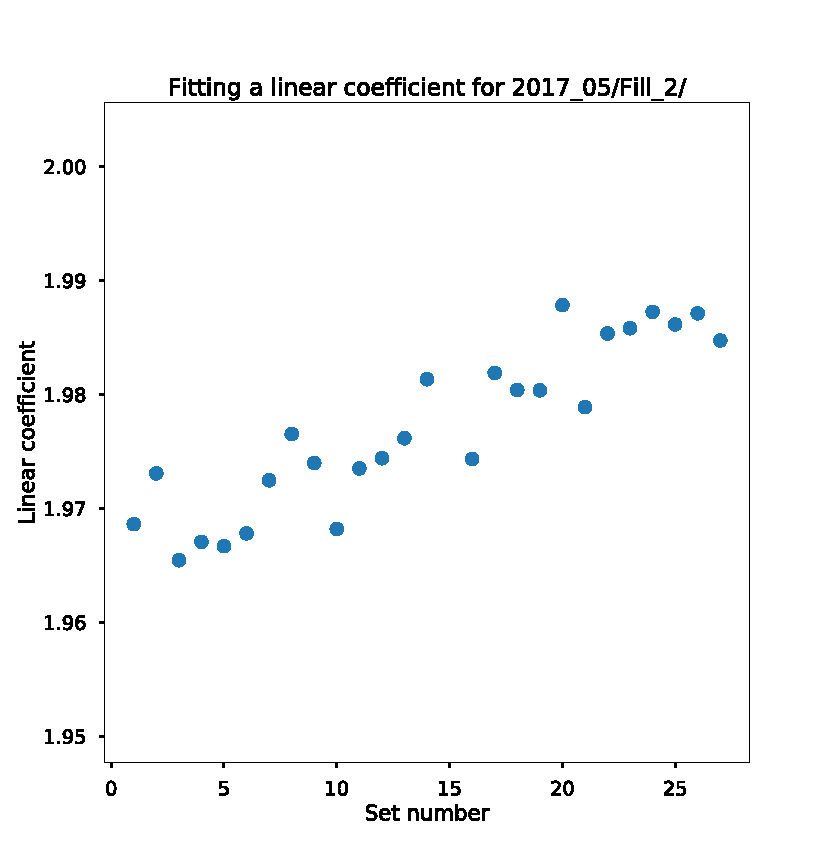
\includegraphics[width = 0.45\textwidth]{img/testing/linear_coeff_dynamic.pdf}
  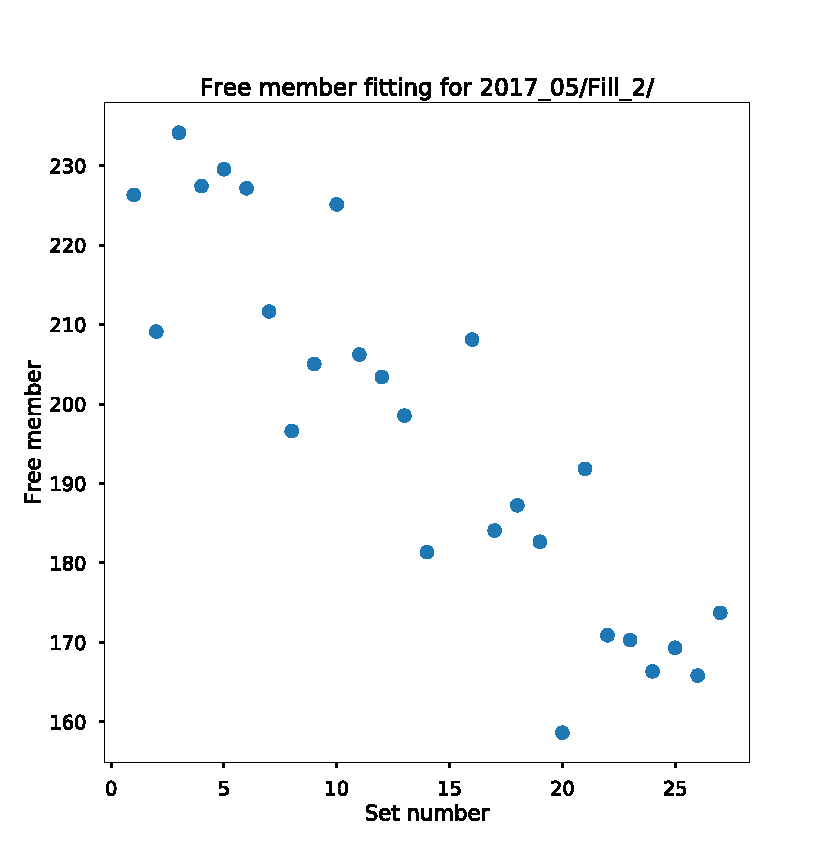
\includegraphics[width = 0.44\textwidth]{img/testing/free_coeff_dynamic.pdf}
    \caption{Изменение коэффициентов перехода между шкалами MADC и Лан10-12PCI.}
    \label{fig:testing-coeff-dynamic}
\end{figure}

Как видно из графиков на рисунке \ref{fig:testing-coeff-dynamic} значения коэффициентов изменяются не случайным образом: на протяжении набора группы Fill\_2 сеанса 2017\_05 коэффициент перехода между шкалами MADC и Лан10-12PCI линейно увеличивался со значения 1.96 до примерно 1.99, а разница между положениями нуля линейно сократилась примерно на 60 каналов MADC: с 230 до 170.

Обнаруженное поведение коэффициентов масштабирования в силу неслучайности отклонений не позволяет получить общие коэффициенты для функции перехода между данными MADC и Лан10-12PCI - для обеспечения точного соответствия необходимо рассчитывать коэффициенты по амплитудным спектрам генераторных точек для каждого сета отдельно. Динамика изменений коэффициентов может свидетельствовать о нестабильности электроники: либо системы набора MADC, либо платы Лан10-12PCI. Причина линейного изменения требует дальнейшего анализа и тестирования работы обоих систем. Однако в целом по полученным результатам можно утверждать что новая система сбора данных, основанная на наборе кадров непрерывного сигнала с помощью платы Лан10-12PCI и дальнейшей обработки программными способами работает стабильно, а получаемые ей спектры с точностью до описанной погрешности совпадают со спектрами старой системы.

\section{Интеграция Dante}

В рамках коллаборации Tristan, на установке Троицк ню-масс был проведен экспериментальный сеанс, на котором было проведено тестирование и отладка прототипа детектора производства лаборатории Макса Планка, Мюнхен\cite{1801.08182}. К финальной версии детектора, которая будет использоваться на установке KATRIN предъявляются следующие требования:

\begin{itemize}
    \item Высокая разрешающая способность и возможность задания низкого порога срабатывания (1 кэВ). Требование обусловлено особенностями измерений - свидетельства существования стерильного нейтрино в набираемых данных будут выражаться в слабом отклонении спектра набираемых амплитуд - чтобы достоверно различать такое отклонение требуется разрешающая способность не менее 300 эВ полной ширины на уровне половины амплитуды при наборе энергий 20 кэВ
    \item Способность обработки высокой скорости счета. Для достоверной проверки гипотезы существования стерильных нейтрино требуется данные имеющие статистическую значимость порядка 10-6. С учетом суммарного планируемого времени набора на установке Katrin, составляющего 3 года, для достижения желаемой точности требуется проводить набор событий на скорости счета порядка 10-8. При максимальных допустимых скоростях счета для современных детектор порядка 105 событий/с требуется создать сегментированный детектор, состоящий из 1000 ячеек, каждая из которых будет набирать события на скорости 105 событий/с.
    \item Большая площадь детектора. Для избавления от эффектов перераспределения заряда между ячейками диаметр пикселя детектора должен быть не менее 2 мм. В то же время для сохранения высокой разрешающей способности, необходимо добиться низкой емкости пикселя детектора
\end{itemize}
С учетом приведенных требований, коллаборацией TRISTAN был создан прототип детектора, представляющий собой дрейфовый кремниевый детектор, сегментированный на 7 гексагональных пикселей. На рисунке \ref{fig:dante-view} представлен внешний вид Dante.

\begin{figure}
  \centering
  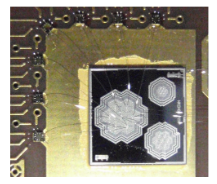
\includegraphics[width = 0.45\textwidth]{img/dante/detector.png}
  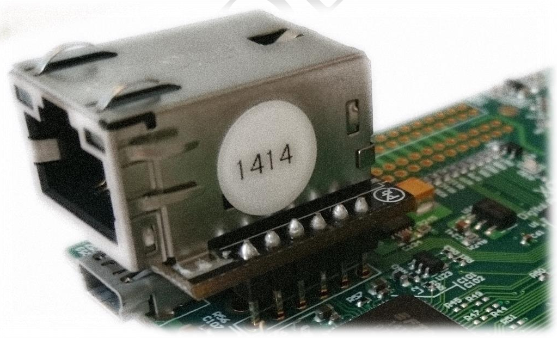
\includegraphics[width = 0.44\textwidth]{img/dante/board.png}
    \caption{Прототип детектора: чувствительная область (слева) и плата Dante (справа).}
    \label{fig:dante-view}
\end{figure}

На установке Троицк ню-масс проводилось тестирование прототипа с использованием считывающей электроники Dante разработанной специально под детектор компанией XGLab. В главе будут описаны шаги по интеграции прототипа детектора в систему сбора данных Троицк ню-масс и проявившиеся в процессе особенности работы устройства.

Модернизация системы сбора данных установки Троицк ню-масс, направленная на интеграцию детектора Dante слегка отличается от модернизации под Лан10-12PCI: т.к. переход на Dante подразумевает полную замену детектора, из-за этого пропадает необходимость использования всей аппаратуры, отвечающей за набор данных MADC. Вместо прозрачной дублирующей интеграции здесь требуется написать самостоятельный сервис, повторяющий API сервиса детектора системы сбора данных (схема интеграции на рисунке \ref{fig:dante-integration}). Т.к. сервис в этом случае является полностью самостоятельным - его возможно установить на отдельный компьютер, чем мы и воспользовались в целях облегчения обратного перехода на использование старого детектора.

Кроме того, т.к. данные будут записываться сразу в последний композитный формат dataforge-envelope и при этом мы не будем иметь продублированного MADC файла, для отладки и анализа набора необходимо также иметь средства визуализации набираемых данных. Для решения последней проблемы был написан Python скрипт, который устанавливается на управляющий компьютер и посредством alias обеспечивает возможность просмотра с помощью консоли и файловой системы набираемых файлов. Т.к. формат данных такой же как и для Лан10-12PC - скрипт подходит также и для просмотра данных Лан10-12PCI, прошедших обработку кадров.

\begin{figure}
  \centering
  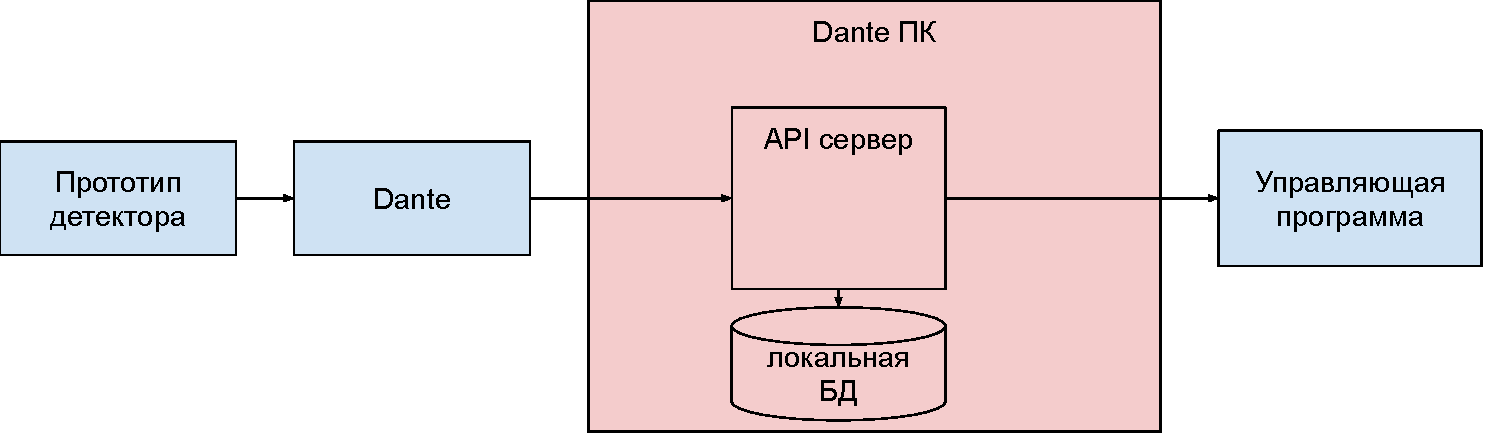
\includegraphics[width = 0.98\textwidth]{img/dante/integration.pdf}
    \caption{Интеграция Dante в систему сбора данных.}
    \label{fig:dante-integration}
\end{figure}

\subsection{Взаимодействие со считывающей системой XGLab}

Устройство для считывания данных детектора Dante представляет собой микросхему, главными элементами которой являются зарядочувствительный усилитель подсоединенный к специализированной интегральной микросхеме, осуществляющей оцифровку и обработку (выделение амплитуды и времени события) сигнала. Взаимодействие с Dante осуществляется посредством TCP/IP сокетов, либо по USB порту с использованием поставляемых с устройством драйверов. Т.к. на момент тестирования существовали только драйвера под Windows, работа с устройством через USB ограничена только этой ОС.

В режиме подключения через TCP/IP Dante предоставляет 4 сокета с буфером размером 4096 байт и портами (8000-8003), первый из которых является управляющим а остальные - передающими. Инициализация подключения всегда осуществляется клиентом. Все команды устройству должны передаваться через управляющий сокет. Ответы от устройства поступают последовательно и упорядоченно на все порты, начиная с 8000 и заканчивая 8003. По утверждению разработчиков это максимизирует пропускную способность устройства. Электроника Dante также имеет возможность может быть объединена в цепь, однако на Троицк ню-масс тестировалось только одиночное подключение.

Устройство имеет 16 байт конфигурационного регистра. Поля регистров делятся на записываемые, читаемые и записываемые и читаемые одновременно. Управление и контроль Dante осуществляется через чтение и запись значений в эти регистры. При этом значения полей сырые, т.е. для записи желаемой конфигурации требуется предварительное кодирование параметров в формат, совместимый с соответствующим полем. Т.к. каждый регистр конфигурации содержит в себе несколько параметров, часто, для задания только одного из них необходимо использовать “безопасную запись”, т.е. запись в 2 этапа: на первом происходит считывание всего регистра, на втором - изменение конкретного бита и запись всего байта обратно в регистр. Расположение регистров указано в таблице \ref{tab:dante-regissters}

\begin{table}
    \centering
    \begin{adjustbox}{width=\textwidth}
        \begin{tabular}{|l|l|l|}
        \hline
        Номер & Название & Описание \\
        \hline
        0 & FIRMWARE\_VERSION & Версия прошивки Dante \\
        \hline
        1 & DPP\_REGISTER\_1 & Конфигурация оцифровки сигнала \\
        \hline
        2 & DPP\_REGISTER\_2 & Конфигурация оцифровки сигнала \\
        \hline
        3 & DPP\_CONFIG\_COMMIT\_OFFSET & Настройка оцифровки (отступы и задержки) \\
        \hline
        4 & ACQUISITION\_STATUS & Параметры набора (старт, стоп и флаг набора) \\
        \hline
        5 & ACQUISITION\_TIME & Задание и считывание времени набора \\
        \hline
        6 & ELAPSED\_TIME & Считывание пройденного времени набора \\
        \hline
        7 & ACQUISITION\_SETTINGS & Выставление параметров набора (режим, маска, биннинг, семплирование) \\
        \hline
        8 & WAVEFORM\_LENGTH & Задание и считывание длины кадра \\
        \hline
        9 & MAP\_POINTS & Конфигурация сообщений для мониторинга набора \\
        \hline
        10 & TIME\_PER\_MAP\_POINT & Конфигурации частоты прихода мониторных данных \\
        \hline
        11 & ETH\_CONFIGURATION\_DATA & Задание и считывание параметров подключения по ethernet \\
        \hline
        12 & Reserved & Зарезервированный регистр \\
        \hline
        13 & ETHERNET\_COMMIT & Задание и считывание параметров подключения по ethernet \\
        \hline
        14 & CALIB\_DONE\_SIGNALS & Считывание информации о калибровке плат \\
        \hline
        15 & Reserved & Зарезервировано для последующих модификаций \\
        \hline
        \end{tabular} 
    \end{adjustbox}
    \caption{Расположение регистров Dante.}
    \label{tab:dante-regissters}
\end{table}

Здесь и во всем бинарном протоколе все биты упакованы в байты с помощью кодировки MSByte.

\subsubsection{Протокол взаимодействия}
Взаимодействие с Dante осуществляется с помощью самодельного бинарного протокола. Каждое сообщение имеет бинарный заголовок размером 8 байт и опциональную часть, содержащую бинарные данные. Сообщения разделяются на команды (посылаемые клиентом устройству) и пакеты (передаваемые устройством на клиент). Оба типа сообщений имеют слегка различные форматы заголовков. Формат команды описан в таблице \ref{tab:dante-command-format}

\begin{table}
    \centering
    \begin{adjustbox}{width=\textwidth}
        \begin{tabular}{|l|l|l|}
            \hline
            Байт & Значение & Описание \\
            \hline
            0 & 0xAA & Спецсимвол начала пакета \\
            \hline
            1 & 0xEE & Спецсимвол начала пакета \\
            \hline
            2 & 0xD + CMD(4 bits) & Код команды \\
            \hline
            3 & Board & Номер платы \\
            \hline
            4 & Packet number & Номер пакета. Используется для трекинга ответов \\
            \hline
            5 & Start address & Адрес регистра Dante к которому применяется команда \\
            \hline
            6 & Length & Количество регистров, к которым применяется команда \\
            \hline
            7 & 0x0 & Зарезервировано для последующих модификаций \\
            \hline
        \end{tabular}
    \end{adjustbox}
    \caption{Формат заголовка команды Dante.}
    \label{tab:dante-command-format}
\end{table}

Сообщение с командой реализует функционал чтения (код команды 0x0) и записи (код команды 0x1) данных из/в регистры конфигурации. 3-й байт в заголовке задает номер платы, к которой будет применена команда. 5-й и 6-й байты задают адрес регистра и количество идущих после адреса регистров, к которым будет применена команда. Оба поля могут содержать значения в диапазоне 0..15. В случае записи, после заголовка должна идти бинарная часть имеющая размер, равный 6-му байту заголовка и содержащая данные для записи в регистры.

Т.к. передача данных по сокету происходит только после записи 2920 байт в буфер, для передачи команды в устройство после записи пакета в поток необходимо также записать в него нули в размере недостающей до 2920 байт части. Только после превышения порога байт сообщение будет отправлено. Формат заголовка пакета указан в таблице \ref{tab:dante-reply-format}.

\begin{table}
    \centering
    \begin{adjustbox}{width=\textwidth}
        \begin{tabular}{|l|l|l|}
        \hline
        Байт & Значение & Описание \\
        \hline
        0 & 0xAA & Спецсимвол начала пакета \\
        \hline
        1 & 0xEE & Спецсимвол начала пакета \\
        \hline
        2 & 0xD + CMD(4 bits) & Код команды \\
        \hline
        3 & Board & Номер платы \\
        \hline
        4 & Packet number & Номер пакета. Такой же, как и в команде \\
        \hline
        5 & Length (High byte) & Размер бинарной части (старший байт) \\
        \hline
        6 & Length (Middle byte) & Размер бинарной части (средний байт) \\
        \hline
        7 & Length (Low byte) & Размер бинарной части (младший байт) \\
        \hline
        \end{tabular}
    \end{adjustbox}
    \caption{Формат заголовка ответного пакета Dante.}
    \label{tab:dante-reply-format}
\end{table}

В случае ответа на команду в 3-м байте будет указан соответствующий команде код. Помимо ответов, в режиме набора данных, Dante будет посылать в одностороннем режиме пакеты, содержащие набранные события. В таких пакетах 4-й байт будет всегда нулевым, а 3-й байт будет иметь значение в соответствии с режимом набора:

\begin{itemize}
    \item 2 - для набора только спектра
    \item 3 - для набора кадров
    \item 4 - для набора событий
    \item 6 - для вывода мониторных данных
\end{itemize}
Байты 5, 6, 7 соответствуют размеру бинарной части пакета (в количестве 32-битных слов)

Формат также подразумевает оборачивание посылаемых сообщений открывающей и замыкающей 2-байтовыми последовательностями имеющими значения 0xDD 0xAA и 0xDD 0x55 соответственно. Если в сообщении имеются байты, совпадающие с одним из байтов открывающей последовательности - они должны быть экранированы с помощью добавления перед каждым из них байта со значением 0xDD.

Пакеты, приходящие с устройства, в отличии от команд, не оборачиваются в открывающие и замыкающие последовательности спецсимволов. Также, к самому пакету не применяется никаких правил экранирования содержимого.

\subsubsection{Настройка платы}

После соединения с Dante и перед запуском набора измерений необходимо провести конфигурацию плат. Для этого в инструкции по разработке платы предоставлена точная последовательность команд, необходимых для установки каждого параметра набора. Эту последовательность необходимо выполнить для всех плат Dante. В процессе настройки будут заданы параметры оцифровки сигнала, такие как инвертирование, время восстановления, режим преобразования амплитуд, порог, время формирования сигнала, порог наложения, ~и т.п. Описанная в мануале последовательность, помимо непосредственно задания параметров описывает способ их кодировки в значения регистров. Команды по заданию параметров также “разбавляются” командами, задающими необходимые программные константные значения битов регистров. Последовательность команд довольно длинная и малопонятная, поэтому ее описание будет опущено.

\subsubsection{Набор амплитуд событий}

В начале тестирования Dante было принято решение сперва отладить процесс набора с оцифровкой сигнала в амплитуды с помощью встроенных в устройство алгоритмов. Для начала набора точки в таком режиме необходимо выполнить следующую последовательность действий:

\begin{enumerate}
    \item Записать в регистр ACQUISITION\_TIME необходимое время набора
    \item Записать в регистры MAP\_POINTS и TIME\_PER\_MAP\_POINT параметры вывода статистики для мониторинга
    \item Записать в регистр ACQUISITION\_STATUS бит, соответствующий старту набора
\end{enumerate}
После выполнения этих действий, Dante в одностороннем режиме начнет посылать сообщения содержащие параметры набранных событий и сообщения, содержащие статистику для онлайн мониторинга набора.

Каждое событие в бинарной части закодировано двумя 32-битными словами в формате, описанном в таблице \ref{tab:dante-binary-word-format}.

\begin{table}
    \centering
    \begin{tabular}{|l|l|p{0.7\textwidth}|}
        \hline
        Слово & Биты & Содержание \\
        \hline
        1 & 31-18 & Время прихода события (14 бит) в 8 нс бинах от начала набора. Младшие биты \\
        \hline
        1 & 17-16 & зарезервировано \\
        \hline
        1 & 15-0 & Амплитуда события (16 бит) \\
        \hline
        2 & 31-30 & Контрольные биты. Для событий значение равно "00" \\
        \hline
        2 & 29-0 & Время прихода события (30 бит) в 8 нс бинах от начала набора. Младшие биты \\
        \hline
    \end{tabular}
    \caption{Формат 32-битного слова в бинарной части пакета Dante.}
    \label{tab:dante-binary-word-format}
\end{table}

Части, содержащие статистические данные имеют фиксированную длину в 32 слова и отделяются от событий 2-мя словами, имеющими контрольные биты со значениями "11", т.е. равные "0xC000000000000000". Т.к. Dante подключается в отладочном режиме, в процессе обработки из бинарных данных сообщения со статистикой просто пропускаются, поэтому описание формата будет опущено.

На рисунке \ref{fig:dante-message} изображена схема бинарного формата Dante.

\begin{figure}
  \centering
  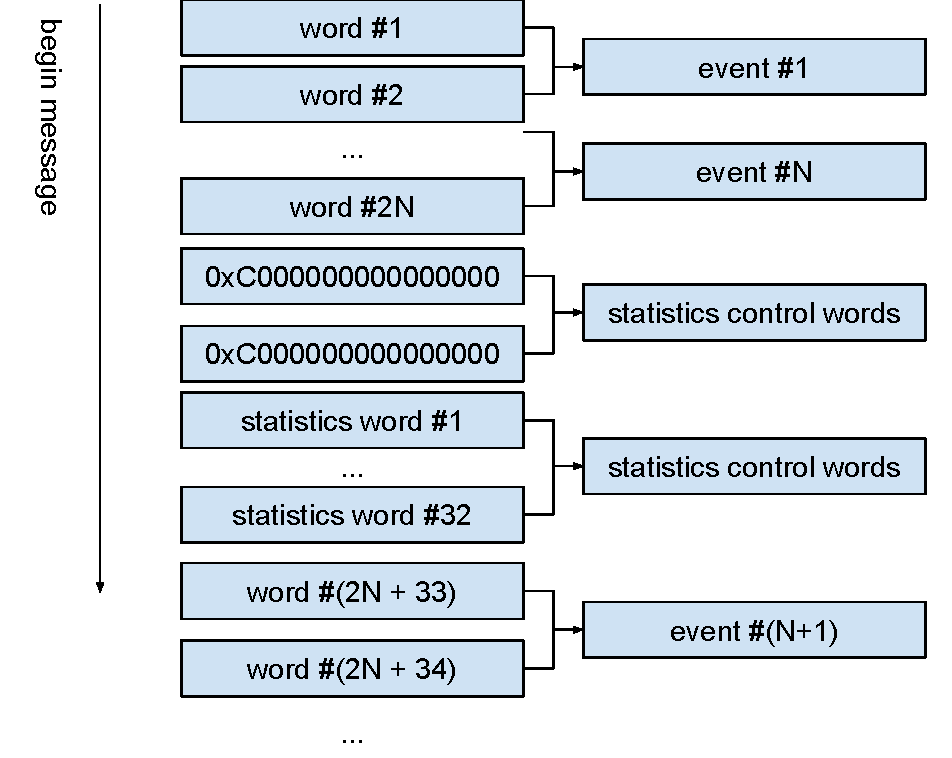
\includegraphics[width = 0.98\textwidth]{img/dante/message.pdf}
    \caption{формат сообщения Dante.}
    \label{fig:dante-message}
\end{figure}

\subsection{Разработка сервиса}
При разработке сервиса для набора событий с помощью Dante было решено использовать режим управления через TCP/IP. На основе модуля python-df-tcp был разработан проект DANTE-server, исходный код которого расположен в репозитории \cite{dante-server}.

Для протокола сообщений Dante был написан парсер. Его код находится в файле protocol.py в корне проекта. Парсер обладает функционалом по созданию сообщений, содержащих команды (экранирование предусмотрено) и пакеты. Также парсер реализует функции по извлечению пакетов из бинарной строки потока.

Файл client.py, расположенный в корне проекта реализует функции по подключению к сокетам Dante, считыванию и склейке пакетов, поступающих от устройства. Код написан с использованием стандартной библиотеки Python 3 asyncio. Скрипт создает 2 очереди:

\begin{itemize}
\item SEND\_QUEUE - используется для передачи команд на Dante
\item GET\_QUEUE - используется для считывания склеенных пакетов с Dante
\end{itemize}
Сам сервис, исходный код которого расположен в файле redirecter.py реализует функции:

\begin{enumerate}
\item Инициализации плат Dante. Инициализация происходит после получения от управляющего компьютера пакета содержащего команду типа init. После получения команды сервер последовательно выполняет набор действий, описанных в руководстве по устройству Dante для каждой из 7 подплат. 
\item Набор точки. Начало набора происходит через запись в описанные в подглаве “Набор амплитуд событий” регистры значений, соответствующих желаемым параметрам набора. После этого программа ожидает приема пакетов. Ожидание по времени составляет время набора плюс константа. Во время ожидания сервер принимает пакеты, вырезает из них статистические данные и извлекает набранные события. Когда время ожидания истекает - сервер считает набор завершенным, компонует полученные события в пакет dataforge-envelope и отправляет их в виде ответа на управляющий компьютер.
\end{enumerate}
Также был разработан виртуальное устройство Dante, которое работает в соответствии с описанном в технической документации поведением. Исходный код виртуального устройства находится в папке test в файле server.py.

\subsubsection{Работоспособность через API}

После создания сервиса Dante, взаимодействующего с устройством через TCP/IP началось тестирование работоспособности такого решения. Для этого проводился набор и анализ данных фоновых событий установки Троицк ню-масс. В процессе тестирования программа провела успешную инициализацию плат Dante и смогла запустить набор событий. Однако набранные файлы, как оказалось, имели нереалистично низкие скорости счета, которые к тому же были нестабильны. Т.к. установка Троицк ню-масс в процессе набора файлов находилась в относительно стабильном режиме, такие эффекты не могли быть вызваны физикой процессов установки. Описанные проблемы не позволяли начинать набор статистики с помощью Dante. Появилась необходимость нахождения причин и устранения ошибок.

Анализ работы разработанного сервера и набранных данных показал следующие моменты:

\begin{enumerate}
    \item Dante перестает работать корректно после переподключения к устройству. 
    \item Если в процессе набора событий приходит команда - устройство зависает. Это исключает возможность проверки завершения набора с помощью регистров.
    \item Время события по видимому записывается не в единицах 8 нс.
    \item Иногда происходит обрезание пакетов (последнее событие пакета имеет размер меньше двух слов)
    \item Иногда Dante начинает присылать пустые события.
    \item Некоторые амплитуды событий имели некорректные значения (больше 16 бит)
\end{enumerate}

Для понимания причин такого поведения сперва было решено перепроверить правильность установки конфигурации при инициализации плат. В комплекте с Dante шло приложение, позволяющее проводить набор данных в ручном режиме через графический интерфейс. Набранные при работе через эту программу файлы выглядели явно лучше чем набранные с помощью сервиса: скорость счета была значительно выше, стабильнее и ближе к ожидаемым значениям. К счастью, через интерфейс программы можно было задать протокол управления: TCP/IP, либо USB. Для проверки корректности работы было решено провести с помощью программы инициализацию плат с помощью TCP/IP и с заранее известными параметрами и с помощью программы Wireshark записать весь трафик, передаваемый на сокеты Dante. Затем, анализируя трафик предполагалось вычленить из него команды и ответы на них и сверить очередность и соответствие ответов с процессом инициализации через разработанный сервис. В процессе анализа трафика оказалось что в работе сервиса действительно присутствовали некоторые ошибки, однако после их устранения желаемой работы устройства все равно не удалось достигнуть. При абсолютно одинаковой последовательности инициализации плат и старта набора данные, набранные разными способами различались.

Вторым этапом была предпринята попытка проведения набора событий с помощью Dante через порт USB. Т.к. идущая в комплекте программа использует именно USB при наборе событий это решение показалось разумным. С помощью стандартного модуля Python ctypes был создан скрипт, проводящий процесс инициализации с помощью драйверов Dante. Однако, при выполнении, скрипт зависал на начальных командах. Возможно это было связано с тем, что поставляемая библиотека общения с драйвером была устаревшая. Т.к. предположительно стандартная программа набора для Dante была написана на LabView такой вариант выглядит реалистичным. Попытки комбинирования протоколов (Т.е. использование TCP/IP для инициализации и USB для набора событий) также не сработало, т.к. устройство, как оказалось, без перезагрузки не может работать одновременно с двумя протоколами.

\subsubsection{Работа через стандартную программу}

В условиях сильной ограниченности по времени было решено отказаться от работы с устройством непосредственно через API и создать новый сервис, который будет привязан к стандартному приложению Dante и проводить набор с помощью эмуляции кликов мыши по графическому интерфейсу (кликер). Это очень не рекомендуемый подход, который имеет очевидные недостатки (привязанность к конкретному разрешению экрана, хрупкость системы, невозможность использовать компьютер во время набора), однако с учетом попыток разбора протоколов взаимодействия такой подход оказался единственным работоспособным вариантом.

Кликер был также написан на Python 3 на основе модуля python-df-tcp. В качестве фреймворка, эмулирующего нажатие мыши был использован модуль PyAutoIt, предоставляющий обертки функций AutoIt\cite{autoit}. Схема набора событий с помощью кликера изображена на \ref{fig:clicker-workflow}.

\begin{figure}
  \centering
  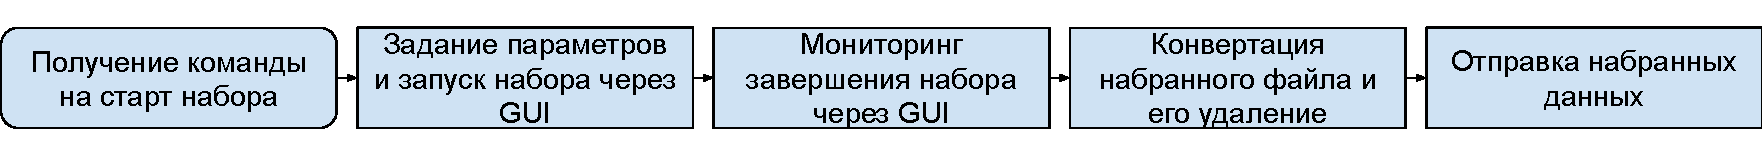
\includegraphics[width = 0.98\textwidth]{img/dante/clicker-workflow.pdf}
    \caption{Cхема работы кликера.}
    \label{fig:clicker-workflow}
\end{figure}

Помимо конфигурации набора, описанного ранее здесь также присутствует этап конвертации данных, полученных стандартной программой в dataforge-envelope формат. Отправляемый сервисом пакет с набранными событиями по структуре очень похож на формат обработанного файла Лан10-12PCI. Бинарные данные пакета имеют одинаковый формат в обоих случаях, метаданные Dante выглядят так:

\begin{lstlisting}[caption={Метаданные пакета с набранными Dante событиями.}, captionpos=b]
{ "start_time": start_time,
  "external_meta": {/*...*/},
  "acquisition_time": 30,
  "type": "reply",
  "reply_type": "aquired_point",
  "status": "ok",
  "time_coeff": 8,
  "total_events": 1000,
  "device": "DANTE daisy chain rev 1.8",
  "dpp_params": {/*...*/}}
\end{lstlisting}

Из отличий от Лан10-12PCI здесь: параметры устройства вынесены из тега "external\_meta" в корень метаданных в тег "dpp\_params", добавлено поле "device", содержащее информацию об устройстве, с помощью которого проводился набор.

\subsection{Результаты тестирования платы}

В процессе интеграции прототипа детектора Katrin с системой считывающей электроники Dante были выявлены следующие проблемы:
\begin{itemize}
    \item Работа в режиме взаимодействия через TCP/IP явно неправильна. Как оказалось, в процессе набора пакеты часто обрезаются и не все события доходят до клиента, а скорость счета сильно изменяется при наборе данных в одинаковых условиях: такая величина изменения не может быть объяснена физическими процессами. Также суммарный объем передаваемых данных, при анализе через Wireshark, оказался намного меньше объема данных, полученных при наборе с помощью стандартных средств, идущих в поставке с Dante. Это говорит о том, что ошибка передачи событий происходит внутри самого устройства и не может быть объяснена ошибками парсинга, связанными с обработкой битых пакетов. В дополнение неясно использование 4 сокетов - не очевидно, что это может максимизировать пропускную способность с учетом того, что к устройству можно подсоединить только один ethernet кабель. 
    \item Поставляемые с Dante драйвера для работы с USB по видимому устаревшие. В процессе их тестирования не удалось добиться инициализации подплат - вызов функций библиотеки драйвера приводит к зависанию программы. Этот и предыдущий пункты приводят к необходимости использования стандартной программы для взаимодействия с Dante. При работе на установке Троицк-ню масс для обхода этих проблем был использован кликер - такое решение подходит для тестирования, однако на реальных сеансах Katrin, особенно с учетом высоких требований к скоростям счета, такой метод неприемлем.
    \item Работа с устройством по API требует задания низкоуровневых настроек через регистры, кодирования параметров набора в приемлемые для них форматы и задания “магических” констант. Такое задание явно не удобно и, с учетом потенциальной стоимости Dante, может быть легко и без сильного удорожания решено добавлением к устройству микрокомпьютера, который будет производить конвертацию внутренних команд и ответов Dante в высокоуровневый и понятный формат.
\end{itemize}

\chapter{Обработка непрерывного сигнала}
При переходе на поиски стерильного нейтрино в диапазоне энергий до 5 кэВ появляется проблема обработки высоких скоростей счета детектора\cite{2015JInst..1010005A}. Согласно предложениям, для успешной работы система должна справляться со скоростями порядка 40-50 кГц, иметь хороший алгоритм разделения наложений и точно определять мертвое время (не менее 100 нс неопределенности). Детектор, в текущей конфигурации системы сбора данных генерирует сигналы с длиной около 4 мкс. При такой длине, используемая раньше система обработки сигнала и регистрации событий перестает справляться и может проводить разделение с описанными требованиями. Поэтому было решено провести обновление аппаратной части, заменить старую аппаратную оцифровку на плату Лан10-12PCI, набирать с помощью нее квазинепрерывный сигнал и программно выделять из него параметры событий. При таком подходе скорость счета определяется качеством разделения наложенных событий. 

На момент разработки существовало несколько способов разделения. Например, коррекция амплитудного спектра с помощью нейронный сетей. Алгоритм описан в  \cite{2017JHEP...12..051K} использует смоделированные спектры в качестве обучающей выборки, а затем использует полученную сеть для анализа данных. Недостаток этого подхода заключается в том, что он требует знания формы исходного неискаженного спектра амплитуд для правильной процедуры обучения. Также любые аномалии в распределении времени события могут привести к неверным результатам коррекции.

Другой способ описан в \cite{2013NIMPA.717...21C}. Он основан на аналитической модели, которая предсказывает мертвое время и искажения спектра, вызванные наложениями сигналов. Несмотря на хорошие результаты, модель жестко привязана к аналитической формуле импульса и поэтому неприменима в других системах без существенных изменений.

Предлагаемые нами алгоритмы коррекции также основаны на форме отдельного события. Однако вместо использования априорной информации, такой как форма спектра или формула аналитического сигнала, он опирается только на данные непрерывного сигнала, собранные с АЦП, и извлекает все необходимые параметры из них. Это делает алгоритмы применимыми для различных задач оцифровки сигнала без существенных изменений.

\section{Характеристики Лан10-12PCI}

\begin{figure}
  \centering
  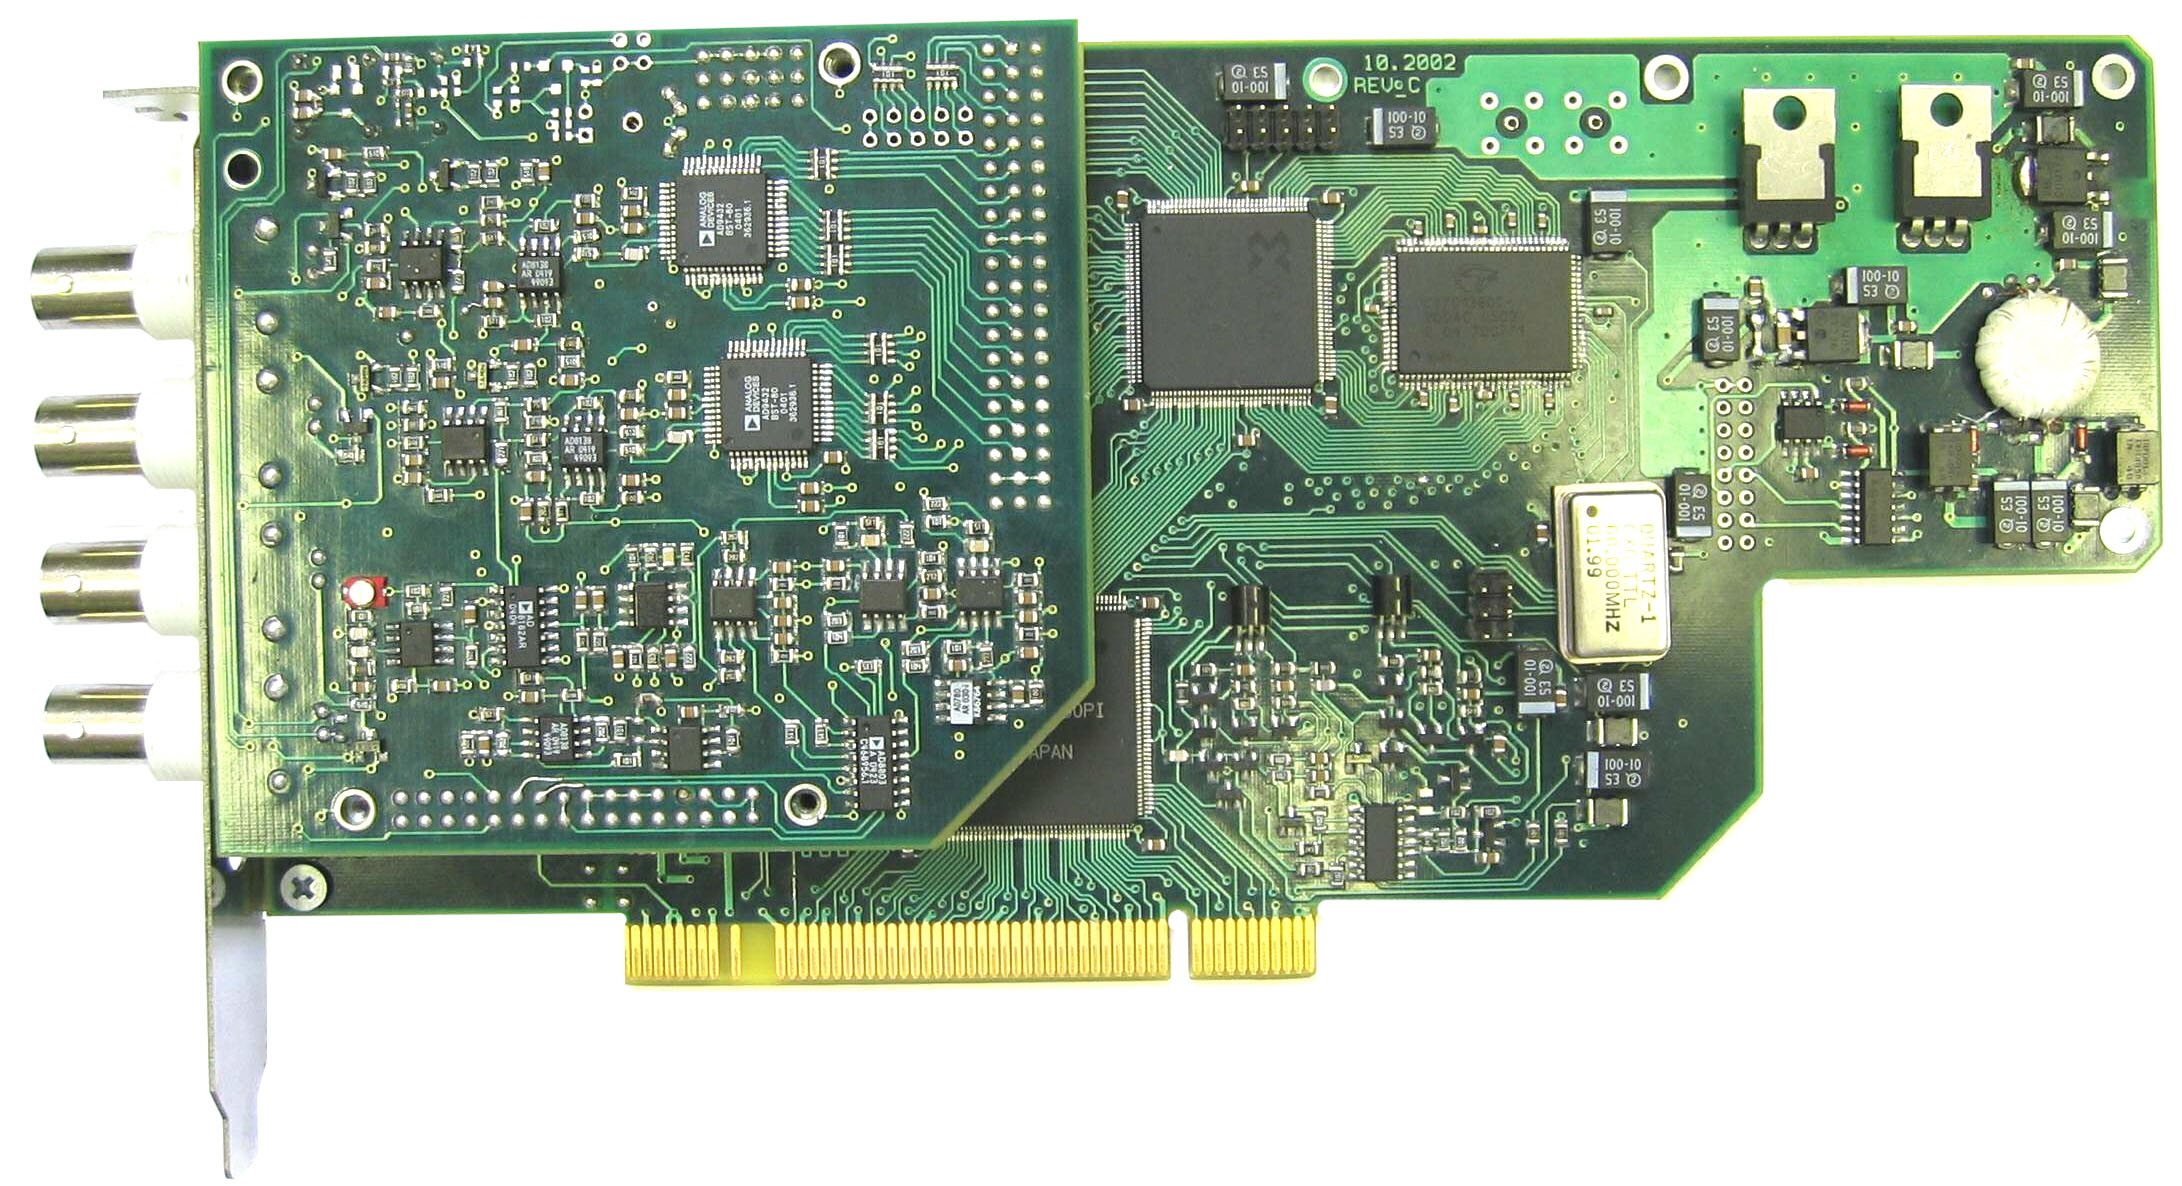
\includegraphics[width = 0.7\textwidth]{img/signals/Lan10-12PCI.jpg}
    \caption{Плата Лан10-12PCI.}
    \label{fig:lan10-view}
\end{figure}

Плата произведена ЗАО {\textquotedbl}Руднев-Шиляев{\textquotedbl} и представляет собой встраиваемый в ПК через PCI 12-битный АЦП. Лан10-12PCI имеет 2 аналоговых входа, канал внешней синхронизации и канал внешней тактовой частоты. Возможные частоты дискретизации составляют от 100 МГц до 6.1035 кГц или любая частота в диапазоне от 5 МГц до 100 МГц при работе с внешней тактовой частотой. Возможные длины - от ~28 до 220бинов на кадр. Имеется внутренний буфер размером 512 кб, который может одновременно хранить один кадр вне зависимости от его размера. Запись кадров может проводиться в трех режимах

\begin{enumerate}
    \item По превышению порога
    \item По событию канала внешней синхронизации
    \item По программному триггеру (через API)
\end{enumerate}
Подробные характеристики можно найти в .

Плата была выбрана в основном из-за ее низкой цены, однако для нашей задаче она имеет некоторые преимущества. Это:

\begin{enumerate}
    \item Наличие относительно большого внутреннего буфера и возможность ручного считывания кадра по программному триггеру.
    \item Наличие комплектных драйверов для Windows и Linux и полноценного API к ним.
\end{enumerate}
Перед интеграцией платы было проведено тестирование набора кадров в режиме записи по превышению порога. Результаты представлены в таблице \ref{tbl:lan-cr}.

\begin{table}
\centering
    \caption*{Размер кадра - 1 мкс}
    \begin{tabular}{|l|l|l|}
        \hline
        Частота, кГц & Эффективная частота, кГц & Эффективность \\
        \hline
        40 & 2,553 & 0,064 \\
        \hline
        20 & 2,554 & 0,128 \\
        \hline
        5 & 2,558 & 0,512 \\
        \hline
        1,25 & 1,242 & 0,993 \\
        \hline
    \end{tabular} 

    \caption*{Размер кадра - 2 мкс}
    \begin{tabular}{|l|l|l|}
        \hline
        Частота, кГц & Эффективная частота, кГц & Эффективность \\
        \hline
        40 & 2,489 & 0,062 \\
        \hline
        20 & 2,537 & 0,127 \\
        \hline
        10 & 2,527 & 0,253 \\
        \hline
        1,25 & 1,238 & 0,99 \\
        \hline
    \end{tabular} 

    \caption*{Размер кадра - 4 мкс}
    \begin{tabular}{|l|l|l|}
        \hline
        Частота, кГц & Эффективная частота, кГц & Эффективность \\
        \hline
        40 & 0,464 & 0,012 \\
        \hline
        10 & 0,918 & 0,092 \\
        \hline
        2,5 & 0,788 & 0,315 \\
        \hline
        0,313 & 0,31 & 0,992 \\
        \hline
    \end{tabular}
    \caption{Эффективность Лан10-12PCI при наборе по триггеру}
    \label{tbl:lan-cr}
\end{table}

Тестирование показало что даже при минимальном размере кадра, эффективная скорость счета составляет примерно 3-4 кГц, что совершенно не соответствует требованиям для системы сбора данных установки. Дальнейшее тестирование показало, что основной вклад в мертвое время дает сброс данных из внутреннего буфера платы на ПК. Т.о. существует возможность оптимизации набора с помощью минимизации количества сбросов буфера платы.

\section{Набор непрерывного сигнала}

Для минимизации количества сбросов мы выставляем максимальную длину кадра в $ 2^{20} $ и проводим непрерывный набор по программному триггеру, который генерируется  сразу после считывания предыдущего кадра из буфера АЦП. Т.о. с платы считываются длинные кадры (размер кадра намного больше  размера события) без привязки к событиям. На рисунке \ref{fig:lan10-signal-acq} представлена описанная схема набора.

\begin{figure}
  \centering
  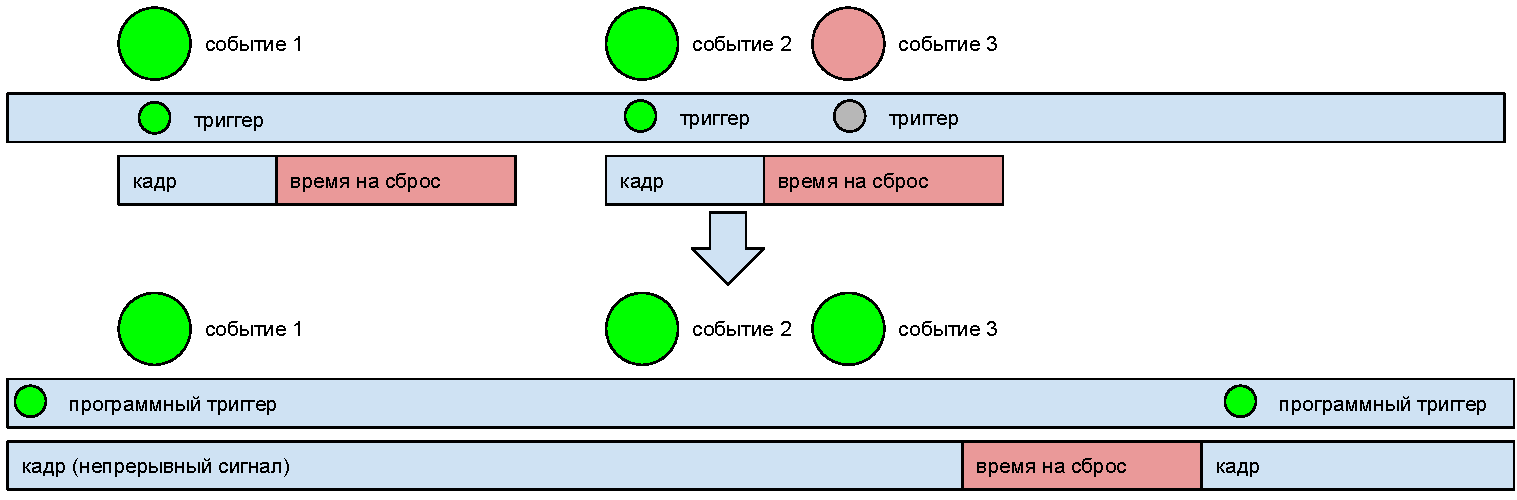
\includegraphics[width = 0.7\textwidth]{img/signals/signal-acq.pdf}
    \caption{Набор кадров по триггеру (сверху) и квазинепрерывного сигнала по программному триггеру (снизу).}
    \label{fig:lan10-signal-acq}
\end{figure}

На выходе мы имеем практически непрерывную сигнал с разрывами только на сброс данных, которые заранее определены и могут быть учтены при обработке как живое время. Т.о. данные не содержат искажений, обусловленных аппаратным мертвым временем. Извлечение параметров событий перекладывается с аппаратной составляющей платы, которая в нашем случае сильно ограниченна, на ПК. Т.о. скорость обработки ограничивается только параметрами компьютера (также обработка может быть отложенной, если ресурсы не позволяют делать ее в реальном времени). 

Для Лан10-12PCI описанный метод набора был исследован на некоторых частотах оцифровки. Параметры живого времени для разных частот дискретизации приведены в таблице \ref{tab:lan-cr-cont}. Видно, что операция переноса занимает одинаковое время для любого размера кадра. Для набора экспериментальных данных была выбрана частота оцифровки - 3.125e+6 Гц (320 нс). При такой частоте плата обеспечивает 87\% живого времени и дает оптимальное соотношение размеров набираемых файлов и спектрального разрешения.

\begin{table}
    \centering
    \begin{adjustbox}{width=\textwidth}
        \begin{tabular}{|p{0.20\textwidth}|p{0.25\textwidth}|p{0.10\textwidth}|p{0.20\textwidth}|p{0.20\textwidth}|}
            \hline
            Частота оцифровки, Гц & мертвое время за 10 с набора, с & кол-во кадров & время на запись кадра, с & Эффективность записи, \% \\
            \hline
            1.25e+7 & 3.96 & 72 & 0.055 & 0.604 \\
            \hline
            6.25e+6 & 2.45 & 45 & 0.054 & 0.755 \\
            \hline
            3.125e+6 & 1.28 & 26 & 0.049 & 0.872 \\
            \hline
        \end{tabular}
    \end{adjustbox}
    \caption{Эффективность Лан10-12PCI при наборе квазинепрерывного сигнала }
    \label{tab:lan-cr-cont}
\end{table}

\subsection{Предобработка данных}
Для экономии места жесткого диска, из набираемых кадров, содержащих непрерывный сигнал, вырезаются только интервалы, содержащие события. Обрезание производится с помощью алгоритма zero-suppression. Алгоритм фильтрует все бины, имеющие амплитуду ниже порога и не имеющие соседних бинов выше порога в заданной окрестности, вырезаются. Т.о. сигнал разбивается на кадры переменной длины, содержащие события.

\begin{figure}
  \centering
  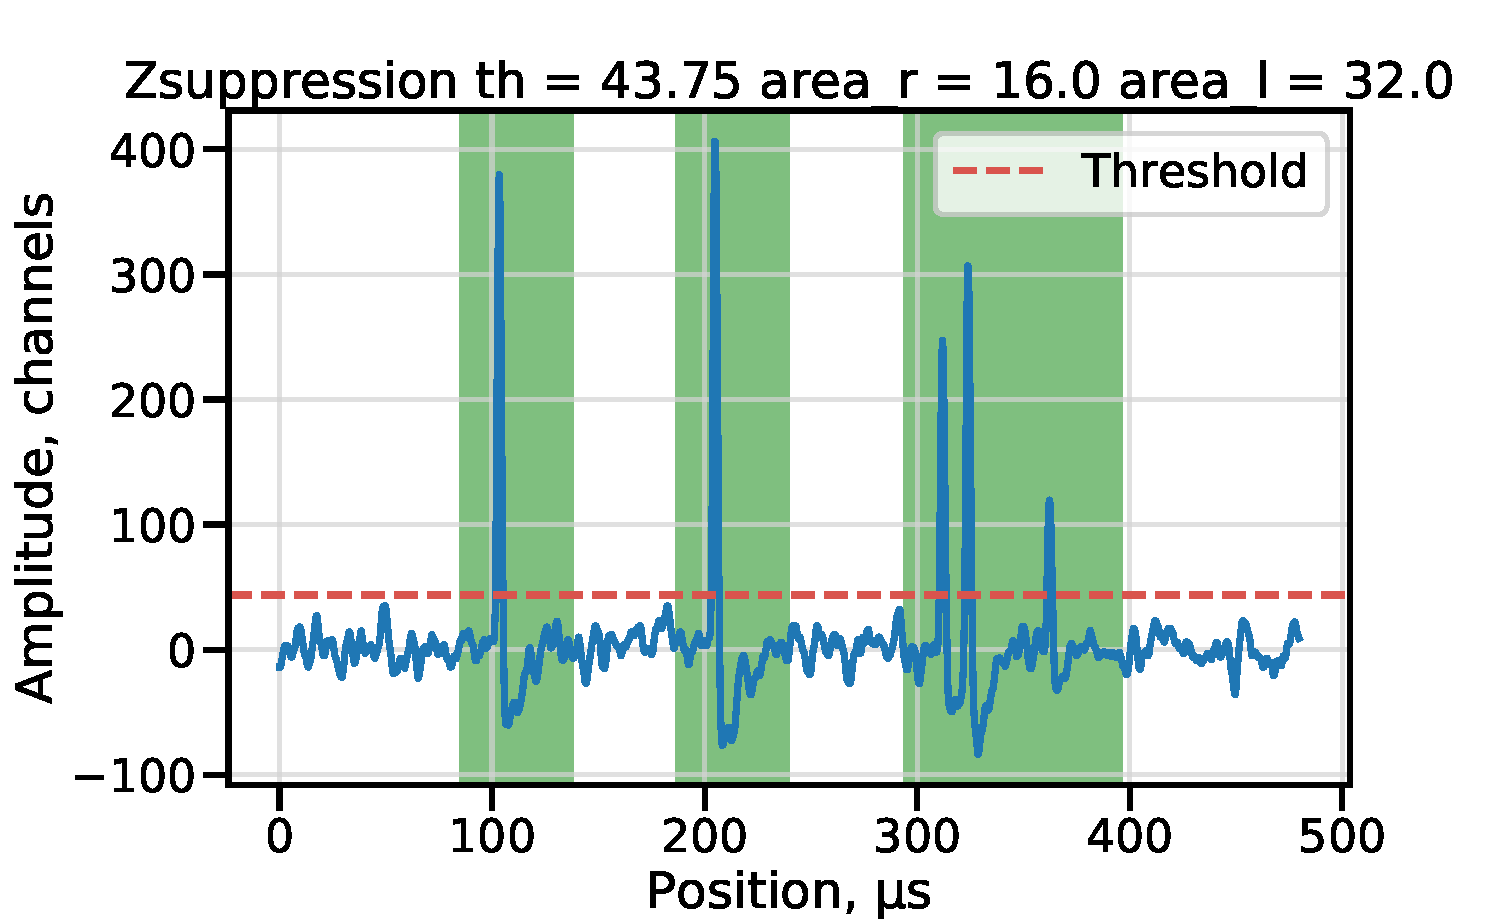
\includegraphics[width = 0.99\textwidth]{img/signals/zsuppression.pdf}
    \caption{Алгоритм zero-suppression.}
    \label{fig:signals-zsuppression}
\end{figure}

Алгоритм операции zero-suppression:
\begin{enumerate}
    \item Создание маски
    \begin{enumerate}
        \item Бинаризация кадра по пороговому значению
        \item Применение морфологической диляции с ядром, соответствующем желаемым границам события
    \end{enumerate}
    \item Вырезание отфильтрованных участков по созданной маске
\end{enumerate}

Данная реализация позволяет избежать дублирования пограничных областей событий за счет слияния близких событий в один подкадр. Далее в работе для простоты мы будем ссылаться на подкадр, полученный в результате предобработки ~алгоритмом zero-suppression, как простой «кадр» и «кадр непрерывного сигнала» - для исходного кадра Лан10-12PCI до предобработки.

\section{Симуляция непрерывного сигнала}

Для разработки и тестирования алгоритмов выделения параметров событий требуется большая промаркированная выборка кадров непрерывного сигнала. Единственным реальным способом его получения является моделирование. В ходе работы мы разработали генератор данных платы Lan10-12PCI, который создает непрерывные кадры сигнала, имитирующие вывод реального устройства. Для создания события в кадре генератор использует два определяющих параметра - амплитуду и время. Поскольку параметры определены явно, кадры непрерывного сигнала создаются уже размеченными. Вывод генератора рассчитан на полную совместимость с выводом реальной платы. Такой подход к генератору имеет свои преимущества и недостатки. С одной стороны, сырой вывод платы является первичным входом для всей системы обработки, использование таких сгенерированных размеченных данных позволяет протестировать все этапы обработки. Кроме того, нет необходимости разрабатывать дополнительный код тестирования (все манипуляции с данными будут такие же как и для реальных измерений). Еще одним преимуществом является возможность разработки без самой платы, поскольку генератор также можно использовать в качестве виртуального устройства. Недостатком является необходимость выполнения всех этапов обработки для тестирования любой компоненты. Это значительно снижает скорость тестирования (особенно для конечных этапов обработки) по сравнению со случаем генерации данных для конкретного этапа. Также может появиться узкое место

в случае, если некоторые промежуточные этапы занимают намного больше времени, чем тестируемый. 

Архитектурно, наш генератор данных состоит из двух модулей:

\begin{itemize}
    \item Генератор шумов
    \item Генератор форм событий
\end{itemize}
Непрерывный сигнал получается путем наложения чистых форм событий на шумовой фон.

\subsection{Моделирование шумового фона}

Мы предполагаем, что шум состоит из большого количества низкоамплитудных событий, равномерно распределенных по времени и имеющих ту же форму, что и физическое событие. Таким образом, шум может быть создан путем явного наложения форм, созданных чистым генератором форм событий без дополнительных модулей. Однако, чтобы ускорить симуляцию, можно оптимизировать генерацию шума.

Принимая во внимание высокую частоту и распределение пиков фоновых событий, можно генерировать конечную форму наложенных шумовых событий с помощью метода, основанного на применении композиции операций сглаживания к массиву случайных чисел.

Алгоритм генерации шума тогда работает следующим образом:

\begin{enumerate}
    \item Создание массива случайных чисел с равномерным распределением. Размер массива равен размеру выходного кадра.
    \item Размытие массива с большим константин ядром для достижения среднего числа пиков, аналогичных реальному шуму. Грубая подстройка распределения амплитуд шума.
    \item Двойное размытие массива с небольшими константными ядрами для достижения необходимого размытия небольших пиков. Тонкая подстройка распределения амплитуд шума.
    \item Округление значений массива до целого числа и сдвиг их значений на 2 бита, для обеспечения соответствия 12-битным значениям полученным реальной платой.
\end{enumerate}
Этот алгоритм позволяет генерировать с небольшими затратами суммарную форму от большого количества равномерно и плотно распределенных по времени событий. В отличие от метода наложения событий, результирующий кадр не будет размечен, но он приемлем для шума.

Для проверки генератора шума, мы сравнили смоделированный шум с реальным. Настоящий шум был получен путем комбинированием небольших фрагментов, оставленных алгоритмом zero-suppression до события. Размеры ядра свертки были подобраны вручную. При подборе мы наблюдали за:

\begin{enumerate}
    \item Соответствием амплитудных спектров реального и генерируемого шума.
    \item Визуальным совпадением формы шумовых пиков и средних расстояний между соседними пиками для некоторых случайно выбранных фрагментов.
\end{enumerate}

\begin{figure}
  \centering
  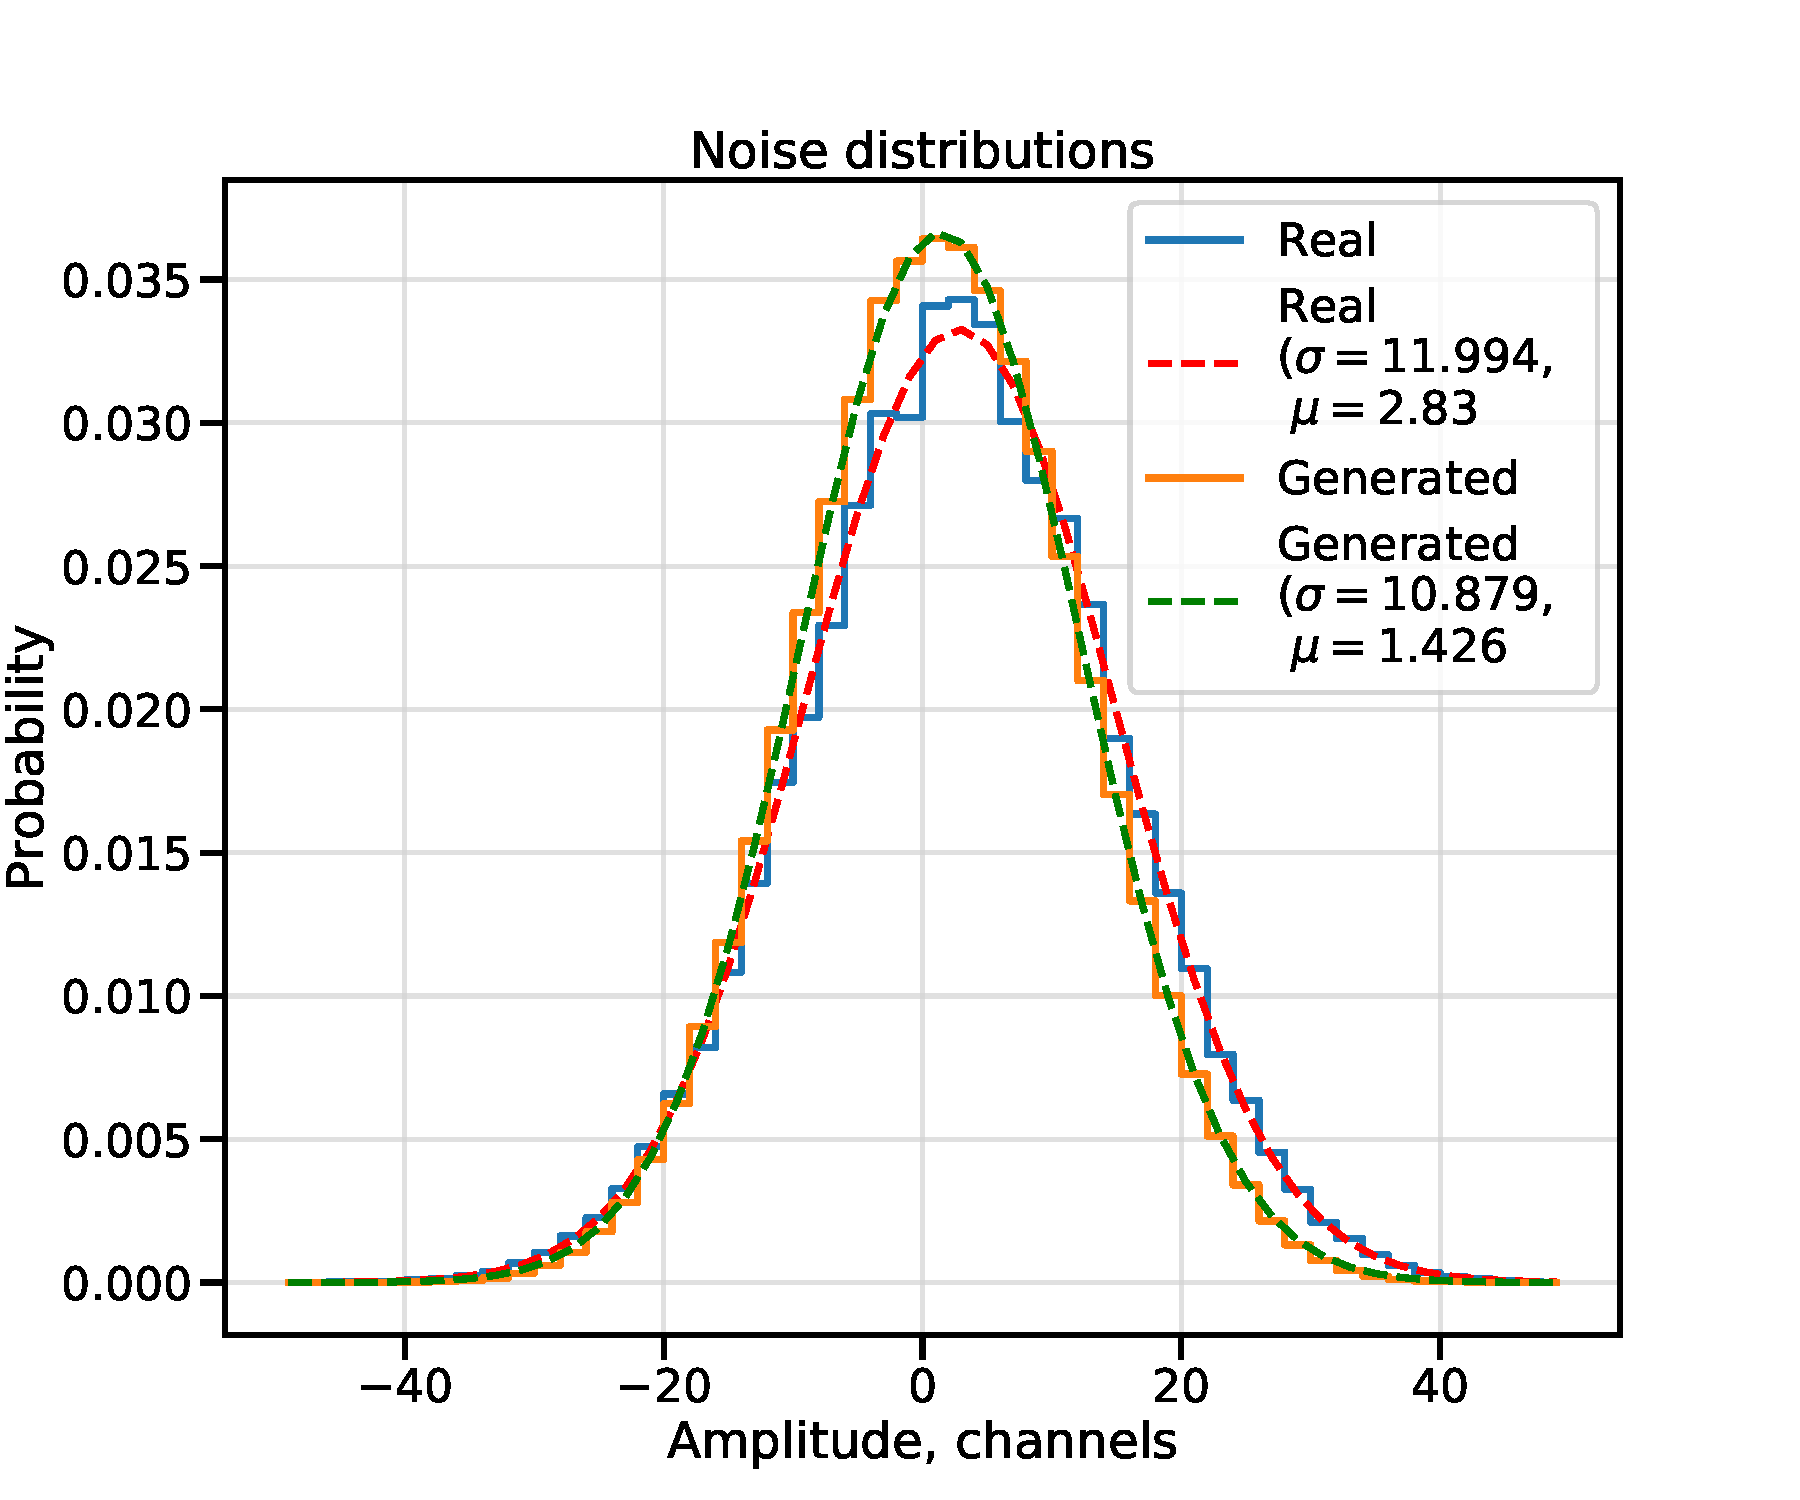
\includegraphics[width = 0.99\textwidth]{img/signals/noise_dist_2017_05.pdf}
    \caption{Сравнение шумовых спектров.}
    \label{fig:signals-noise-dist}
\end{figure}

Как видно по изображенным на \ref{fig:signals-noise-dist} распределениям базовая линия может колебаться между сериями измерений. Тестирование проводилось на более поздних наборах данных и мат. ожидание для шумов сместилось на примерно на 12 каналов. Однако статистические параметры шумов находятся близко друг с другом. Далее будут приведены результаты тесты выделения событий с различными значениями генератора шумов.

Также теперь известны мат. ожидание и среднеквадратичное отклонение для распределения амплитуд шумов, которое понадобится нам при анализе формы.

\subsection{Моделирование формы события}
Чтобы смоделировать событие, необходимо знать его реальную, не искаженную шумами форму. Формы событий могут быть извлечены из данных путем группировки событий по значению амплитуды и последующего усреднения форм по группам. Размер кадра после обрезки также дает предварительное условие, которое может отфильтровывать кадры с наложениями.

\begin{figure}
  \centering
  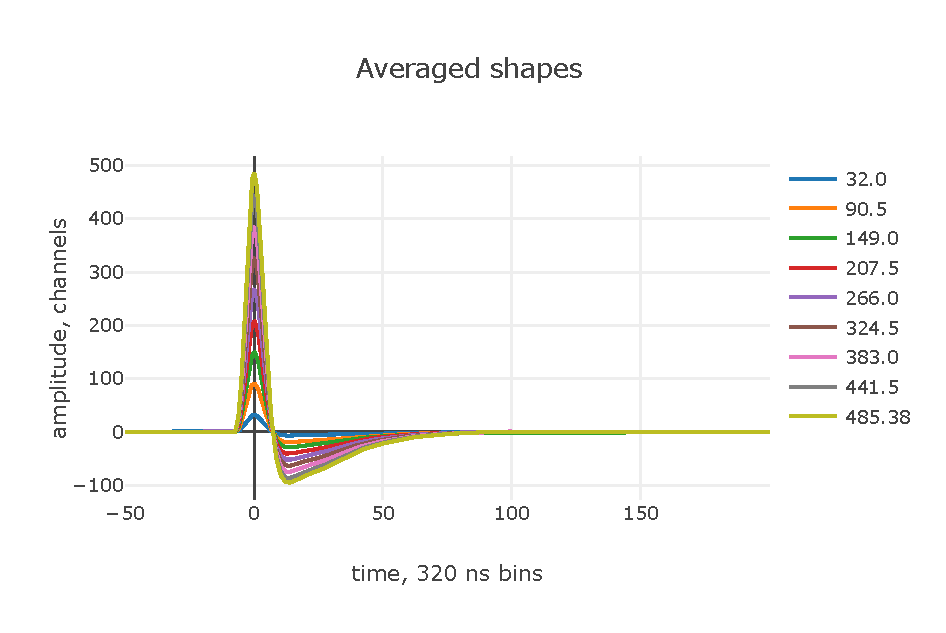
\includegraphics[width = 0.99\textwidth]{img/signals/event_shapes_2017_05.pdf}
    \caption{Усредненные формы событий.}
    \label{fig:signals-event-shapes-05}
\end{figure}

Результаты усреднения событий по группам показаны на рисунке \ref{fig:signals-event-shapes-05}. По внешнему виду форм видны следующие особенности:
\begin{enumerate}
    \item Пик события хорошо описывается гауссианом.
    \item Выброс после события после достижения максимума экспоненциально затухает.
    \item Соотношение между амплитудами пика и выброса постоянно.
    \item Также постоянно расстояние между экстремумами пика и выброса.
\end{enumerate}

Для нашей конкретной формы была подобрана аналитическая кусочно-заданная функция \ref{eq:shape_formula}.

\begin{equation}\label{eq:shape_formula}
    \begin{split}
    & t_f = 2.9604, p = 2.2056, t_a = 0.3701, \\
    & \sigma = 0.3416, f_b = 3.125e+6, \\
    & g(x) = exp(-\frac{|\sigma f_b x|^p}{2}), g_r(y) = \frac{(-2 log(y))^{1/p}}{\sigma f_b}, \\
    & s(x) = \begin{cases}
    & (\frac{1}{(1 + 2 x f_b s)^{t_f}} - 1) exp(-x f_b s), x > 0 \\
    & 0, x \leq 0 \\
    & \end{cases}, \\
    & S(x, a, o) = (g(x - p) + s(x - g_r(0.1) - p) t_a ) a. \\
    \end{split}
\end{equation}

Здесь $g(x)$- Гауссова функция, $ g_r(y) $ - обратная Гауссова функция (только правая часть), $ s(x) $ - функция, описывающая выброс. Константы подобраны фитированием. Объясним формулу. Начало и пик и неполная часть спада события описывается только функцией Гаусса, т.е $g(x)$. На спаде, в месте, где амплитуда переходит порог равный 10 \% от максимальной амплитуды, к Гауссиану добавляется хвост, выраженный функцией $ s(x) $. Для вычисления пороговой точки используется обратный Гауссиан $ g_r(y) $. Наконец, переменные $ a $ и $ p $ в формуле $ S(x,a,p) $ задают амплитуду (задается линейно) и отступ от начала кадра соответственно.

\begin{figure}
  \centering
  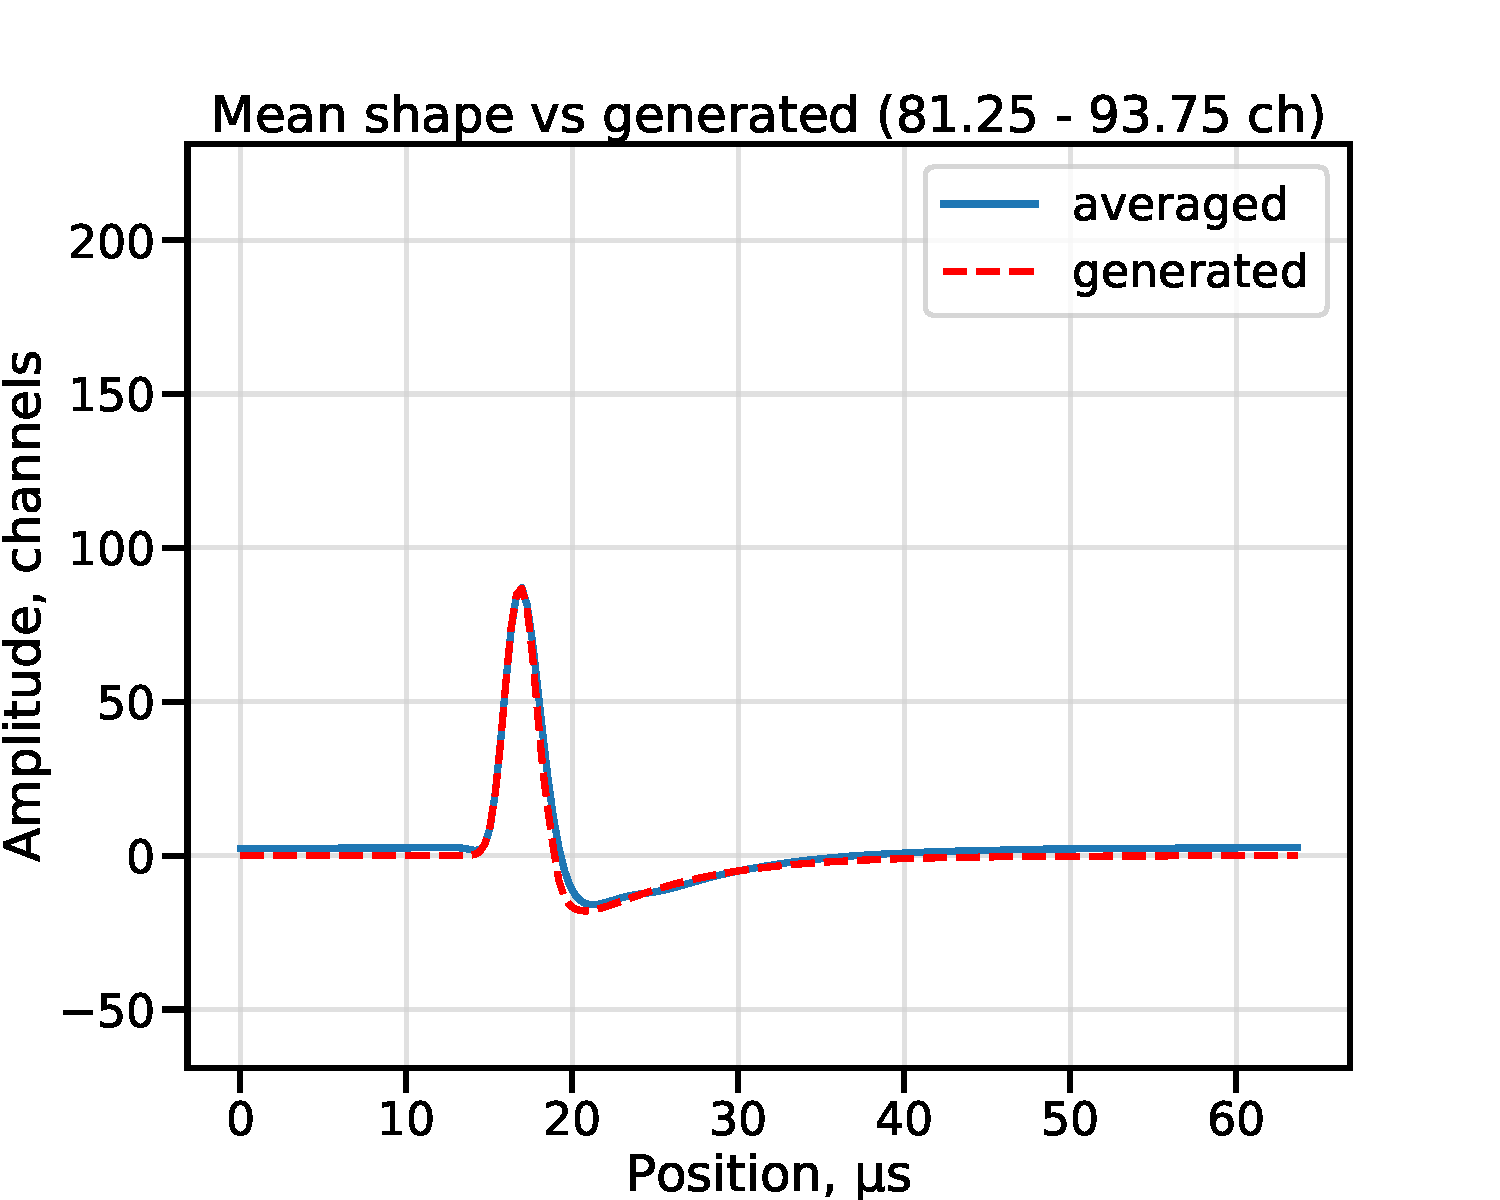
\includegraphics[width = 0.45\textwidth]{img/signals/shapes/1.pdf}
  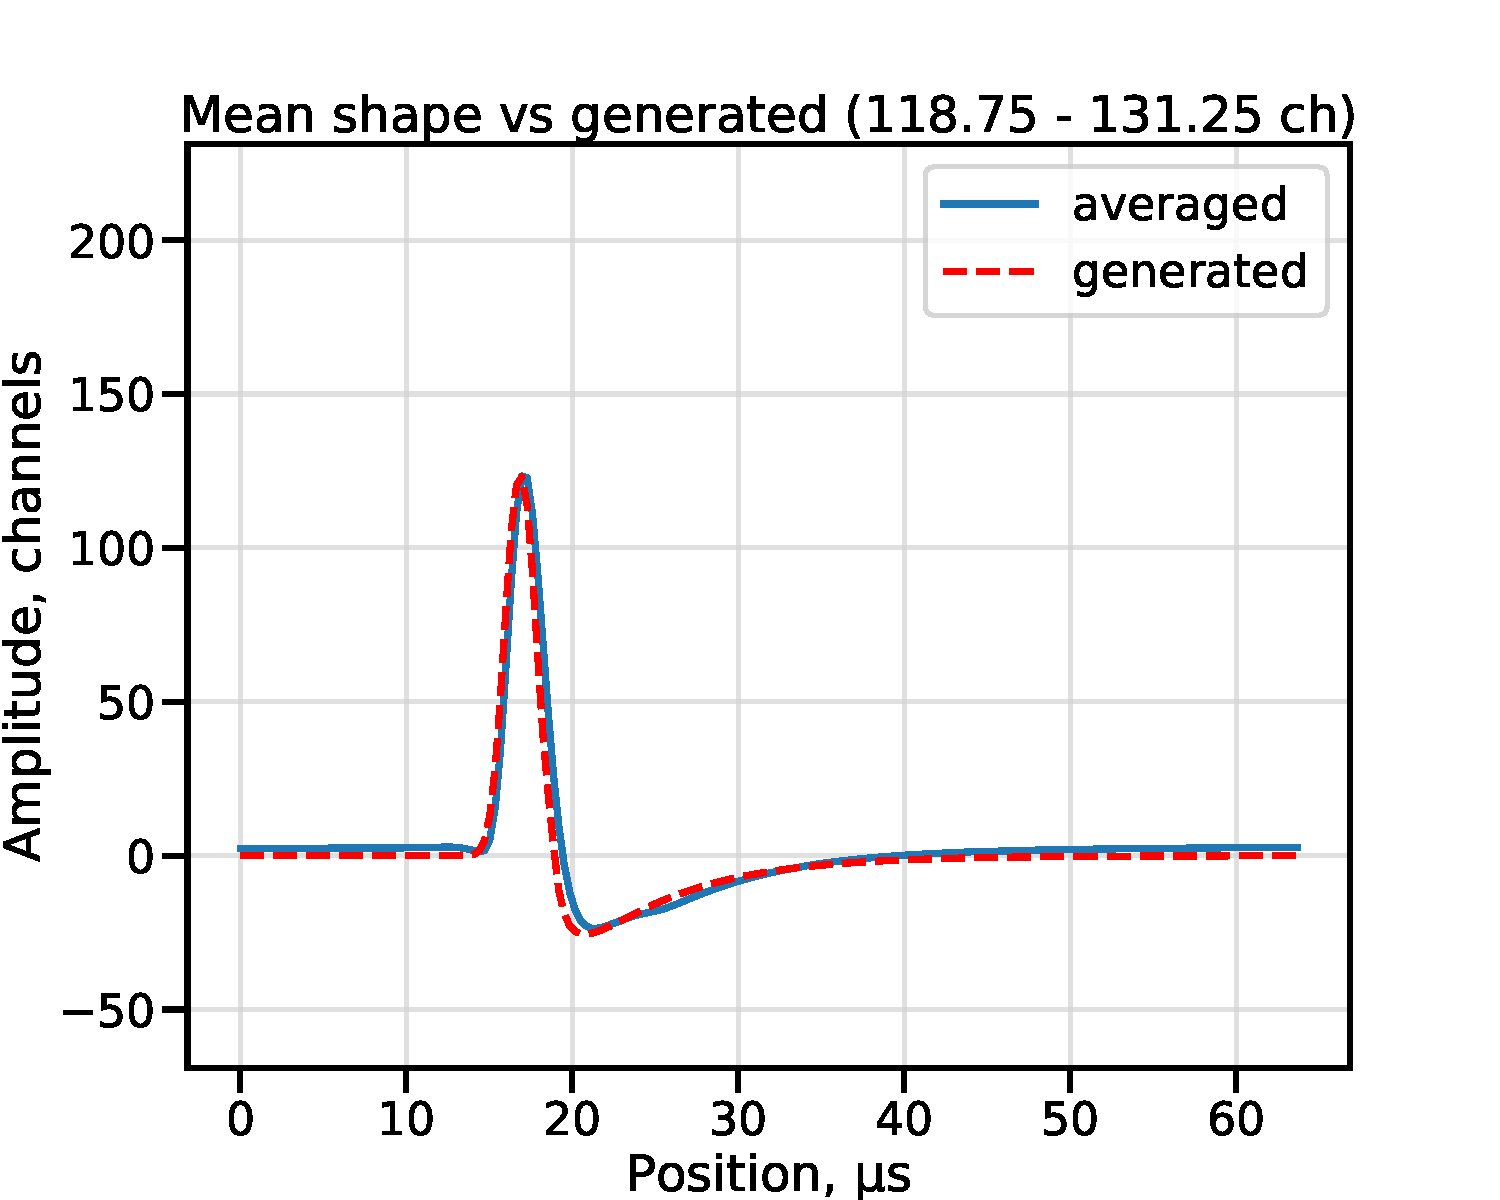
\includegraphics[width = 0.45\textwidth]{img/signals/shapes/2.pdf} \\
  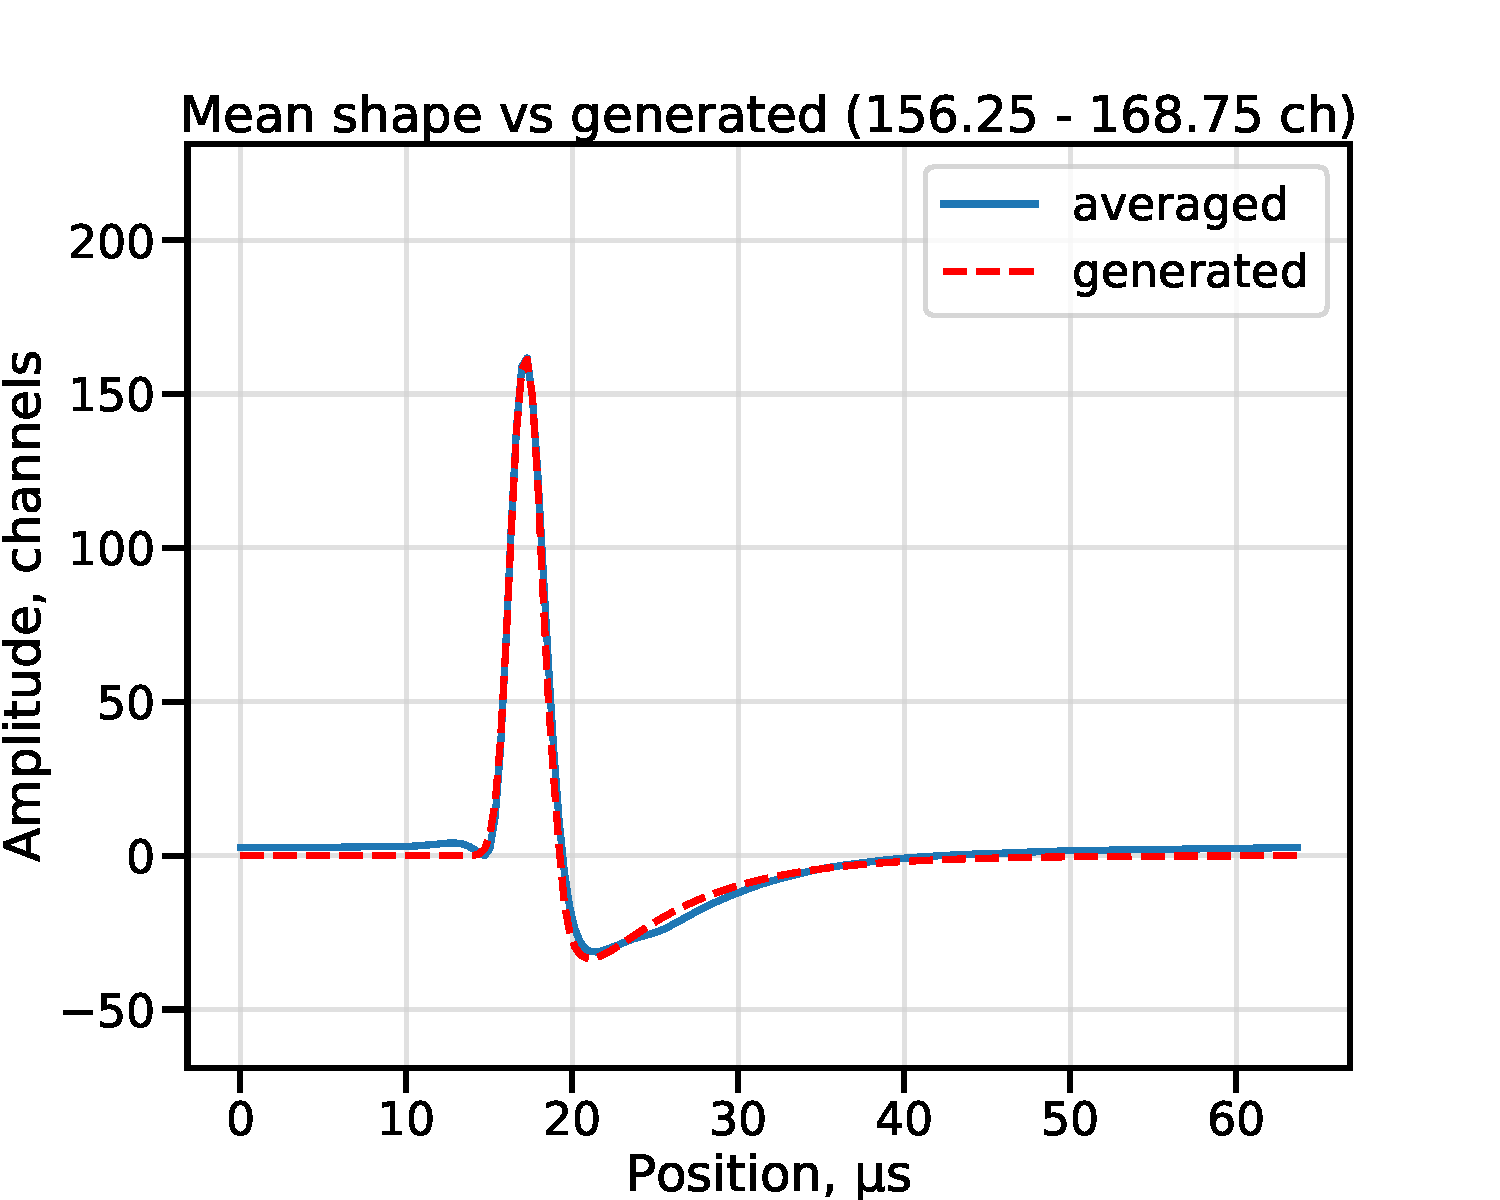
\includegraphics[width = 0.45\textwidth]{img/signals/shapes/3.pdf} 
  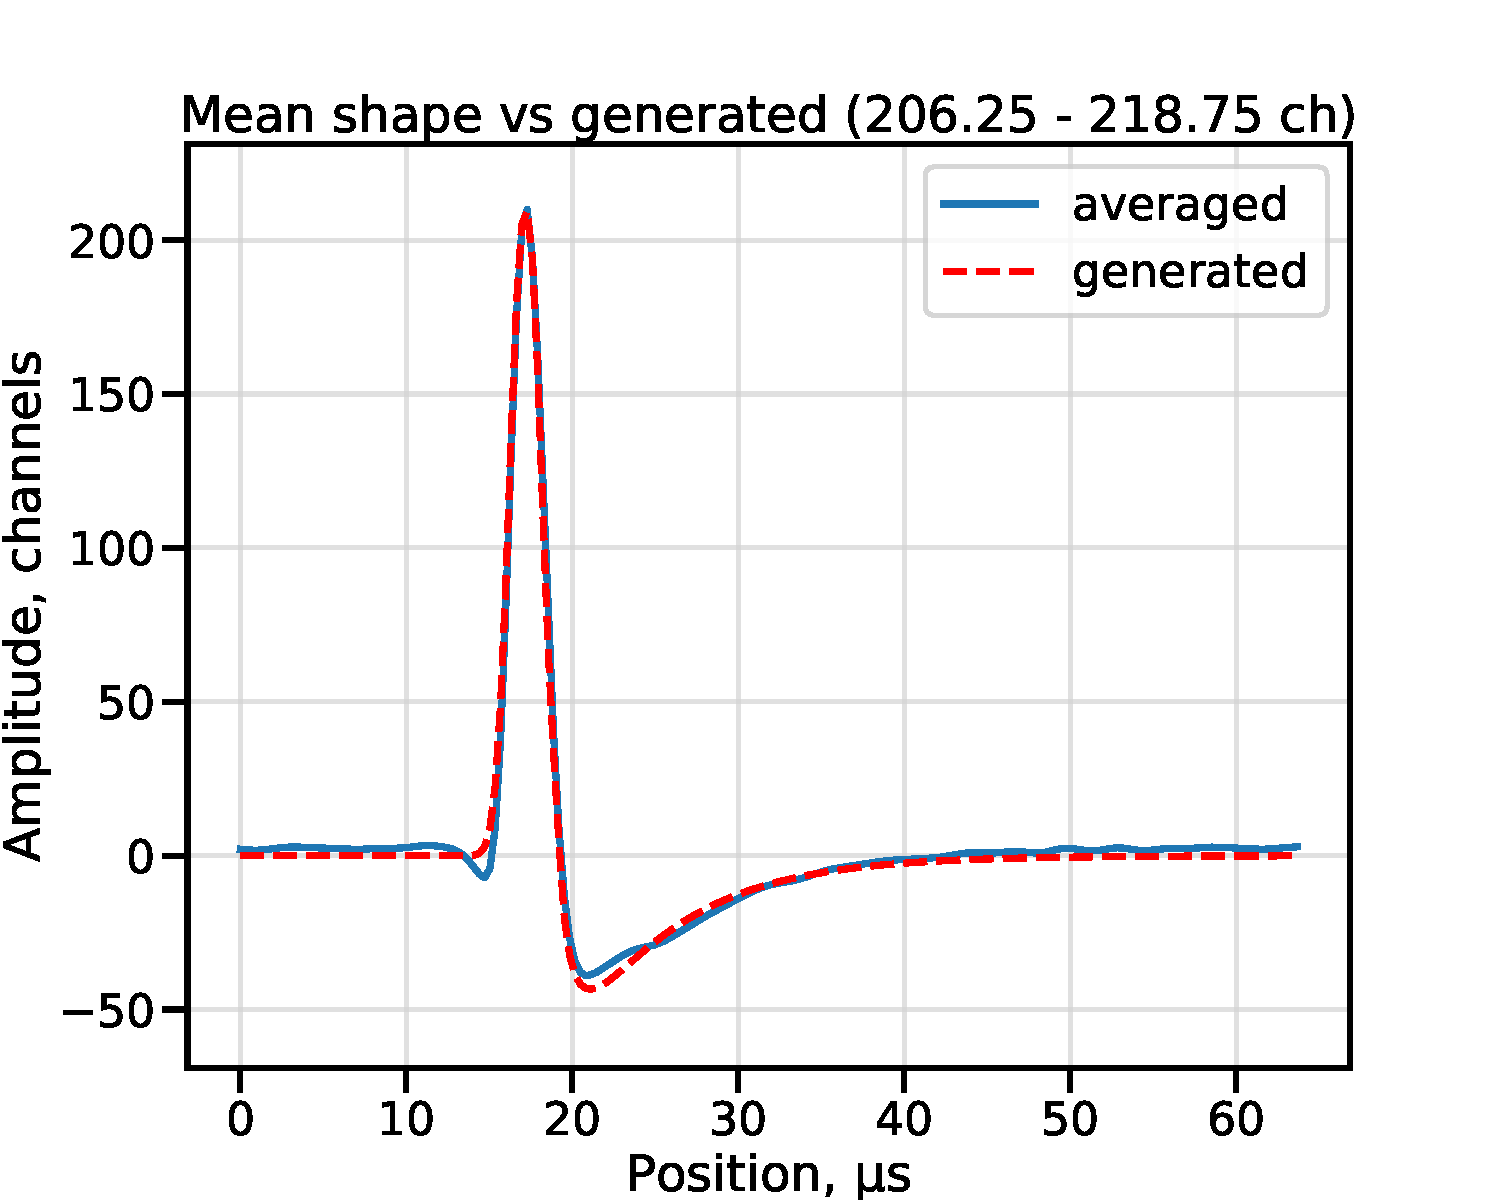
\includegraphics[width = 0.45\textwidth]{img/signals/shapes/4.pdf}
  \caption{Сравнение аналитической у реальной усредненной форм для разных амплитуд.}
  \label{fig:signal-shapes}
\end{figure}

На рисунке \ref{fig:signal-shapes} показаны результаты фита функции события на усредненную форму для нескольких амплитуд.Видно, что подобранная функция хорошо описывает реальное событие.  

\subsection{Валидация генератора}\label{generator-validation-1}

Для проверки соответствия реальных и полученных генератором кадров были построены распределения квадратичных отклонений форм восстановленных событий. Для этого для двух типов были созданы выборки кадров, содержащих по одному событию (в реальных данных для фильтрации одиночных событий использовался порог по длине кадра). Из кадра выборки затем извлекались параметры события. Для получения амплитуды и положения пика использовалась полиномиальная аппроксимация степени 2 по 8 точкам в окрестности максимума кадра. После этого по формуле \ref{eq:chi-2} вычислялось отклонение в кадре $ \chi^2_e $ ($p(n)$ - амплитуда бина $ n $ в кадре, $p_r(n)$ - амплитуда восстановленного события в том же бине, $ \sigma $ - среднеквадратичное отклонение, взятое из распределения амплитуд реального шума, полученного при создании генератора шума).

\begin{equation}\label{eq:chi-2}
    \chi^2_{e} = \sum_{0}^{n} \frac{(p(n) - p_r(n))^2}{\sigma}
\end{equation}

По полученным $ \chi^2_e $ был построен спектр, изображенный на рисунке \ref{fig:signals-chi2}.

\begin{figure}
  \centering
  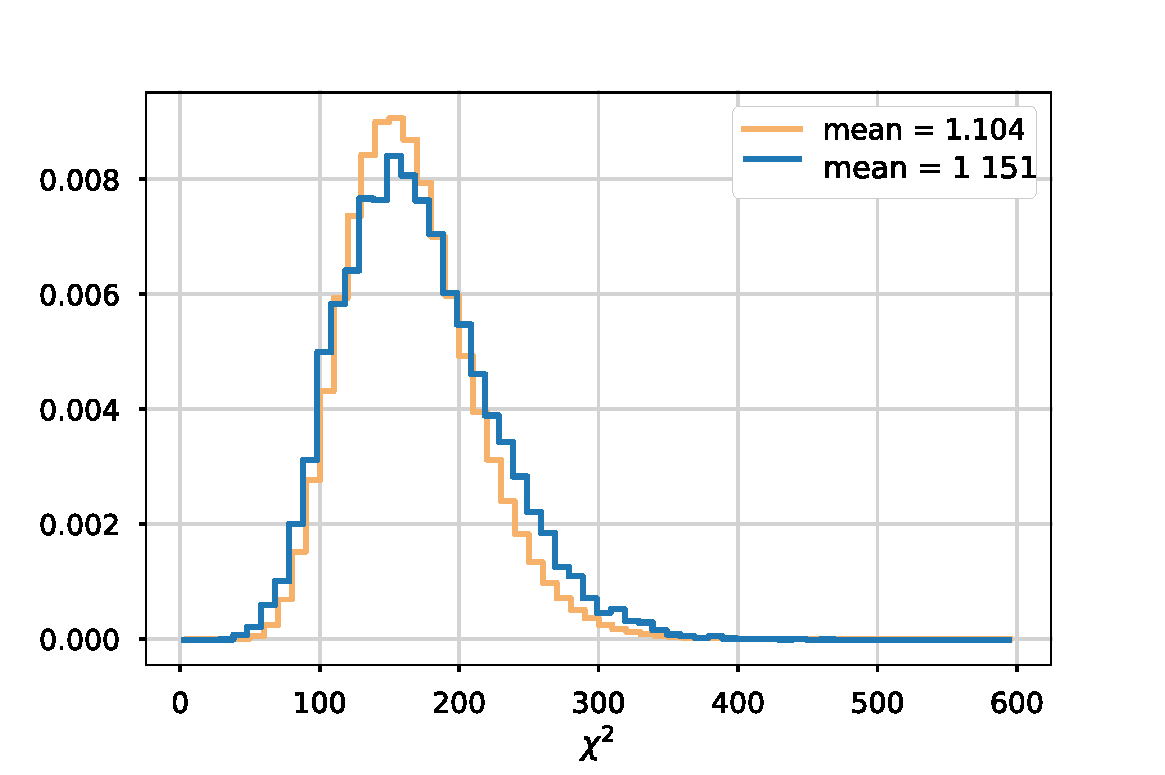
\includegraphics[width = 0.99\textwidth]{img/signals/chi2-python.pdf}
  \caption{Спектр отклонений $ \chi^2 $.}
  \label{fig:signals-chi2}
\end{figure}

По графикам видно, что:

\begin{enumerate}
    \item Распределения по форме совпадают с хи-квадрат распределением.
    \item Среднее отклонение для обоих наборов данных в пределах десятых равно единице.
\end{enumerate}
Таким образом, по результатам валидации, можно утверждать, что наша модель генератора достаточно точно описывает реальные данные и может быть использован для создания размеченных выборок кадров непрерывного сигнала для тестирования алгоритмов выделения.

\subsection{Алгоритмы выделения параметров событий из кадра}

В этой подглаве будут описаны три разработанных алгоритма выделения параметров событий. С помощью алгоритмов будут обработаны тестовые выборки, по результатам будет оценено качество работы. Тестовые выборки являются симуляцией набора с Лан10-12PCI со скоростью счета 40 кГц (которая соответствует максимальной скорости счета, ожидаемой в <<Троицк ню-масс>> ) и продолжительностью набора 35 с (тестовые выборки не идентичны друг другу, но аналогичны по параметрам).

Определим эффективную скорость счета как:
\begin{equation}
    \tau = \frac{T}{N_0} \left(1 - \frac{N}{N_0} \right),
    \label{eq:effective-dead-time}
\end{equation}
где $ T $- полное время набора, $ N $- количество распознанных событий, $ N_0 $- реальное количество событий в кадре.

В качестве метрик качества обработки будут выступать:

\begin{enumerate}
    \item скорость обработки,
    \item процент распознанных событий,
    \item процент ложноположительных срабатываний,
    \item эффективная скорость счета, определяемая по формуле \ref{eq:effective-dead-time}.
\end{enumerate}
Для определения соответствий между исходными реконструированными событиями используются следующие правила:

\begin{enumerate}
    \item Реконструированное событие соответствует исходному, если:
    \begin{enumerate}
        \item текущее реконструированное событием ближайшее к исходному по сравнению с остальными реконструированными событиями и
        \item разница между положениями пика не превышает 10 бинов (т.е. 3.2 мкс).
    \end{enumerate}
    \item Исходное событие считается наложенным, если:

    \begin{enumerate}
        \item разница между положениями пика исходного и реконструированного событий не превышает 10 бинов и
        \item соответствующее реконструированное событие имеет другое более близкое исходное событие.
    \end{enumerate}
    \item Исходное событие считается нераспознанным, если для него не существует реконструированного события с положением пика, отличным от исходного менее чем на 10 бинов.
    \item Реконструированное событие считается ложным распознаванием, если для него не существует исходного события с положением пика, отличным от реконструированного менее чем на 10 бинов.
\end{enumerate}

\begin{figure}
  \centering
  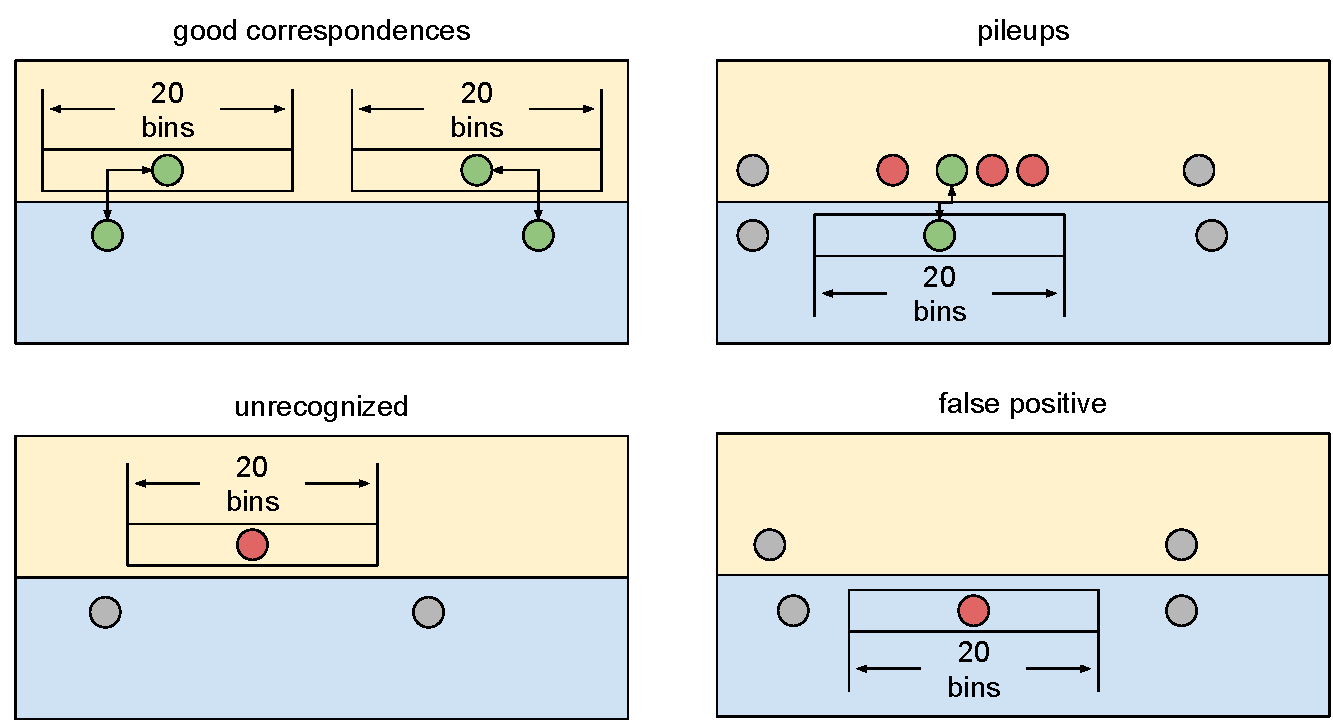
\includegraphics[width = 0.6\textwidth]{img/signals/compare-scheme.pdf}
  \caption{Правила определения соответствий между событиями. Обозначения: желтый прямоугольник содержит исходные события, голубой - восстановленные, зелеными кружками отмечены взаимно соответствующие друг другу события, красным - нераспознанные \textbackslash ложнораспознанные \textbackslash наложенные события в зависимости от примера, серыми - не относящиеся к примеру события, нарисованные для наглядности.}
  \label{fig:signals-compare-scheme}
\end{figure}

\subsection{Алгоритм 1. Simple}
Сперва был испробован тривиальный способ выделения параметров событий - поиск в кадре локальных экстремумов выше порога. Амплитуда и положение события определяется из номера бина экстремума и его значении.
Алгоритм крайне быстр в обработке и прост в реализации но страдает низкой точностью - для разделения наложений ему требуется наличие видимого изгиба между близкими событиями. Также, точность полученных амплитуды и положения могут принимать только кратные значению канала и шагу оцифровки соответственно - промежуточных значений быть не может. Стоит отметить, что из-за своей простоты алгоритм по сути не использует форму события вообще и соответственно не проводит связанных с ней коррекций, таких как коррекция на выбросы от предыдущих событий.

Результаты тестирования изображены на рисунке \ref{method-1-metrics}. На тестовом кадре не распознаны события 2 и 3. Второе событие не имеет перегиба на границе с первым, поэтому не может быть распознано как локальный экстремум и пропускается. Третье событие, хоть и имеет перегиб, попало на выброс от событий 1 и 2 и стало ниже порогового значения. Событие 4 было успешно распознано, однако из-за попадания на выбросы предыдущих событий его амплитуда исказилась. Искажение также можно увидеть на гистограмме амплитудных ошибок - асимметрия спектра справа (амплитуда исходного события больше реконструированного) вызвана отсутствием поправки на выбросы.

Несмотря на качество обработки, алгоритм все еще является быстрым и может быть полезен - на установке “Троицк ню-масс” мы используем его для визуализации набираемых данных в реальном времени как наиболее подходящий для этого.

\begin{figure}
\centering
    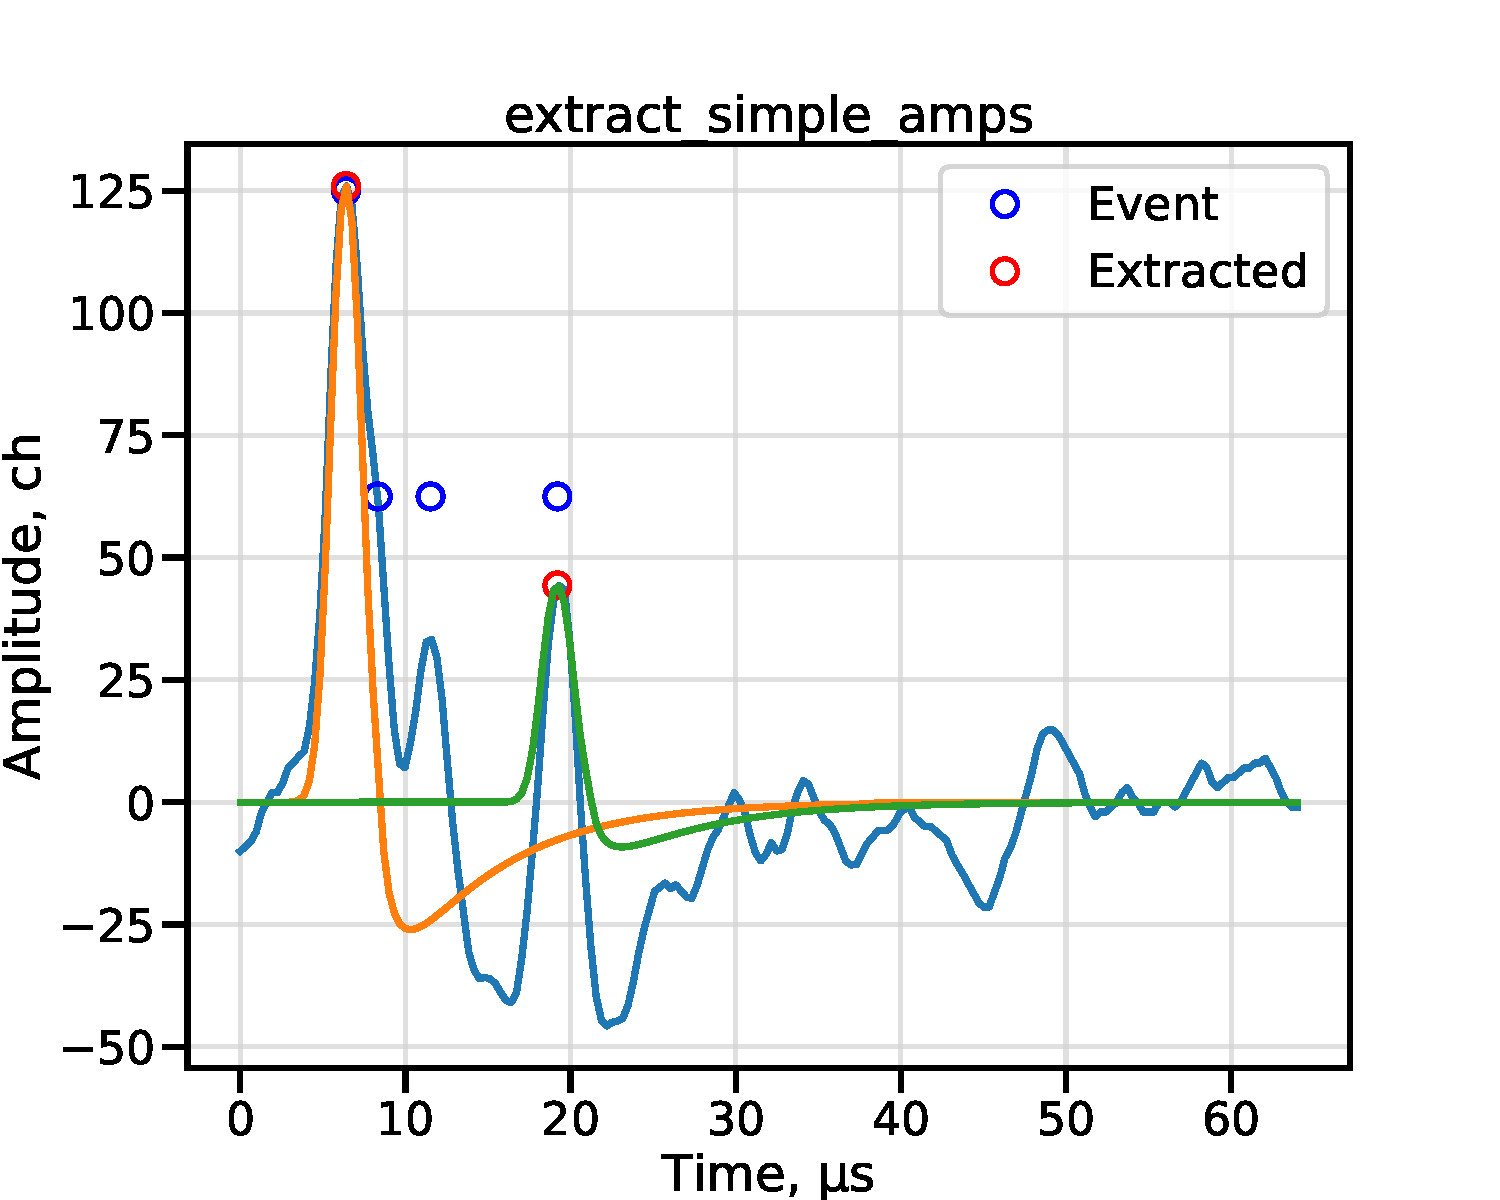
\includegraphics[width=0.40\linewidth]{img/signals/method_1/frame.pdf} 	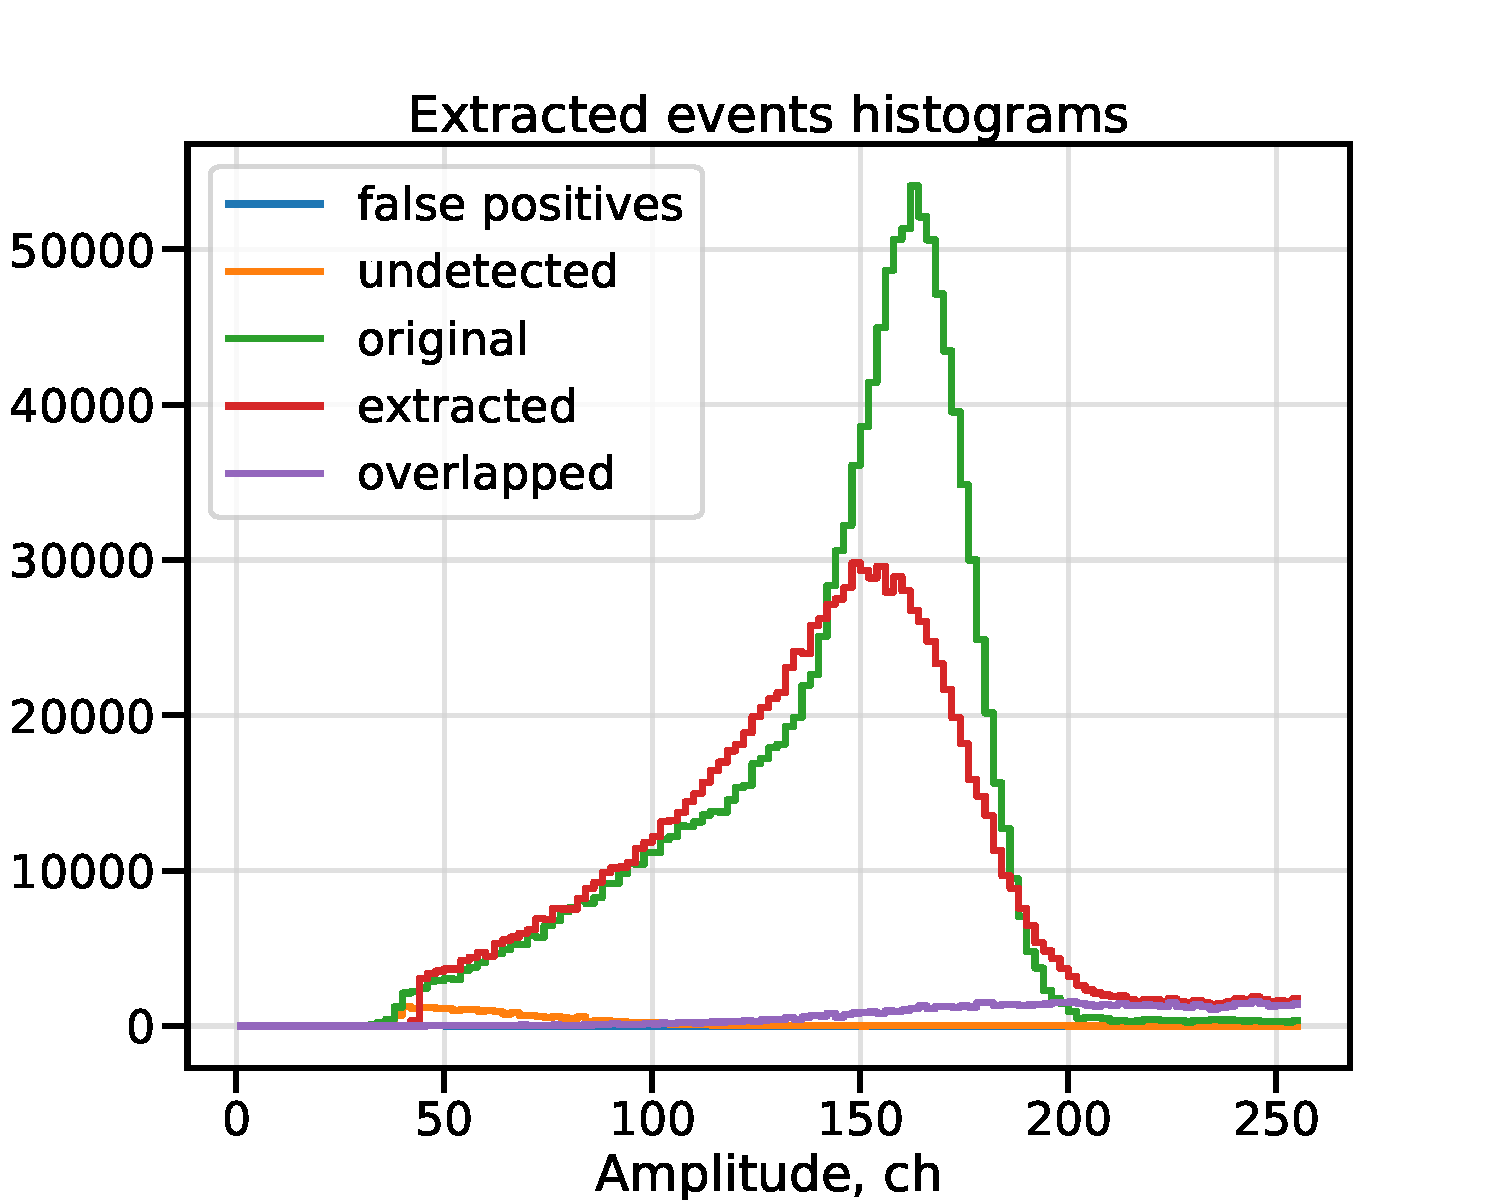
\includegraphics[width=0.40\linewidth]{img/signals/method_1/hist.pdf} \\
    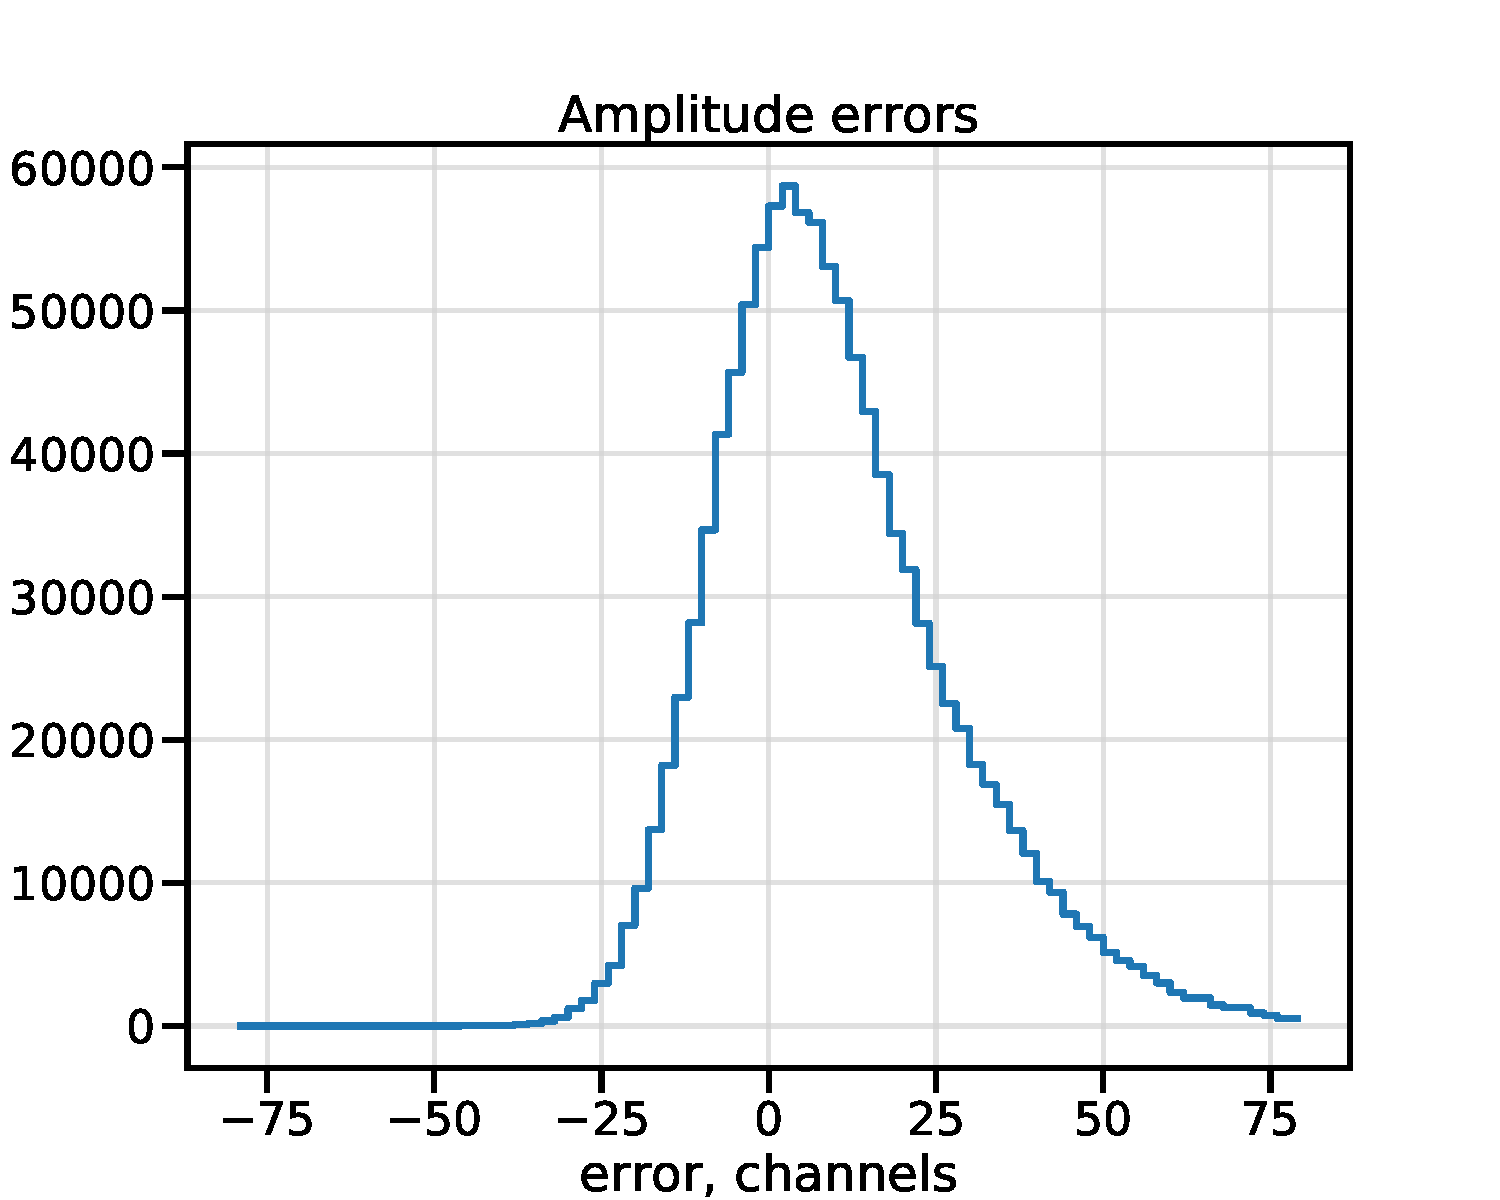
\includegraphics[width=0.40\linewidth]{img/signals/method_1/ampl.pdf} 	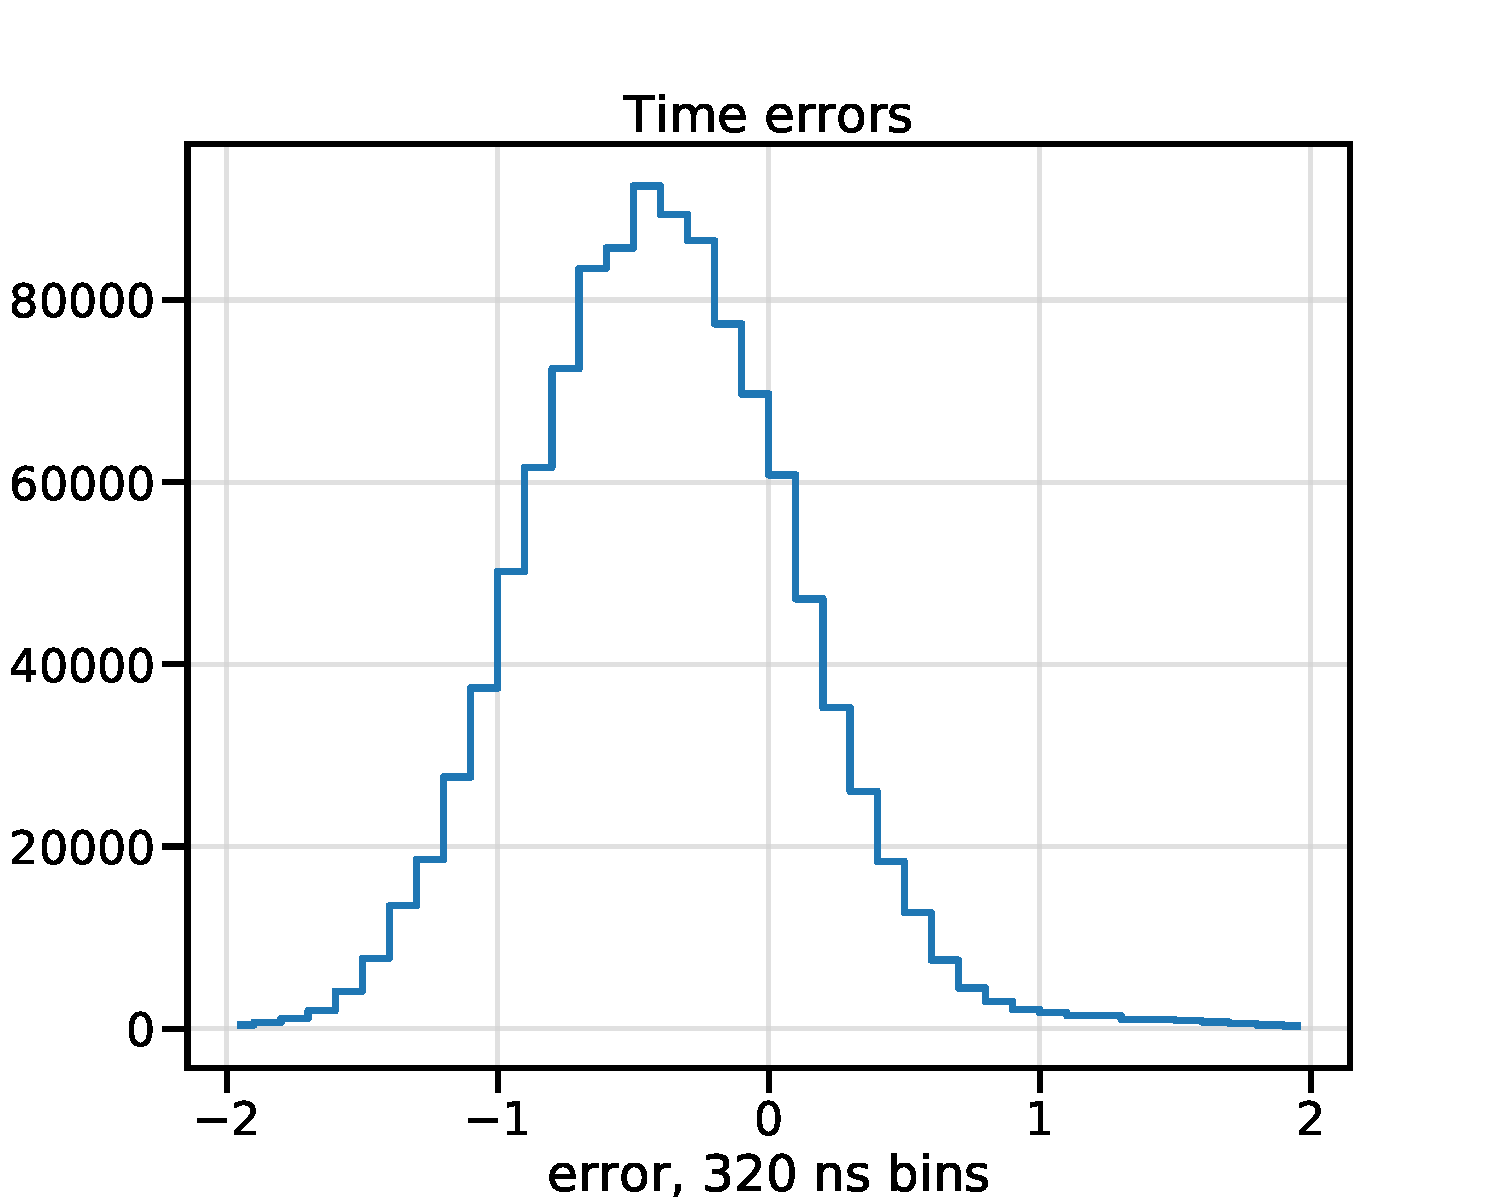
\includegraphics[width=0.40\linewidth]{img/signals/method_1/time.pdf} \\
    \caption{Результаты тестирования алгоритма 1. На верхнем левом графике приведен пример обработки на конкретном примере. Справа сверху представлены распределения всех типов событий. Внизу слева и справа показаны гистограммы ошибок по амплитудам и положениям соответственно.}
    \label{method-1-metrics}
\end{figure}

\subsection{Алгоритм 2. Approximate After-pulses}
Алгоритм является улучшенным вариантом Simple с добавлением коррекции на выбросы. Добавлены новые правила:
\begin{enumerate}
    \item После определения положений событий через локальные экстремумы, считывание амплитуд осуществляется последовательно от события к событию строго слева направо.
    \item После считывания амплитуды в бине события, из кадра удаляется форма, соответствующая событию с параметрами текущего извлеченного события. Т.о. из данных удаляется само событие и его влияние на другие события. Т.к. обход идет слева направо, амплитуда обрабатываемого события будет скорректированной, т.к. все более ранние события уже обработаны и удалены из кадра.
\end{enumerate}

Результаты тестирования показаны на рисунке \ref{method-2-metrics}.Как и в Simple, положения событий определяются только один раз вначале. Такой выбор был сделан ради скорости и стабильности обработки. Из-за этого, по той же причине что и в Simple события 2 и 3 остались не распознанными. Однако теперь амплитуда четвертого события скорректировалась (неполностью, т.к. события 2 и 3 не были удалены из кадра). Коррекцию на выбросы можно также наблюдать на распределении ошибок восстановления амплитуд - форма стала заметно симметричнее.
Потенциально, алгоритм можно ускорить и добиться производительности на уровне Simple. Для этого вместо вычитания всей формы события из кадра нужно вычитать ее только из бинов с пиками событий.

\begin{figure}
\centering
    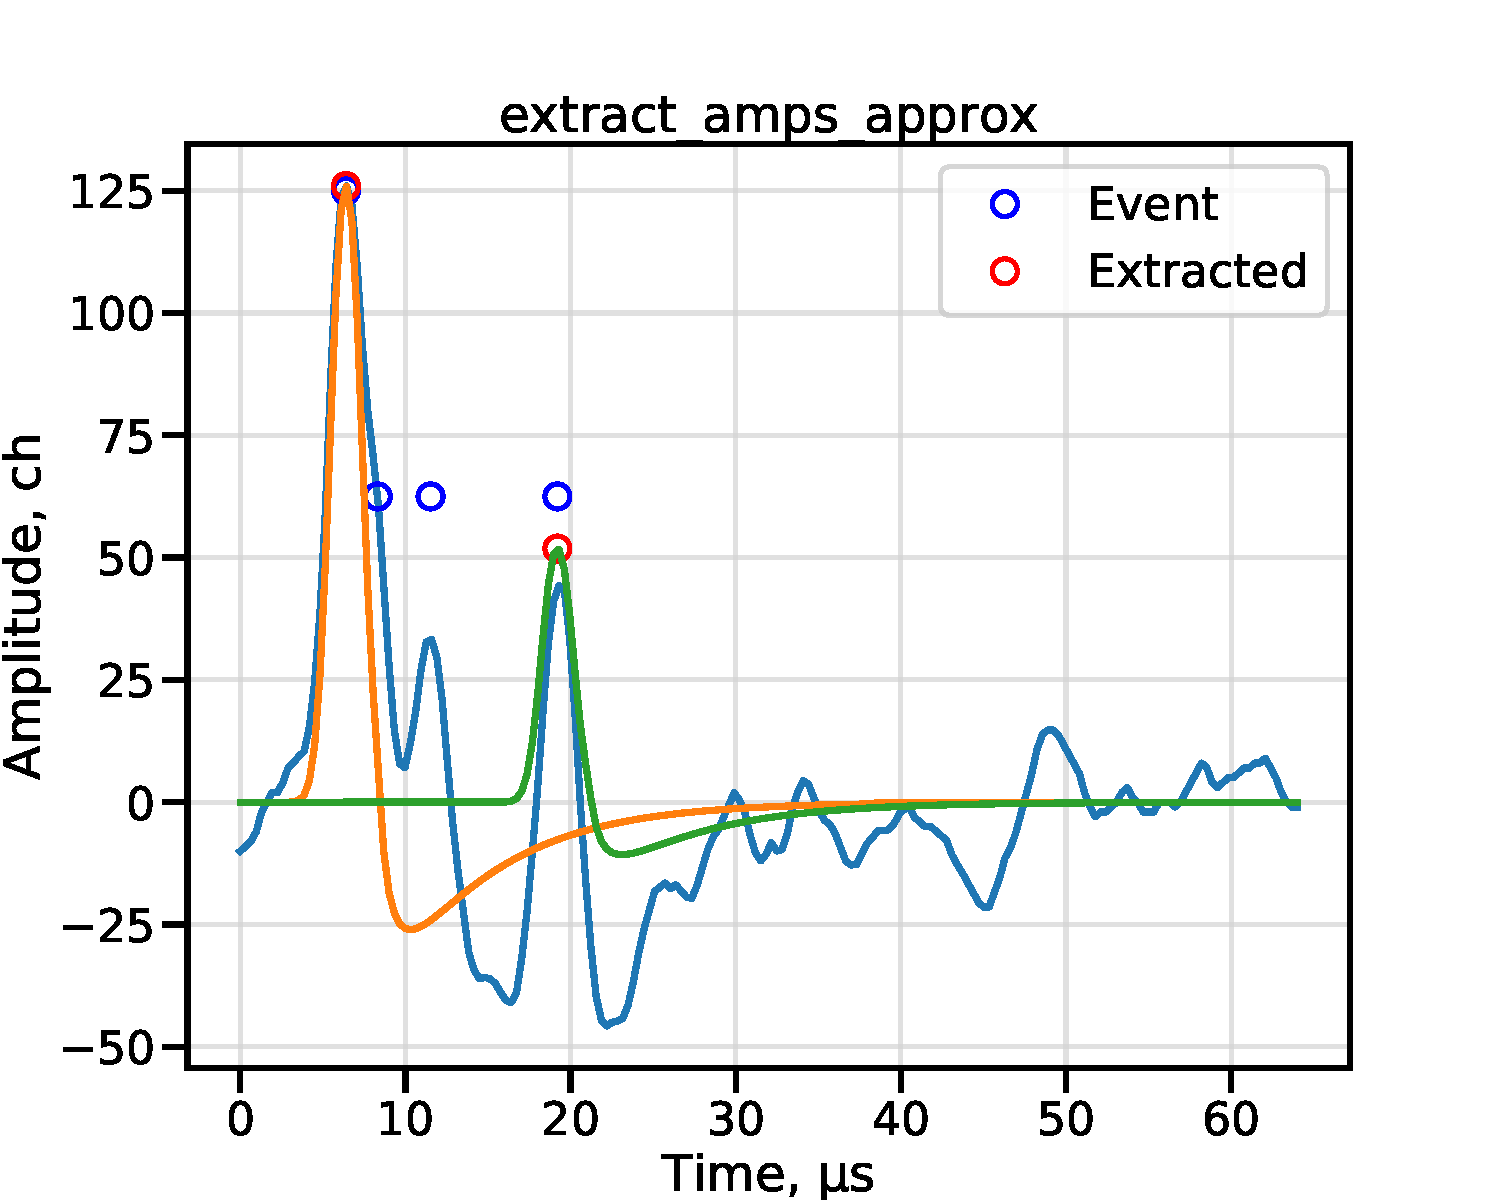
\includegraphics[width=0.40\linewidth]{img/signals/method_2/frame.pdf} 	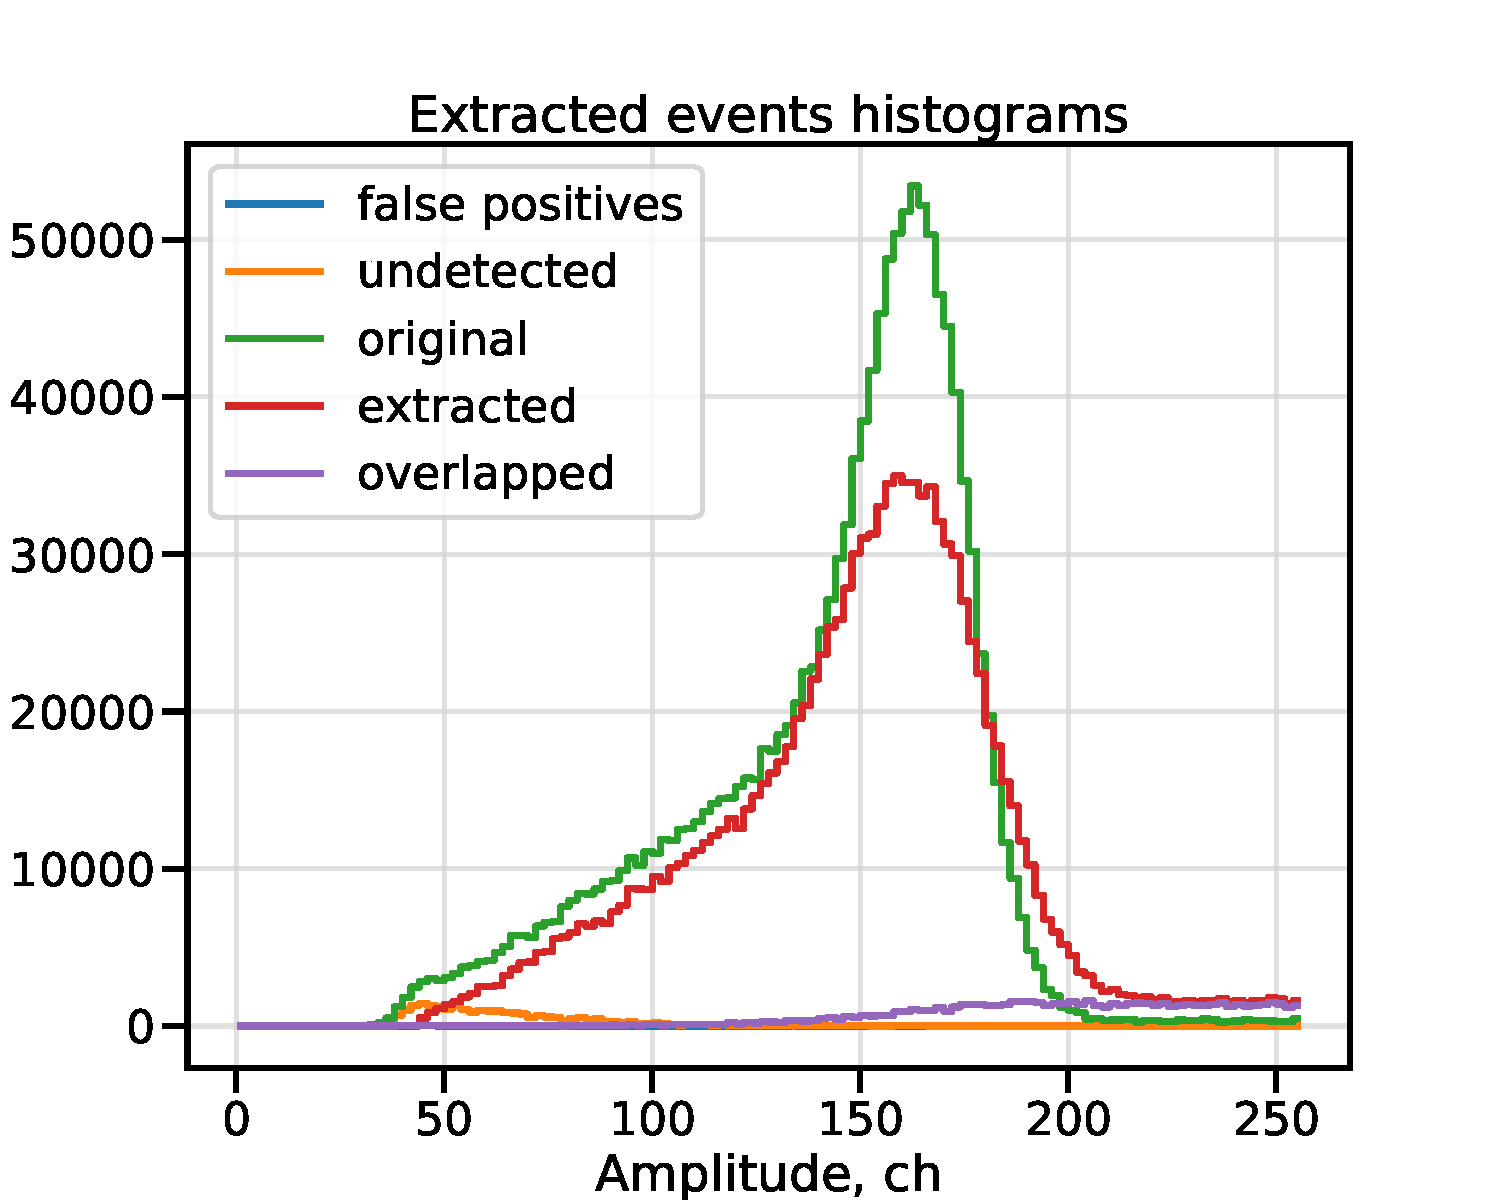
\includegraphics[width=0.40\linewidth]{img/signals/method_2/hist.pdf} \\
    \includegraphics[width=0.40\linewidth]{img/signals/method_2/ampl.pdf} 	\includegraphics[width=0.40\linewidth]{img/signals/method_2/time.pdf} \\
    \caption{Результаты тестирования алгоритма 2}
    \label{method-2-metrics}
\end{figure}

\subsection{Алгоритм 3. Front fit}
Данный алгоритм разрабатывался с целью уменьшить количество нераспознанных событий с помощью обнаружения новых событий после коррекции на выбросы.

Изменен способ поиска - теперь за итерацию ищется только одно событие (самое раннее). Условие поиска - первое превышение порога в кадре. После нахождения алгоритм производит фитирование формы события по нескольким точкам фронта (окрестность порогового бина) и восстанавливает параметры. Выбор окрестности фитирования обусловлен временной очередностью: самый ранний фронт в кадре чаще всего является фронтом первого события и поэтому не искажается. После извлечения параметров, реконструированная форма удаляется из кадра и процесс повторяется.

Такой подход позволяет:

\begin{itemize}
    \item Определять наложенные события не имеющие разделения в виде перегиба.
    \item Определять события, изначально имеющие амплитуду ниже порога.
    \item За счет фитирования точность извлекаемых параметров меньше размера бина по положению и меньше канал по амплитуде.
\end{itemize}

\begin{figure}
\centering
    \includegraphics[width=0.40\linewidth]{img/signals/method_3/frame.pdf} 	\includegraphics[width=0.40\linewidth]{img/signals/method_3/hist.pdf} \\
    \includegraphics[width=0.40\linewidth]{img/signals/method_3/ampl.pdf} 	\includegraphics[width=0.40\linewidth]{img/signals/method_3/time.pdf} \\
    \caption{Результаты тестирования алгоритма 3}
    \label{method-3-metrics}
\end{figure}

Результаты тестирования показаны на рисунке \ref{method-3-metrics}. Все события в тестовом кадре успешно распознаны. Спектры амплитудных и временных ошибок симметричны. По восстановленной амплитудной гистограмме видно, что алгоритм распознал намного больше событий по сравнению с алгоритмами 1 и 2. Однако вместе с этим увеличилось количество ложноположительных срабатываний (стало около 2\% против 0.01\% у алгоритмов 1 и 2). Такой большой процент вносит значительное и неизвестное искажение при обработке и делает бессмысленным дальнейший анализ данных.

Нозиком А.А. был предложен вариант постобработки позволяющий эффективно фильтровать ложные события. Способ заключается в:

\begin{enumerate}
    \item введению искусственного мертвого времени;
    \item вырезание групп восстановленных событий, в которых каждое событие имеет соседнее событие на расстояние меньше чем искусственное мертвое время, вместе с занимаемыми бинами;
    \item корректировка времени набора на вырезанные области.
\end{enumerate}
За счет особенностей распределения Пуассона, фильтр удаляет из выборки в основном аномальные группы близких событий, не подчиняющиеся ему. Также удаляется часть настоящих событий, однако зная время обрезки и их подчинение процессу Пуассона, можно скорректировать создаваемое искажение. Более подробно метод описан в \cite{1810.07024}.

На рисунке \ref{fig:method-3-crop} изображен график зависимости количества событий по типам от вводимого мертвого времени. При мертвом времени равным 6 бинам (1.92 мкс) постобработка удаляет практически все двойные наложения (до 0.01\%) и 15\% всех событий.

\begin{figure}
  \centering
  \includegraphics[width = 0.9\textwidth]{img/signals/method_3/crop.png}
  \caption{Соотношение типов событий в зависимости от размера обрезки.}
  \label{fig:method-3-crop}
\end{figure}

\subsection{Сравнение}

В таблице \ref{tbl:methods-compare-1} приведены результаты тестирования всех трех алгоритмов (время сбора данных составляет 35 с и скорость счета составляет 40 кГц). Эффективное мертвое время определяется формулой \ref{eq:effective-dead-time}.

\begin{table}
\centering
    \begin{tabular}{|l|l|l|l|}
        \hline
         & Simple & Approx spikes & Front fit (with filter) \\
        \hline
        Время работы, \% & 61.1 & 158.8 & 9771.5 \\
        \hline
        Распознаваний, \% & 88.34 & 88.29 & 97.999 \\
        \hline
        Нераспознанных,  \% & 11.66 & 11.71 & 02.01 \\
        \hline
        Ложноположительные,\% & 0.01 & 0.01 & 0.01 \\
        \hline
        Мертвое время, мкс & 3.195 & 3.167 & 1.92 \\ 
        \hline
    \end{tabular} 
    \caption{Сравнение алгоритмов}
    \label{tbl:methods-compare-1}
\end{table}

Первый и второй алгоритмы дают одинаковые количественные результаты и имеют одинаковое эффективное мертвое время около 3 мкс. Однако второй метод корректирует амплитуды на выбросы от предыдущих событий. Потенциально из-за коррекции алгоритм 2 может извлечь больше событий, но это негативно скажется на его стабильности и производительности. Алгоритм 3 с фильтрацией по искусственному мертвому времени имеет мертвое время 2 мкс (равно введенному искусственному), выделяет практически на 10\% больше событий и имеет точность выше единиц АЦП. Помимо достоинств, алгоритм “Front fit” имеет некоторые недостатки, такие как:

\begin{itemize}
    \item Использование фильтрации уменьшает выборку на 15\% и соответственно уменьшает статистическую точность результатов. 
    \item Алгоритм работает очень медленно, т.к. написан на Python и в обработке производит фитирование кривой.
\end{itemize}

\section{Обобщение алгоритмов и оптимизация системы обработки}

Продолжительная эксплуатация реализованных алгоритмов выделения параметров событий показала следующие недостатки:

\begin{enumerate}
    \item Скорость. За несколько сеансов с Лан10-12PCI объем набранных данных достиг 500 Гб и вопрос производительности встал на первое место.
    \item Появилось требование к точности времени реконструированного события. Точное время необходимо для проведения соответствующего временного анализа и процедур контроля качества, описанных ~в {\textbackslash} cite \{Nozik: 2018zko\}. Алгоритмы 1, 2 используют простые методы поиска пиков, которые дают время только с точностью в один бин, чего недостаточно. Алгоритм 3 обладает достаточной точностью, однако скорость работы не позволяет серьезно использовать его.
    \item Ограниченность инструментария. Невозможность использования функций при обработке. Необходимость реализации алгоритмов в виде тензорных преобразований.
    \item Обобщение алгоритмов. При анализе данных было обнаружено, что форма события меняется, притом новая форма не имеет аналитической формулы. Также оказалось, что свойства шума тоже меняются.
\end{enumerate}

Для увеличения производительности, было решено сменить язык программирования с Python на Kotlin(\cite{jemerov2016kotlin}), который статически компилируется, имеет преимущество совместимости с библиотеками Java, имеет современный и удобный синтаксис и возможность использовать библиотеки на нескольких платформах компиляции в будущем. Это позволило увеличить скорость анализа до десяти раз по сравнению с версией Python с той же функциональностью и использовать недоступные на Python возможности.

\subsection{Обобщенный генератор шума}

Для сеанса 2017\_11 был построен амплитуд спектр шума. В нем обнаружились расхождения со спектром, используемом в. В связи с этим был также перестроен спектр для 2017\_05. Как оказалось, он также не совпадает со спектром из статьи и больше похож на шум сеанса 2017\_11. Скорее всего это связано с увеличением скорости счета и появлением базовой линии в сигнале.

Использование старой реализации шумогенератора на датасете 2017\_11 ~потребовало бы повторной ручной подстройки количества этапов и степеней сглаживания под новые данные. С учетом перевода кода на Kotlin такую подстройку стало затруднительно проводить. Поэтому мы решили изменить способ генерации шума, обобщив его на произвольный вид шума.

Работа обобщенного генератора шума разделена на 2 части:

\begin{enumerate}
    \item Создание индексированной выборки фрагментов шумов
    \item Генерация шума по созданной выборке
\end{enumerate}

Для создания выборки фрагментов шумов используются также начала в набранных кадрах (в нашем генераторе мы берем первые 35 бинов). Элемент выборки - фрагмент из начала кадра максимальной длины (и не меньше заданной - 10 бинов), пересекающий нуль с обоих концов. В качестве индекса берется пара из значений первых двух бинов. Выборка записывается на диск в виде двух файлов - бинарный файл с последовательно записанными фрагментами и файл с сериализованной хеш картой, содержащей списки отступов фрагментов в файле для каждого индекса (алгоритм был реализован в нескольких вариантах, в т.ч. с использованием СУБД в качестве хранилища фрагментов, однако вариант с двумя файлами оказался самым быстрым).

Генерация шума происходит следующим образом:

\begin{enumerate}
    \item Из бинарного файла считывается произвольный фрагмент
    \item При запросе из начала текущего фрагмента извлекается отдается один бин. Операция повторяется пока длина текущего запроса больше 2 бинов.
    \item Оставшиеся 2 бина текущего фрагмента преобразовываются в индекс, по которому из хеш карты берется список отступов фрагментов имеющих этот индекс.
    \item Из списка случайным образом выбирается отступ, по нему из файла считывается фрагмент
    \item Считанный фрагмент становится текущим. Переход к п.2. 
\end{enumerate}

На рисунке \ref{fig:signals-noise-generator-workflow} показан принцип работы генератора.

\begin{figure}
  \centering
  \includegraphics[width = 0.6\textwidth]{img/signals/noise-generator-workflow.pdf}
  \caption{Принцип работы обобщенного генератора шума.}
  \label{fig:signals-noise-generator-workflow}
\end{figure}

Таким образом мы генерируем шум, склеенный из реальных фрагментов. Совпадение 2 бинов на границе примыкающих фрагментов обеспечивает гладкость перехода. Т.к. для генерации используются только реальные данные - статистически, генерируемый шум будет неотличим от настоящего, что подтверждается сравнением, показанном на рисунке \ref{fig:signals-noise-generator-dist-new}. Это также означает, что алгоритму не требуется дополнительных ручных настроек под конкретный тип шума.

\begin{figure}
  \centering
  \includegraphics[width = 0.8\textwidth]{img/signals/noise_dist_new.png}
  \caption{Сравнение шумовых спектров.}
  \label{fig:signals-noise-generator-dist-new}
\end{figure}

\subsection{Обобщенный генератор формы события}

Анализ данных показал, что формы событий в датасете 2017\_11 также отличаются от сеанса 2017\_05 (см рисунок \ref{fig:signals-event-shapes-2017-11}). Более того, теперь в выбросе после события появились осцилляции и подобрать аналитическую функцию для описания формы уже не получится. Всвязи с этим мы решили обобщить алгоритм генерации события и убрать из него ручную настройку.

\begin{figure}
  \centering
  \includegraphics[width = 0.8\textwidth]{img/signals/event_shapes_2017_11.png}
  \caption{Усредненные формы событий.}
  \label{fig:signals-event-shapes-2017-11}
\end{figure}

Также как и в старом генераторе, описанном в , сначала строятся усредненные формы событий по группам амплитуд. Затем, по формам строятся интерполяционные сплайны, по которым находятся точные положения пиков. Отцентрированные по пику сплайны форм переносятся на новые временные сетки, имеющие одинаковые координаты узлов. Из набора сеток для амплитудных групп строится двумерная сетка,
амплитудными координатами узлов является амплитуда пика усредненной формы в группе, временными координатами - координаты узлов формы (они одинаковые для всех групп). На полученной сетке строится бикубический сплайн.

Если параметры точки генерируемого события находятся внутри области интерполяции (в нашем генераторе область интерполяции слегка усекается по амплитудному диапазону, т.к. на границах интерполятор выдает артефакты) - значение определяется интерполяцией. 
Если амплитуда генерируемой точки выходит за пределы области интерполяции - значение определяется линейной экстраполяцией граничного значения.
Если положение генерируемой точки выходит за пределы области интерполяции - значение приравнивается нулю вне зависимости от ее амплитуды.

\subsection{Валидация генератора}
Аналогично подглаве \ref{generator-validation-1} были построены $ \chi^2 $ отклонения для реального и смоделированного сигналов. Параметры событий извлекались параболической интерполяцией по 5 точкам в окрестности локального максимума выше порога. Результат показан на рисунке \ref{fig:signals-chi2-kotlin}. Среднее значение для обоих распределений одинаково, $ \chi^2 $ для реального датасета выглядит более размытым. По проведенному сравнению $ \chi^2 $ распределений можно сказать, что алгоритм моделирования создает совпадающий с реальным сигнал.

\begin{figure}
  \centering
  \includegraphics[width = 0.8\textwidth]{img/signals/chi2-kotlin.png}
  \caption{Спектр отклонений $ \chi^2 $.}
  \label{fig:signals-chi2-kotlin}
\end{figure}

\subsection{Алгоритм 4. Fast fit}
Этот алгоритм написан на Kotlin. В основе лежит Алгоритм 3. Некоторые этапы изменены в целях ускорения работы. Схему работы можно описать следующей последовательностью:

\begin{enumerate}
    \item Поиск самого левого локального максимума выше порога (максимум определяется как самый большой бин в плавающем окне размером 5 бинов)
    \item Извлечение параметров события с помощью параболического фитирования по 5 точкам в окрестности локального максимума.
    \item Сохранение полученных параметров.
    \item Вычитание из кадра реконструированной по параметрам формы события.
    \item Переход к п.1.
\end{enumerate}

По сравнению с Алгоритмом 3, здесь изменен способ определения параметров события - ~используется параболическое фитирование в окрестности пика. Плюсы такого подхода - это больше ускорение за счет упрощенного фитирования и более устойчивая область фитирования (т.к. отношение signal\textbackslash noise выше, чем на фронте события). Недостатком является более высокий шанс пропустить самое раннее событие и попасть на следующее, имеющее искажение.

\begin{figure}
\centering
	\includegraphics[width=0.80\linewidth]{img/signals/method_4/hists.png} \\
    \includegraphics[width=0.80\linewidth]{img/signals/method_4/crop.png}
    \caption{Результаты тестирования алгоритма 4}
    \label{method-4-metrics}
\end{figure}

\begin{table}
\centering
    \begin{tabular}{|p{0.10\textwidth}|p{0.16\textwidth}|p{0.16\textwidth}|p{0.16\textwidth}|p{0.16\textwidth}|p{0.16\textwidth}|}
        \hline
         & Время работы, \% & распозн., \% & нераспозн., \% & ложнопол. ,\% & мертвое время, мкс \\
        \hline
        Fast fit & 405.7 & 96.57 & 3.45 & 0.03 & 2.24 \\ 
        \hline
    \end{tabular} 
    \caption{Метрики алгоритма 4}
    \label{tbl:methods-compare-2}
\end{table}

Результаты тестирования представлены на рисунке \ref{method-4-metrics} и в таблице \ref{tbl:methods-compare-2}. По результатам тестирования алгоритмы 3 и 4 похожи. Fast fit генерирует похожее число двойных наложений. Их также можно убрать с помощью фильтрации в обмен на 15\% выборки. Преимуществом алгоритма является скорость - превышающая алгоритм 3 в 24 раза.

Для подробного анализа в проект были добавлены программы, которые выводят графики обработки кадра в случаях, если в нем произошло наложение, появилось ложноположительное срабатывание или потеряно событие.

Просмотрев несколько кадров , мы заметили что наложения практически всегда имеют одну и ту же природу: расстояние и отношения амплитуд между исходными сигналами появляются в такой комбинации, что суммарная форма по ширине близка к ширине одиночного события с пиком амплитуды примерно равным сумме исходных амплитуд.

В случае, когда исходные события находятся чуть дальше друг от друга и суммарная форма превышает ширину одиночного события, алгоритм может генерировать ложноположительное срабатывание. Просмотр таких случаев показал, что это происходит по двум сценариям:

\begin{enumerate}
    \item Два события расположены относительно симметрично и пик их суммарной формы находится посередине исходных пиков. В этом случае алгоритм привяжется к пику ~конечной формы (из-за параболического фитирования в области максимума) и выделит несуществующее событие. Реальные исходные события как правило тоже выделяются, но с меньшими амплитудами, т.к. часть их ушла на ложноположительное. Пример такого случая изображен в таблице ниже справа.
    \item Два близких события образуют несимметричную конченную форму. В этом случае, как правило, выделяются оба исходных события выделяются достаточно хорошо, однако из-за ошибок определения пиков (связанных со способом поиска) после выделения исходных событий в форме остается “излишек”, который интерпретируется как событие. Обычно ложноположительное срабатывание такого типа имеет небольшую амплитуду и может быть эффективно отфильтровано.
\end{enumerate}

Оба сценария проиллюстрированы на рисунке \ref{method-4-artifacts}.
\begin{figure}
\centering
	\includegraphics[width=0.40\linewidth]{img/signals/artifacts/overlap.png}
    \includegraphics[width=0.40\linewidth]{img/signals/artifacts/false_positive.png}
    \caption{Типичные случаи наложения (слева) и ложного срабатывания (справа). }
    \label{method-4-artifacts}
\end{figure}

\subsection{Алгоритм 5. Double Fit}
Во время просмотра случаев выделения параметров событий, при которых возникали ложноположительные срабатывания была выявлена закономерность - в большинстве таких ситуаций происходит также нарушение очередности обработки наложенных событий, т.е. следующее выделенное событие будет иметь более раннее время возникновения чем текущее. Т.о. нарушение очередности можно использовать как сигнал наличия наложения.

Алгоритм Double Fit представляет собой алгоритм Fast fit с дополнительной обработкой в случае нарушения очередности.

Схема работы:

\begin{enumerate}
    \item Запись текущего состояния в стек.
    \item Выделение события аналогично алгоритму Fast fit.
    \item Проверка очередности последних двух событий.
    \begin{enumerate}
        \item Переход к п.1, если очередность соблюдена или расстояние между событиями больше 8 бинов.
        \item в противном случае:
        \begin{enumerate}
            \item Откат состояния до этапа, на котором выделенное событие было левее текущего. Одновременно ищутся самое левое и самое правое события отмененные откатом.
            \item Выделение двойного наложения фитированием. Функция - сумма двух форм событий, область интерполяции - промежуток между крайними отмененными событиями.
            \item Запись извлеченной пары событий.
            \item Вычитание извлеченных событий из кадра.
            \item Переход к п.1.
        \end{enumerate}
    \end{enumerate}
\end{enumerate}

Работа алгоритма опирается на стек состояний, хранящий историю предыдущих этапов и возможность отката на предыдущие состояния. При откате назад выделенные на текущем этапе события удаляются из массива результатов, а кадр обращает вычитание формы из себя.

Т.е. при нарушении очередности алгоритм возвращает состояния до последнего правильного и меняет способ выделения на фитирование одновременно двух событий по полной форме.

В результате качество выделения значительно улучшается - алгоритм генерирует 0.03\% ложноположительных срабатываний и не требует дополнительных постобработок. Результаты тестирования приведены на рисунке \ref{method-5-metrics} и в таблице \ref{tbl:methods-compare-3}.

\begin{figure}
\centering
	\includegraphics[width=0.40\linewidth]{img/signals/method_5/amps.png} 
    \includegraphics[width=0.40\linewidth]{img/signals/method_5/time.png} \\
    \includegraphics[width=0.80\linewidth]{img/signals/method_5/hists.png}
    \caption{Результаты тестирования алгоритма 5}
    \label{method-5-metrics}
\end{figure}

\begin{table}
\centering
    \begin{tabular}{|p{0.10\textwidth}|p{0.16\textwidth}|p{0.16\textwidth}|p{0.16\textwidth}|p{0.16\textwidth}|p{0.16\textwidth}|}
        \hline
         & Время работы, \% & распозн., \% & нераспозн., \% & ложнопол. ,\% & мертвое время, мкс \\
        \hline
        Double fit & 591.4 & 96.3 & 3.7 & 0.03 & 0.96 \\ 
        \hline
    \end{tabular}
    \caption{Метрики алгоритма 5}
    \label{tbl:methods-compare-3}
\end{table}

\todo[inline]{Здесь или в начале главы обязательно должен быть кусок с объяснением того, почему обработка событий так важна. Надо объяснить, что мертвое время является одним из главных источников систематической погрешности (есть статье с пропозалом по стерильным нейтрино. Также надо привести цифры по потере статистики из-за мертвого времени при разных загрузках. Прямо график сделать)}

\chapter*{Заключение}
\addcontentsline{toc}{chapter}{Заключение}

\todo[inline]{Тут должны быть положения, выносимые на защиту, так что надо пунктиков побольше и поподробнее, также надо явно указать, какой вклад эта работа внесла в эксперимент (не стесняясь особо) и в каких статьях опубликованы результаты}.

В данной работе было выполнены следующие этапы:
\begin{enumerate}
    \item Модернизирована архитектура системы сбора данных установки <<Троицк ню-масс>>. Исходная система, выполненная в виде монолитной программы, заменена на набор отдельных модулей (микросервисов). Каждый модуль может работать самостоятельно, имеет свой логически полный набор операций и инкапсулирует в себе внутреннюю логику обработки и взаимодействие с аппаратной частью системы. Между собой модули взаимодействуют через ethernet соединение по протоколу TCP/IP в формате Datafore Envelope, который также был разработан и реализован в ходе работы.
    \item Успешно реализованы два расширения для модернизированной системы сбора данных:
    \begin{itemize}
        \item В рамках коллаборации с TRISTAN на установке <<Троицк ню-масс>> было проведено тестирование прототипа детектора для эксперимента <<Katrin>>. Для системы сбора данных был написан модуль, реализующий логику набора событий через АЦП Dante, управляющее прототипом детектора.
        \item При переходе на поиски стерильных нейтрино в система сбора данных была добавлена более быстрая АЦП Лан10-12PCI - для этого был написан новый модуль, реализующий процесс набора непрерывного сигнала с помощью платы и подключающийся в систему последовательно со старой системой записи событий.
    \end{itemize}
    \item Разработаны алгоритмы выделения параметров событий (амплитуды и положения) из непрерывного сигнала, снятого платой Лан10-12PCI. При разработке также был созданы: генератор, симулирующих сигнал АЦП с событиями, и тестовый фреймворк для оценки качества работы разрабатываемых алгоритмов. Для данных <<Троицк ню-масс>> при выделении параметров событий удалось добиться эффективного мертвого времени порядка 0.9 мкс для средней длины события 3-5 мкс и размера бина в 320 нс. Разработанные алгоритмы были обобщены на произвольную форму события и шумов, код реализаций с инструкциями воспроизведению изложенных в работе результатов был выложен в открытый доступ в репозитории \cite{signal-utils}\cite{lan10-processing}.
\end{enumerate}

\printbibliography
\end{document}
